\documentclass[11pt,a4paper,oneside]{report}             % Single-side
%\documentclass[11pt,a4paper,twoside,openright]{report}  % Duplex

%\PassOptionsToPackage{chapternumber=Huordinal}{magyar.ldf}
\usepackage{t1enc}
\usepackage[latin2]{inputenc}
\usepackage{amsmath}
\usepackage{amssymb}
\usepackage{enumerate}
\usepackage[thmmarks]{ntheorem}
\usepackage{graphics}
\usepackage{epsfig}
\usepackage{listings}
\usepackage{color}
%\usepackage{fancyhdr}
\usepackage{lastpage}
\usepackage{anysize}
\usepackage[magyar]{babel}
\usepackage{sectsty}
\usepackage{setspace}  % Ettol a tablazatok, abrak, labjegyzetek maradnak 1-es sorkozzel!
\usepackage[hang]{caption}
\usepackage{hyperref}

%\usepackage{graphicx}
%\usepackage{wrapfig}
%\usepackage{lscape}
%\usepackage{rotating}
%\usepackage{epstopdf}

\usepackage{array}
\usepackage{multirow}
%--------------------------------------------------------------------------------------
% Main variables
%--------------------------------------------------------------------------------------
\newcommand{\vikszerzo}{V�ri J�nos}
\newcommand{\vikkonzulens}{Dr. Dud�s �kos}
\newcommand{\vikcim}{N-test szimul�ci� p�rhuzamos k�rnyezetben}
\newcommand{\viktanszek}{Automatiz�l�si �s Alkalmazott Informatikai Tansz�k}
\newcommand{\vikdoktipus}{Diplomaterv}
\newcommand{\vikdepartmentr}{V�ri J�nos}

%--------------------------------------------------------------------------------------
% Page layout setup
%--------------------------------------------------------------------------------------
% we need to redefine the pagestyle plain
% another possibility is to use the body of this command without \fancypagestyle
% and use \pagestyle{fancy} but in that case the special pages
% (like the ToC, the References, and the Chapter pages)remain in plane style

\pagestyle{plain}
%\setlength{\parindent}{0pt} % ?ttekinthet?bb, angol nyelv? dokumentumokban jellemz?
%\setlength{\parskip}{8pt plus 3pt minus 3pt} % ?ttekinthet?bb, angol nyelv? dokumentumokban jellemz?
\setlength{\parindent}{12pt} % magyar nyelv? dokumentumokban jellemz?
\setlength{\parskip}{0pt}    % magyar nyelv? dokumentumokban jellemz?

\marginsize{35mm}{25mm}{15mm}{15mm} % anysize package
\setcounter{secnumdepth}{0}
\sectionfont{\large\upshape\bfseries}
\setcounter{secnumdepth}{2}
\singlespacing
\frenchspacing
%--------------------------------------------------------------------------------------
%	Setup hyperref package
%--------------------------------------------------------------------------------------
\hypersetup{
    bookmarks=true,            % show bookmarks bar?
    unicode=false,             % non-Latin characters in Acrobat?s bookmarks
    pdftitle={\vikcim},        % title
    pdfauthor={\vikszerzo},    % author
    pdfsubject={\vikdoktipus}, % subject of the document
    pdfcreator={\vikszerzo},   % creator of the document
    pdfproducer={Producer},    % producer of the document
    pdfkeywords={keywords},    % list of keywords
    pdfnewwindow=true,         % links in new window
    colorlinks=true,           % false: boxed links; true: colored links
    linkcolor=black,           % color of internal links
    citecolor=black,           % color of links to bibliography
    filecolor=black,           % color of file links
    urlcolor=black             % color of external links
}

%--------------------------------------------------------------------------------------
% Set up listings
%--------------------------------------------------------------------------------------
\lstset{
	basicstyle=\scriptsize\ttfamily, % print whole listing small
	keywordstyle=\color{black}\bfseries\underbar, % underlined bold black keywords
	identifierstyle=, 					% nothing happens
	commentstyle=\color{white}, % white comments
	stringstyle=\scriptsize\sffamily, 			% typewriter type for strings
	showstringspaces=false,     % no special string spaces
	aboveskip=3pt,
	belowskip=3pt,
	columns=fixed,
	backgroundcolor=\color{lightgray},
} 		
\def\lstlistingname{lista}


\definecolor{listinggray}{gray}{0.9}
\definecolor{lbcolor}{rgb}{0.9,0.9,0.9}
\definecolor{keywordblue}{rgb}{0,0,1}
\definecolor{commentgreen}{rgb}{0,0.78,0}
\definecolor{stringred}{rgb}{0.72,0,0}

\lstset{
    backgroundcolor=\color{lbcolor},
    tabsize=3,
	language=C++,
	captionpos=b,
	frame=lines,
	numbers=left,
	numberstyle=\tiny,
	numbersep=5pt,
	breaklines=true,
	showstringspaces=false,
	basicstyle=\linespread{0.9}\footnotesize\ttfamily,
	keywordstyle=\color{keywordblue},
	commentstyle=\color{commentgreen},
	stringstyle=\color{stringred}
  }

%--------------------------------------------------------------------------------------
%	Some new commands and declarations
%--------------------------------------------------------------------------------------
\newcommand{\code}[1]{{\upshape\ttfamily\scriptsize\indent #1}}

% define references
\newcommand{\figref}[1]{\ref{fig:#1}.}
\renewcommand{\eqref}[1]{(\ref{eq:#1})}
\newcommand{\listref}[1]{\ref{listing:#1}.}
\newcommand{\sectref}[1]{\ref{sect:#1}}
\newcommand{\tabref}[1]{\ref{tab:#1}.}

\newcommand{\todo}{{\color{red}TODO~}}
\newcommand{\towrite}[1]{\todo:~\textbf{\emph{#1}}}

\DeclareMathOperator*{\argmax}{arg\,max}
%\DeclareMathOperator*[1]{\floor}{arg\,max}
\DeclareMathOperator{\sign}{sgn}
\DeclareMathOperator{\rot}{rot}
\definecolor{lightgray}{rgb}{0.95,0.95,0.95}

\author{\vikszerzo}
\title{\viktitle}
\includeonly{
	guideline,%
	project,%
	titlepage,%
	declaration,%
	abstract,%
	introduction,%
	chapter1,%
	chapter2,%
	chapter3,%
	chapter4,%
	chapter5,%
	chapter6,%
	acknowledgement,%
	appendices,%
}
%--------------------------------------------------------------------------------------
%	Setup captions
%--------------------------------------------------------------------------------------
\captionsetup[figure]{
%labelsep=none,
%font={footnotesize,it},
%justification=justified,
width=.75\textwidth,
aboveskip=10pt}

\renewcommand{\captionlabelfont}{\small\bf}
\renewcommand{\captionfont}{\footnotesize\it}

%--------------------------------------------------------------------------------------
% Table of contents and the main text
%--------------------------------------------------------------------------------------
\begin{document}
\singlespacing
%%--------------------------------------------------------------------------------------
% Rovid formai es tartalmi tajekoztato
%--------------------------------------------------------------------------------------

\footnotesize
\begin{center}
\large
\textbf{\Large �ltal�nos inform�ci�k, a diplomaterv szerkezete}\\
\end{center}

A diplomaterv szerkezete a BME Villamosm�rn�ki �s Informatikai Kar�n:
\begin{enumerate}
\item	Diplomaterv feladatki�r�s
\item	C�moldal
\item	Tartalomjegyz�k
\item	A diplomatervez� nyilatkozata az �n�ll� munk�r�l �s az elektronikus adatok kezel�s�r�l
\item	Tartalmi �sszefoglal� magyarul �s angolul
\item	Bevezet�s: a feladat �rtelmez�se, a tervez�s c�lja, a feladat indokolts�ga, a diplomaterv fel�p�t�s�nek r�vid �sszefoglal�sa
\item	A feladatki�r�s pontos�t�sa �s r�szletes elemz�se
\item	El�zm�nyek (irodalomkutat�s, hasonl� alkot�sok), az ezekb�l levonhat� k�vetkeztet�sek
\item	A tervez�s r�szletes le�r�sa, a d�nt�si lehet�s�gek �rt�kel�se �s a v�lasztott megold�sok indokl�sa
\item	A megtervezett m�szaki alkot�s �rt�kel�se, kritikai elemz�se, tov�bbfejleszt�si lehet�s�gek
\item	Esetleges k�sz�netnyilv�n�t�sok
\item	R�szletes �s pontos irodalomjegyz�k
\item	F�ggel�k(ek)
\end{enumerate}

Felhaszn�lhat� a k�vetkez� oldalt�l kezd�d� \LaTeX-Diplomaterv sablon dokumentum tartalma. 

A diplomaterv szabv�nyos m�ret� A4-es lapokra ker�lj�n. Az oldalak t�k�rmarg�val k�sz�ljenek (mindenhol 2.5cm, baloldalon 1cm-es k�t�ssel). Az alap�rtelmezett bet�k�szlet a 12 pontos Times New Roman, m�sfeles sork�zzel.

Minden oldalon - az els� n�gy szerkezeti elem kiv�tel�vel - szerepelnie kell az oldalsz�mnak.

A fejezeteket decim�lis beoszt�ssal kell ell�tni. Az �br�kat a megfelel� helyre be kell illeszteni, fejezetenk�nt decim�lis sz�mmal �s kifejez� c�mmel kell ell�tni. A fejezeteket decim�lis al�oszt�ssal sz�mozzuk, maxim�lisan 3 al�oszt�s m�lys�gben (pl. 2.3.4.1.). Az �br�kat, t�bl�zatokat �s k�pleteket c�lszer� fejezetenk�nt k�l�n sz�mozni (pl. 2.4. �bra, 4.2 t�bl�zat vagy k�pletn�l (3.2)). A fejezetc�meket igaz�tsuk balra, a norm�l sz�vegn�l viszont haszn�ljunk sorkiegyenl�t�st. Az �br�kat, t�bl�zatokat �s a hozz�juk tartoz� c�met igaz�tsuk k�z�pre. A c�m a jel�lt r�sz alatt helyezkedjen el.

A k�peket lehet�leg rajzol� programmal k�sz�ts�k el, az egyenleteket egyenlet-szerkeszt� seg�ts�g�vel �rj�k le (A \LaTeX~ehhez k�zenfekv� megold�sokat ny�jt).

Az irodalomjegyz�k sz�vegk�zi hivatkoz�sa t�rt�nhet a Harvard-rendszerben (a szerz� �s az �vsz�m megad�s�val) vagy sorsz�mozva. A teljes lista n�vsor szerinti sorrendben a sz�veg v�g�n szerepeljen (sorsz�mozott irodalmi hivatkoz�sok eset�n hivatkoz�si sorrendben). A szakirodalmi forr�sok c�meit azonban mindig az eredeti nyelven kell megadni, esetleg z�r�jelben a ford�t�ssal. A list�ban szerepl� valamennyi publik�ci�ra hivatkozni kell a sz�vegben (a \LaTeX-sablon a Bib\TeX~seg�ts�g�vel mindezt automatikusan kezeli). Minden publik�ci� a szerz�k ut�n a k�vetkez� adatok szerepelnek: foly�irat cikkekn�l a pontos c�m, a foly�irat c�me, �vfolyam, sz�m, oldalsz�m t�l-ig. A foly�irat c�meket csak akkor r�vid�ts�k, ha azok nagyon k�zismertek vagy nagyon hossz�ak. Internet hivatkoz�sok megad�sakor fontos, hogy az el�r�si �t el�tt megadjuk az oldal tulajdonos�t �s tartalm�t (mivel a link egy id� ut�n ak�r el�rhetetlenn� is v�lhat), valamint az el�r�s id�pontj�t.

\vspace{5mm}
Fontos:
\begin{itemize}
	\item A szakdolgozat k�sz�t� / diplomatervez� nyilatkozata (a jelen sablonban szerepl� sz�vegtartalommal) k�telez� el��r�s Karunkon ennek hi�ny�ban a szakdolgozat/diplomaterv nem b�r�lhat� �s nem v�dhet� !
	\item Mind a dolgozat, mind a mell�klet maxim�lisan 15 MB m�ret� lehet !
\end{itemize}

\vspace{5mm}
\begin{center}
J� munk�t, sikeres szakdolgozat k�sz�t�st ill. diplomatervez�st k�v�nunk !
\end{center}

\normalsize

%--------------------------------------------------------------------------------------
% Feladatkiiras (a tanszeken atveheto, kinyomtatott valtozat)
%--------------------------------------------------------------------------------------
\clearpage
\begin{center}
\large
\textbf{FELADATKI�R�S}\\
\end{center}

A feladatki�r�st a tansz�ki adminisztr�ci�ban lehet �tvenni, �s a leadott munk�ba eredeti, tansz�ki pecs�ttel ell�tott �s a tansz�kvezet� �ltal al��rt lapot kell belef�zni (ezen oldal \emph{helyett}, ez az oldal csak �tmutat�s). Az elektronikusan felt�lt�tt dolgozatban m�r nem kell beleszerkeszteni ezt a feladatki�r�st.





\pagenumbering{arabic}
\onehalfspacing
%--------------------------------------------------------------------------------------
%	The title page
%--------------------------------------------------------------------------------------
\begin{titlepage}
\begin{center}

\includegraphics[width=60mm,keepaspectratio]{figures/BMElogo.png}\\
\vspace{0.3cm}
\textbf{Budapesti M�szaki �s Gazdas�gtudom�nyi Egyetem}\\
\textmd{Villamosm�rn�ki �s Informatikai Kar}\\
\textmd{\viktanszek}\\[5cm]

\vspace{0.4cm}
{\huge \bfseries \vikcim}\\[0.8cm]
\vspace{0.5cm}
\textsc{\Large \vikdoktipus}\\[4cm]

\begin{tabular}{cc}
 \makebox[7cm]{\emph{K�sz�tette}} & \makebox[7cm]{\emph{Konzulens}} \\
 \makebox[7cm]{\vikszerzo} & \makebox[7cm]{\vikkonzulens}
\end{tabular}

\vfill
{\large \today}
\end{center}
\end{titlepage}



\tableofcontents\vfill
%--------------------------------------------------------------------------------------
% Nyilatkozat
%--------------------------------------------------------------------------------------
\begin{center}
\large
\textbf{HALLGAT�I NYILATKOZAT}\\
\end{center}

Alul�rott \emph{\vikszerzo}, szigorl� hallgat� kijelentem, hogy ezt a szakdolgozatot/ diplomatervet \textcolor{blue}{(nem k�v�nt t�rlend�)} meg nem engedett seg�ts�g n�lk�l, saj�t magam k�sz�tettem, csak a megadott forr�sokat (szakirodalom, eszk�z�k stb.) haszn�ltam fel. Minden olyan r�szt, melyet sz� szerint, vagy azonos �rtelemben, de �tfogalmazva m�s forr�sb�l �tvettem, egy�rtelm�en, a forr�s megad�s�val megjel�ltem.

Hozz�j�rulok, hogy a jelen munk�m alapadatait (szerz�(k), c�m, angol �s magyar nyelv� tartalmi kivonat, k�sz�t�s �ve, konzulens(ek) neve) a BME VIK nyilv�nosan hozz�f�rhet� elektronikus form�ban, a munka teljes sz�veg�t pedig az egyetem bels� h�l�zat�n kereszt�l (vagy autentik�lt felhaszn�l�k sz�m�ra) k�zz�tegye. Kijelentem, hogy a beny�jtott munka �s annak elektronikus verzi�ja megegyezik. D�k�ni enged�llyel titkos�tott diplomatervek eset�n a dolgozat sz�vege csak 3 �v eltelte ut�n v�lik hozz�f�rhet�v�.

\begin{flushleft}
\vspace*{1cm}
Budapest, \today
\end{flushleft}

\begin{flushright}
 \vspace*{1cm}
 \makebox[7cm]{\rule{6cm}{.4pt}}\\
 \makebox[7cm]{\emph{\vikszerzo}}\\
 \makebox[7cm]{hallgat�}
\end{flushright}
\thispagestyle{empty}

\vfill
\clearpage
\thispagestyle{empty} % an empty page


%----------------------------------------------------------------------------
% Abstract in hungarian
%----------------------------------------------------------------------------
\chapter*{Kivonat}\addcontentsline{toc}{chapter}{Kivonat}

Jelen dokumentum egy diplomaterv sablon, amely formai keretet ad a BME Villamosm�rn�ki �s Informatikai Kar�n v�gz� hallgat�k �ltal elk�sz�tend� szakdolgozatnak �s diplomatervnek. A sablon haszn�lata opcion�lis. Ez a sablon \LaTeX~alap�, a \emph{TeXLive} \TeX-implement�ci�val �s a PDF-\LaTeX~ford�t�val m�k�d�k�pes.
\vfill

%----------------------------------------------------------------------------
% Abstract in english
%----------------------------------------------------------------------------
\chapter*{Abstract}\addcontentsline{toc}{chapter}{Abstract}

This document is a \LaTeX-based skeleton for BSc/MSc~theses of students at the Electrical Engineering and Informatics Faculty, Budapest University of Technology and Economics. The usage of this skeleton is optional. It has been tested with the \emph{TeXLive} \TeX~implementation, and it requires the PDF-\LaTeX~compiler.
\vfill


%----------------------------------------------------------------------------
\chapter*{Bevezet�}\addcontentsline{toc}{chapter}{Bevezet�}
%----------------------------------------------------------------------------

A bevezet� tartalmazza a diplomaterv-ki�r�s elemz�s�t, t�rt�nelmi el�zm�nyeit, a feladat indokolts�g�t (a motiv�ci� le�r�s�t), az eddigi megold�sokat, �s ennek t�kr�ben a hallgat� megold�s�nak �sszefoglal�s�t.

A bevezet� szok�s szerint a diplomaterv fel�p�t�s�vel z�r�dik, azaz annak r�vid le�r�s�val, hogy melyik fejezet mivel foglalkozik.


%----------------------------------------------------------------------------
\chapter{N-test probl�ma}
%----------------------------------------------------------------------------
	%----------------------------------------------------------------------------
	\section{�ltal�nos megfogalmaz�s}
	%----------------------------------------------------------------------------
		N-test probl�ma (N-body problem) alatt egy olyan r�szecsk�kb�l, testekb�l �ll� rendszer vizsg�lat�t �rtj�k, melyben a testek folyamatos interakci�ban vannak egym�ssal valamilyen k�lcs�nhat�son (p�ld�ul er�hat�son) kereszt�l. Kifejezetten j�l haszn�lhat� olyan probl�m�k megold�s�ra melyben a testek mozg�s�t szeretn�nk megfigyelni, s a k�z�tt�k l�v� k�lcs�nhat�sok matematikailag j�l le�rhat�k.
		
		Gyakorlati alkalmaz�s szempontj�b�l �rdemes k�t t�pust kiemelni: a gravit�ci�s, illetve az elektrom�gneses/elektrosztatikus N-test probl�m�t.

		Az N-test probl�ma gravit�ci�s N-test probl�ma, amennyiben az er�hat�s forr�sa a testek t�mege, �s le�r�sa a p�ld�ul Newton-f�le gravit�ci�s t�rv�ny seg�ts�g�vel t�rt�nik.

		A m�sodik esetben, a testek t�lt�se a relev�ns, �s a fell�p� k�lcs�nhat�s jellege elektrom�gneses. A matematikai le�r�st ekkor a Coulomb-t�rv�ny felhaszn�l�s�val kaphatjuk meg. Ez ut�bbi t�pust haszn�lj�k p�ld�ul molekul�ris dinamik�ban is, melyben atomok �s molekul�k mozg�s�t szimul�lj�k.

		Fontos kiemelni, hogy a probl�ma a leggyakoribb esetekben er�sen nemline�ris kapcsolatokat �r le a testek k�z�tt, �gy megold�suk analitikus m�dszerekkel igencsak korl�tozott. N-test szimul�ci� a diszkr�t id�pontokban meghat�rozott, numerikus m�dszerek alkalmaz�s�val megoldott N-test probl�m�t jelenti. Sz�m�t�sig�ny szempontj�b�l a legk�lts�gesebb szimul�ci�k k�z� tartozik, ugyanis a ki�rt�kelend� k�lcs�nhat�sok sz�ma a testek sz�m�val n�gyzetes kapcsolatban �ll, vagyis a probl�ma komplexit�sa $O(N^{2})$. Az \figref{N_Body_Alap} �br�n egy k�t-, illetve egy �telem� rendszer l�that� felt�ntetve a testek k�z�tti k�lcs�nhat�st.

		Diplomamunk�mban az asztrofizik�ban gyakran �s el�szeretettel haszn�lt gravit�ci�s N-test szimul�ci�t v�lasztottam, mint megval�s�tand� feladatot. A tov�bbiakban a probl�ma egyszer�s�t�se �s a fogalmak pontos�t�sa �rdek�ben sz�ks�ges h�rom felt�tel bevezet�se:
		\begin{itemize}
			\item A testek diszkr�t, kiterjed�s n�lk�li t�megpontok.
			\item A teret ahol a testek elhelyezkednek inerciarendszernek tekintj�k, vagyis felt�telezz�k, hogy nem gyorsul� vonatkoztat�si rendszer �s �rv�nyesek a Newtoni-t�rv�nyek.
			\item A gravit�ci�s k�lcs�nhat�son k�v�l minden m�s k�ls� �s bels� er�hat�s \mbox{elhanyagolhat�}.
		\end{itemize}

		\begin{figure}[!ht]
			\centering
			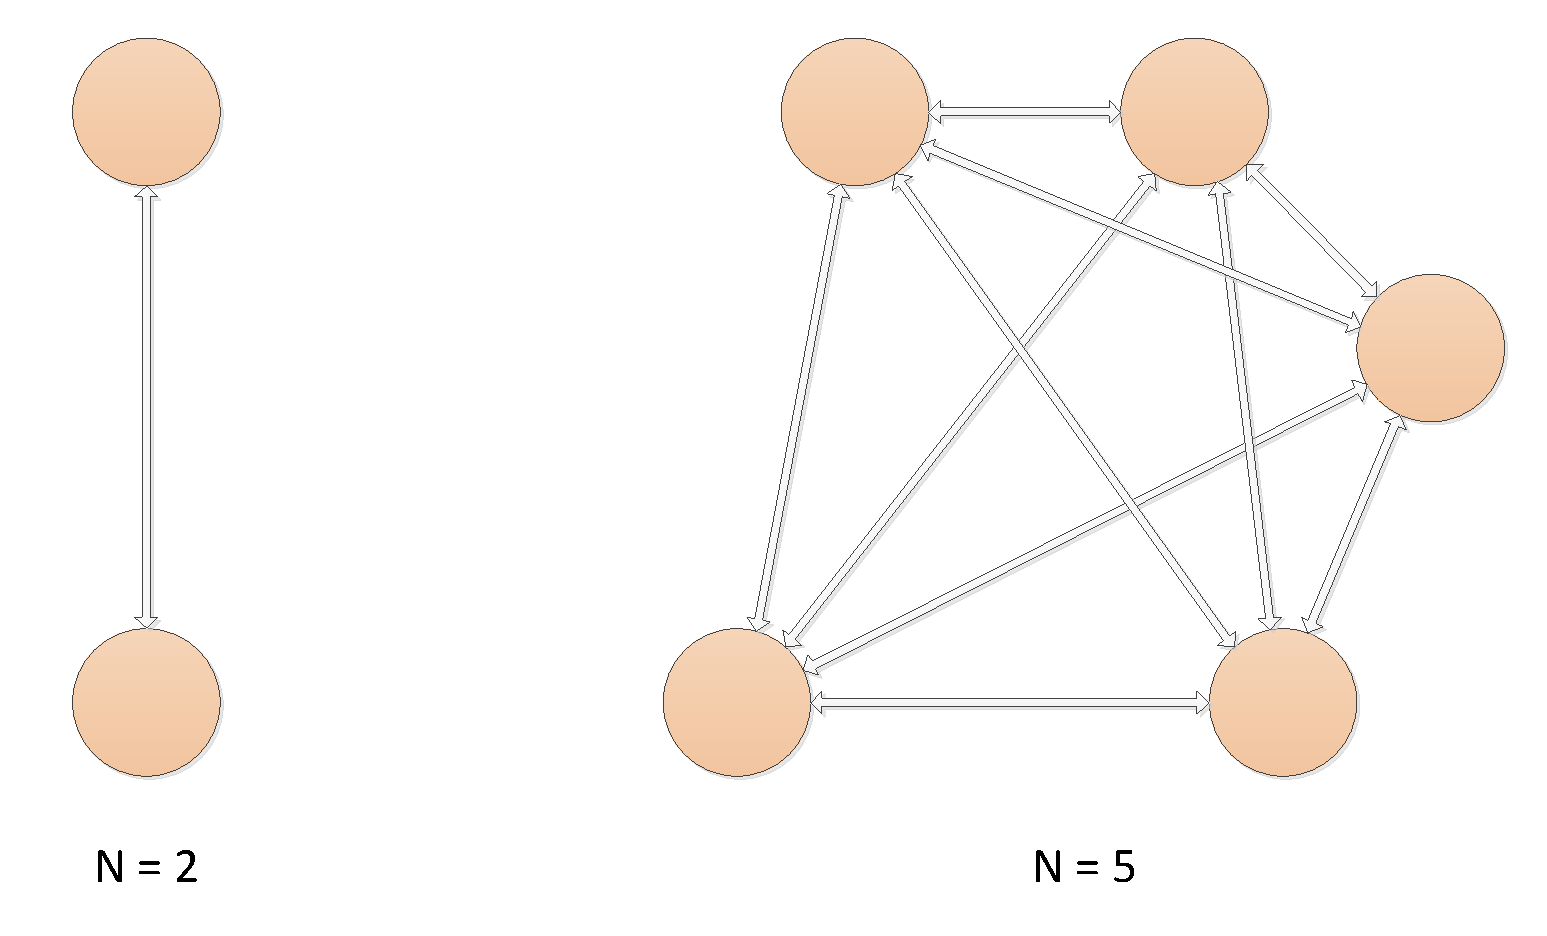
\includegraphics[width=120mm, keepaspectratio]{figures/NBody/N_Body_Alap.pdf}
			\caption{N-test probl�ma kett� �s �t testet tartalmaz� rendszerek eset�ben} 
			\label{fig:N_Body_Alap}
		\end{figure}
	
	%----------------------------------------------------------------------------
	\section{Csillag�szati alkalmaz�s}
	%----------------------------------------------------------------------------
		�gitestek viselked�s�nek le�r�s�val m�r Sir Isaac Newton is foglalkozott, aki sikeresen levezette Kepler t�rv�nyeit, kiindulva a saj�t gravit�ci�s �s mozg�si t�rv�ny�b�l. Kepler felt�telezte, hogy van egy kit�ntetett, fixen elhelyezked� objektum a vil�gegyetemben (Nap), ami k�r�l elliptikus p�ly�n keringenek az �gitestek. Newton a fix �gitest l�tez�s�t elvetette �s bebizony�totta, hogy a Kepler-f�le le�r�s csak egy k�zel�t�st ad a Naprendszer�nk t�nyleges viselked�s�re. Az �gitestek hat�ssal vannak egym�sra, k�lcs�n�sen keringenek egym�s k�r�l. Megj�solta, hogy nem csak elliptikus, hanem parabolikus �s hiperbolikus p�ly�k is el�fordulhatnak~\cite{OrbitMech}.
		
		A jelenlegi mikrohull�m� h�tt�rsug�rz�s egyenletess�ge arra enged k�vetkeztetni, hogy az univerzum anyags�r�s�g szempontj�b�l kezdetben kifejezetten egyenletes volt.
		%...volt: a fluktu�ci� m�rt�ke az �tlagos �rt�kt�l k�r�lbel�l $10^{-4}$ �s $10^{-5}$ nagys�grendbe esett. A m�ra kialakult galaxisok �s a galaxiscsoportok mellett ugyanez az ingadoz�s el�ri ak�r a $10^3$ nagys�grendet is~\cite{CosmSimAnal}.
		A gravit�ci�s k�lcs�nhat�s k�vetkezt�ben az apr� t�m�r�l�sek, csom�k megfelel� kiindul�si pontot biztos�tottak ahhoz, hogy a korai univerzum ,,�sszeomoljon'' �s kialakuljanak jelent�s s�r�s�gbeli elt�r�sek. Az ilyen t�m�r�l�sek n�veked�si, fejl�d�si folyamata �s a k�z�tt�k l�v� kapcsolat is er�sen nemline�ris, ami korl�tozza a tiszt�n analitikus ki�rt�kel�s lehet�s�g�t, el�t�rbe hozva a kor�bban eml�tett numerikus megold�sokat~\cite{CosmSimAnal}.
		
		Az asztrofizik�ban alkalmazott N-test szimul�ci� c�lja, hogy seg�tse meg�rteni az �gitestek, galaxisok �s v�gs� soron az univerzum kialakul�s�t. Szerepet j�tszik p�ld�ul �reszk�z�k, bolyg�k p�ly�j�nak meghat�roz�s�ban, galaxis form�ci�k vizsg�lat�ban �s kiemelked�en fontos m�dszer a s�t�tanyag kutat�s ter�n.

	%----------------------------------------------------------------------------
	\section{�sszef�gg�sek}
	%----------------------------------------------------------------------------
		%----------------------------------------------------------------------------
		\subsection{Test interakci�k}
		%----------------------------------------------------------------------------
			A testek k�zti interakci�t a Newton-f�le gravit�ci�s t�rv�ny seg�ts�g�vel �rhatjuk le, mely szerint b�rmely k�t t�meggel rendelkez� test k�z�tt er�hat�s l�p fel �gy, hogy a testek t�megk�z�ppontj�t egym�s fel� gyors�tja. A kialakul� er� nagys�ga:
			\begin{align}
				F = G\frac{m_{1}m_{2}}{r^{2}}
			\end{align}
			ahol $m_1$ �s $m_2$ a k�t test t�mege, $r$ a k�t test t�megk�z�ppontj�nak t�vols�ga �s $G$ a gravit�ci�s �lland�. A k�pletb�l leolvashat�, hogy a testek k�z�tt hat� er� egyenesen ar�nyos a testek t�meg�vel �s ford�tottan ar�nyos a testek k�zti t�vols�g n�gyzet�vel.

			A gravit�ci�s er� vektori�lis mennyis�g, vagyis ir�nnyal jellemezhet� �s az er� minden esetben a testek t�megk�z�ppontj�nak hat�svonal�ba esik. Vektori�lis alakban a m�sodik test �ltal az els�re kifejtett er�:
			\begin{align}
				\mathbf{F_{12}} = G\frac{m_{1}m_{2}}{\left \| \mathbf{r_{12}} \right \|^{2}}\cdot \frac{\mathbf{r_{12}}}{\left \| \mathbf{r_{12}} \right \|}
			\end{align}
			Itt $\mathbf{r_{12}}$ m�r egy vektort reprezent�l, mely vektor a m�sodik test t�megk�z�ppontj�b�l mutat az els� test t�megk�z�ppontj�ba. Az $\left \| \mathbf{r_{12}} \right \|$ pedig az el�bb eml�tett vektor hossza, vagyis a t�megk�z�ppontok t�vols�ga. A bal oldali t�nyez� az er� nagys�g�t adja meg, m�g a jobb oldali t�nyez� az ir�ny�t, egys�gvektor form�j�ban. Ugyanez fel�rva a m�sodik testre:
			\begin{align}
				\mathbf{F_{21}} = G\frac{m_{1}m_{2}}{\left \| \mathbf{r_{21}} \right \|^{2}}\cdot \frac{\mathbf{r_{21}}}{\left \| \mathbf{r_{21}} \right \|}
			\end{align}
			
			Newton 3. axi�m�ja �rtelm�ben, ha k�t test er�vel hat egym�sra, akkor az az er� mindk�t testre ugyanolyan nagys�g� �s ellent�tes ir�ny�:
			\begin{align}
				\mathbf{F_{12}} = -\mathbf{F_{21}}
			\end{align}
	
			A fenti megfontol�sokat k�vetve az �sszef�gg�sek fel�rhat�k tetsz�leges $N \geq 2$ eg�sz sz�m� objektumra is.
			
			R�t�rve a gravit�ci�s N-test szimul�ci� alap�sszef�gg�seire be kell vezetni n�h�ny jel�l�si konvenci�t, illetve tulajdons�got:

			\begin{itemize}
				\item $\mathbf{F_{ij}}$ a $j.$ test �ltal az $i.$ testre kifejtett gravit�ci�s er�vektor,
				\item $\mathbf{F_{i}}$ az $i.$ testre kifejtett ered� gravit�ci�s er�vektor,
				\item $m_{i}$ az $i.$ test t�mege,
				\item $\mathbf{x_{i}}$ az $i.$ test aktu�lis poz�ci�vektora,
				\item $\mathbf{v_{i}}$ az $i.$ test aktu�lis sebess�gvektora,
				\item $\mathbf{r_{ij}}$ az $j.$ test t�megk�z�ppontj�b�l az $i.$ test t�megk�z�ppontj�ba mutat� vektor, ami $\mathbf{r_{ij}} = \mathbf{x_{j}} - \mathbf{x_{i}}$ alakban �ll el�.
			\end{itemize}
		
			Az indexek mindig egy testet, vagy testeket jel�lnek ki �s �rt�k�k $1 \leq i$ �s $j \leq N$.

			Ezek ut�n az $i.$ testre hat� er�, amit a $j.$ testtel val� gravit�ci�s k�lcs�nhat�s okoz a k�vetkez�k�ppen adhat� meg:
			\begin{align}
				\mathbf{F_{ij}} = G\frac{m_{i}m_{j}}{\left \| \mathbf{r_{ij}} \right \|^{2}}\cdot \frac{\mathbf{r_{ij}}}{\left \| \mathbf{r_{ij}} \right \|}
			\end{align}
			
			Newton 4. axi�m�j�t (az er�hat�sok f�ggetlens�g�nek elv�t) felhaszn�lva, az $i.$ testre hat� ered� er� a rendszerben l�v� m�s testek �ltal okozott er�k vektori�lis �sszegek�nt �rhat� fel:
			\begin{align}
				\mathbf{F_{i}} = \sum_{j = 1,j\neq i}^{N} \mathbf{F_{ij}} = Gm_{i} \sum_{j = 1,j\neq i}^{N} \frac{m_{j}\mathbf{r_{ij}}}{\left \| \mathbf{r_{ij}} \right \|^{3}}
			\end{align}
	
			Amennyiben a testek k�zti t�vols�g tart a null�hoz, a k�zt�k hat� er� tart a v�gtelenhez, ami nem k�v�natos anom�li�khoz vezet a szimul�ci� sor�n. A legt�bb asztrofizikai alkalmaz�sban a testek �tk�z�se tiltott, �gy ezeket a szitu�ci�kat valamilyen form�ban le kell kezelni. Az egyik legegyszer�bb megold�s egy er� enyh�t�s��rt felel�s pozit�v konstans ($\varepsilon^2$ - softening factor) bevezet�se. Seg�ts�g�vel korl�tozni tudjuk a testek k�z�tt kialakul� er� nagys�g�t, ami numerikus integr�l�s sor�n kedvez�. A kieg�sz�tett k�plet:
			\begin{align}
				\mathbf{F_{i}} \approx Gm_{i} \sum_{j = 1}^{N} \frac{m_{j}\mathbf{r_{ij}}}{\left ( \left \| \mathbf{r_{ij}} \right \|^{2} + \varepsilon^{2} \right )^{\frac{3}{2}}}
			\end{align}
			
			A nevez�ben l�v� n�gyzetgy�kvon�s az $r_{ij}$ �s az $\varepsilon$ n�gyzetes �sszegz�se miatt jelenik meg.
			
			Megjegyzend�, hogy a kor�bban feltett $j \neq i$ a tov�bbiakban nem sz�ks�ges, ugyanis $F_{ii}=0$, ha $\varepsilon^2 > 0$. B�r els� r�n�z�sre feleslegesnek t�nik elv�gezni a sz�m�t�sokat $j=i$ esetben, azonban SIMD\footnote{Single Instruction Multiple Data - egy utas�t�s �s t�bb adat (l�sd \figref{Impl_SIMD} �bra).} jelleg� adatfeldolgoz�s eset�n �rdemes elker�lni az el�gaz� utas�t�sokat a hat�konys�g �rdek�ben~\cite{GPUGems}.

		%----------------------------------------------------------------------------
		\subsection{Integr�l�s}\label{sect:NBody_integrateSect}
		%----------------------------------------------------------------------------
			Numerikus integr�l�s sor�n l�p�sr�l-l�p�sre meghat�rozzuk a testek �j poz�ci�j�t �s sebess�g�t a kisz�m�tott er�vel ar�nyos gyorsul�s alapj�n, ezzel szimul�lva az id� halad�s�t. A l�p�sk�z �ltal�ban fix �rt�k�, de a fel�rt egyenletek megoldhat�ak v�ltoz� l�p�sk�z� KDE (k�z�ns�ges differenci�legyenlet) megold� haszn�lat�val is. H�romdimenzi�s esetben minden testhez 6 differenci�legyenlet rendelhet� (3 a poz�ci�-, �s 3 a sebess�gvektor koordin�t�ib�l ad�dik), vagyis az integr�l�s komplexit�sa $O(N)$. Az $i.$ test gyorsul�sa a dinamika alapegyenlete ($a_i = \frac{F_i}{m_i}$)  alapj�n a k�vetkez� m�don alakul:
			\begin{align}
				\label{eq:NBody_accEq}
				\mathbf{a_{i}} \approx G \sum_{j = 1}^{N} \frac{m_{j}\mathbf{r_{ij}}}{\left ( \left \| \mathbf{r_{ij}} \right \|^{2} + \varepsilon^{2} \right )^{\frac{3}{2}}}
			\end{align}
			Numerikus integr�ci� elv�gz�s�re sz�mos lehet�s�g ad�dik. Az egyik legegyszer�bb megold�s az �gynevezett Verlet-m�dszer (Verlet-integrator) haszn�lata. A szimul�ci� sor�n v�lasztott integr�l�si m�dszer befoly�solja mind a sebess�get, mind a pontoss�got, �gy a vizsg�lt probl�ma term�szete nem hagyhat� figyelmen k�v�l a d�nt�s sor�n.
			
			A Verlet-m�dszer gyakran alkalmazott elj�r�s Newton-f�le mozg�segyenletek alkalmaz�s�n�l, valamint objektumok r�pp�ly�j�nak meghat�roz�sa sor�n.
			\begin{align}
				\label{eq:NBody_integrateEq}
				\mathbf{x_{i}}\left ( t + \Delta t \right ) := \mathbf{x_{i}}\left ( t \right ) + \mathbf{v_{i}}\left ( t  \right )\Delta t + \frac{1}{2}\mathbf{a_{i}}\left ( t \right )\Delta t^{2}
			\end{align}
			\begin{align}
				\mathbf{v_{i}}\left ( t + \Delta t \right ) := \mathbf{v_{i}}\left ( t \right ) + \mathbf{a_{i}}\left ( t  \right )\Delta t
			\end{align}
			
			A fentiekb�l l�that�, hogy a l�p�sk�z megv�laszt�s�val �ll�that� a meghat�rozott poz�ci�k �s sebess�g�rt�kek felbont�sa. A l�p�sk�z cs�kkent�s�vel azonban elker�lhetetlen�l n�vekszik a szimul�ci� sor�n elv�gzend� sz�m�t�sok mennyis�ge, �gy a l�p�sk�z helyes megv�laszt�sa mindig kiemelt fontoss�g� feladat.
			
			Ahhoz, hogy a fent levezetett k�pletek haszn�lhat�k legyenek, minden testnek kell rendelkeznie kezdeti felt�telekkel. A szimul�ci� el�tt minden test sz�m�ra megadand� �rt�kek:
			\begin{itemize}
				\item t�meg
				\item poz�ci�vektor
				\item sebess�gvektor
			\end{itemize}
			H�romdimenzi�s t�rben a poz�ci�vektor �s sebess�gvektor h�romelem� vektor, m�g a t�meg skal�ris mennyis�g.
	%----------------------------------------------------------------------------
	\section{Algoritmusok}\label{sect:NBody_algorithmSect}
	%----------------------------------------------------------------------------
		Egy diszkr�t testekb�l �ll� gravit�ci�s rendszer vizsg�latakor sz�ks�ges, hogy minden egyes testre a rendszerben tal�lhat� m�s testek �ltal okozott gyorsul�st meghat�rozzuk.
	
		A direkt algoritmus (brute force) komplexit�sa miatt kifejlesztettek egy�b megold�sokat is, amelyek valamilyen form�ban elhanyagol�sokkal �lnek a gyors v�grehajthat�s�g �rdek�ben.

		Az algoritmus komplexit�s�nak cs�kkent�s�re sz�mos megold�s �ll rendelkez�sre, ezek alapvet�en k�t f� csoportra oszthat�k:

		Az els� csoport a testeket hierarchikus f�ba rendezve t�rolja �s az �gynevezett ,,multipole expansion'' matematikai m�dszerrel k�zel�ti a gravit�ci�s k�lcs�nhat�st. Ilyen algoritmus p�ld�ul a Barnes-Hut vagy a Fast-Multipole m�dszer.
		
		A m�sodik csoport az FFT-t (Gyors Fourier-transzform�ci�) megval�s�t� algoritmusok sebess�g�t igyekszik kihaszn�lni. A testekre hat� gravit�ci�s potenci�lt a h�l� �s a Poisson-egyenlet megold�s�val hat�rozz�k meg. Ilyen p�ld�ul a Particle-mesh (test-h�l�) m�dszer �s annak tov�bbfejlesztett v�ltozatai P3M (Particle-particle-particle-mesh), az AP3M (Adaptive P3M).

		A k�z�s az algoritmusokban, hogy v�dekezni�k kell a valamilyen m�don a ,,k�zeli'' testek k�zti interakci�n�l. Ha az �tk�z�s esete nincs lekezelve a testek egym�st ,,katapultk�nt kil�hetik'' (a Newton-f�le gravit�ci�s t�rv�ny nevez�je nulla k�zeli �rt�k, �s a testek k�z�tt hat� er� v�gtelenhez tart), ami �ltal a szimul�ci� kev�sb� lesz �leth�. A megold�st az �sszef�gg�sek levezet�se sor�n m�r eml�tett k�zeli testek k�zti er� enyh�t�se (force softening) jelenti. Ezt a legegyszer�bben �gy tehetj�k meg, ha a nevez�t kieg�sz�tj�k egy konstans nem nulla �rt�kkel, megakad�lyozva a szingularit�s kialakul�s�t.

		Az N-test szimul�ci�t terhel� hiba meghat�roz�sa nagyon bonyolult feladat. Minden algoritmus t�pus m�sk�nt viselkedik. Az algoritmus fut�si sebess�ge �s a szimul�ci� pontoss�ga egym�ssal ford�tott ar�nyban �ll, �gy az alkalmaz�shoz elengedhetetlen egy sz�munkra megfelel� kompromisszum.
		
		%----------------------------------------------------------------------------
		\subsection{Direkt m�dszer}\label{sect:nbody_direct}
		%----------------------------------------------------------------------------
			A legegyszer�bb �s legk�zenfekv�bb megold�s a sz�m�t�s elv�gz�s�re, ha minden egyes k�lcs�nhat�st kisz�molunk. $N$ darab test eset�n minden egyes test hat a m�sikra, teh�t egy kiszemelt test eset�ben $N - 1$ k�lcs�nhat�st kell kisz�molnunk. �gy �sszess�g�ben $N(N - 1)$ er� kisz�m�t�sa sz�ks�ges egy id�pillanatban. Newton 3. axi�m�ja �rtelm�ben, ha k�t test er�vel hat egym�sra, akkor az az er� mindk�t testre ugyanolyan nagys�g� �s ellent�tes ir�ny�. Ez lehet�s�get biztos�t a sz�ks�ges sz�m�t�sok mennyis�g�nek cs�kkent�s�re. A p�rhuzamos�tott algoritmusok eset�n ez azonban nehezen kihaszn�lhat�, ugyanis sz�ks�gess� teszi az eredetileg egym�st�l f�ggetlen sz�m�t�sokat v�gz� sz�lak k�zti kommunik�ci�t, ami jelent�sen lass�thatja a kalkul�ci�t v�gz� program fut�s�t.

			Az algoritmus komplexit�sa a testek sz�m�val n�gyzetes n�vekszik, �gy ez megfelel� sz�m�t�si kapacit�s hi�ny�ban csak korl�tozott m�rt�kben haszn�lhat� m�dszer.
			
			A direkt m�dszer egy gyorsabb v�ltozata, ha egy bizonyos t�vols�gon t�l, elhanyagoljuk a testek egym�sra hat�s�t. Ez mind�sszesen egy el�gaz�s be�p�t�s�vel megtehet�, �s megsp�rolja a t�ls�gosan kis er�k kisz�m�t�s�t. Ez a legegyszer�bb approxim�ci�, amivel gyors�thatjuk a szimul�ci�t. SIMD eset�n azonban nem nyer�nk vele annyit fut�si sebess�gben, mint amennyit pontoss�gban esetleg vesz�t�nk, ugyanis az egyes sz�laknak ilyen esetben be kell v�rniuk egym�st (lockstep v�grehajt�s). Minden egyes fut� sz�l egy adott pillanatban ugyanazt az utas�t�st hajtja v�gre, ha van sz�m�t�s, ha nincs. �gy ez a gyors�t�si opci� els�sorban az egy sz�lon fut� programok eset�n j�het sz�ba.

		%----------------------------------------------------------------------------
		\subsection{Fa alap� m�dszerek}
		%----------------------------------------------------------------------------	
			A direkt m�dszert �gy pr�b�lj�k k�zel�teni, felgyors�tani, hogy az egym�shoz k�zel l�v� testcsoportokat egy testk�nt kezelik. Ha egy testcsoport kell�en t�vol helyezkedik el az �ppen vizsg�lt testt�l, akkor ennek a csoportnak a gravit�ci�s hat�s�t k�zel�thetj�k a csoport t�megk�z�ppontj�ba helyezett virtu�lis testtel.

			Ezek az algoritmusok felosztj�k a teljes rendelkez�sre �ll� teret cell�kra (k�tdimenzi�s esetben n�gyzet, h�romdimenzi�s esetben kocka). A cell�kat egy bin�ris f�hoz hasonl� m�don t�rolj�k, csak itt a fa egyes elemei 4 (quad-tree), illetve 8 (oct-tree) gyerekkel rendelkeznek dimenzi�t�l f�gg�en~\cite{BHGalSim}.

			A feloszt�s k�tdimenzi�s esetben (quad-tree) az \figref{N_Body_Fa_modszer} �s az \figref{N_Body_Fa_felepites} �br�knak megfelel� m�don addig folytat�dik ameddig egy cella pontosan 1 vagy 0 testet tartalmaz. Ha egy cell�ban t�bb is tal�lhat�, akkor a vizsg�lt cell�t 4 azonos m�ret� kisebb cell�ra bontja. A szeml�ltethet�s�g miatt a k�tdimenzi�s esetet v�lasztottam, de a le�rtak k�nnyed�n alkalmazhat�k h�romdimenzi�s esetben is.

			\begin{figure}[!ht]
			\centering
			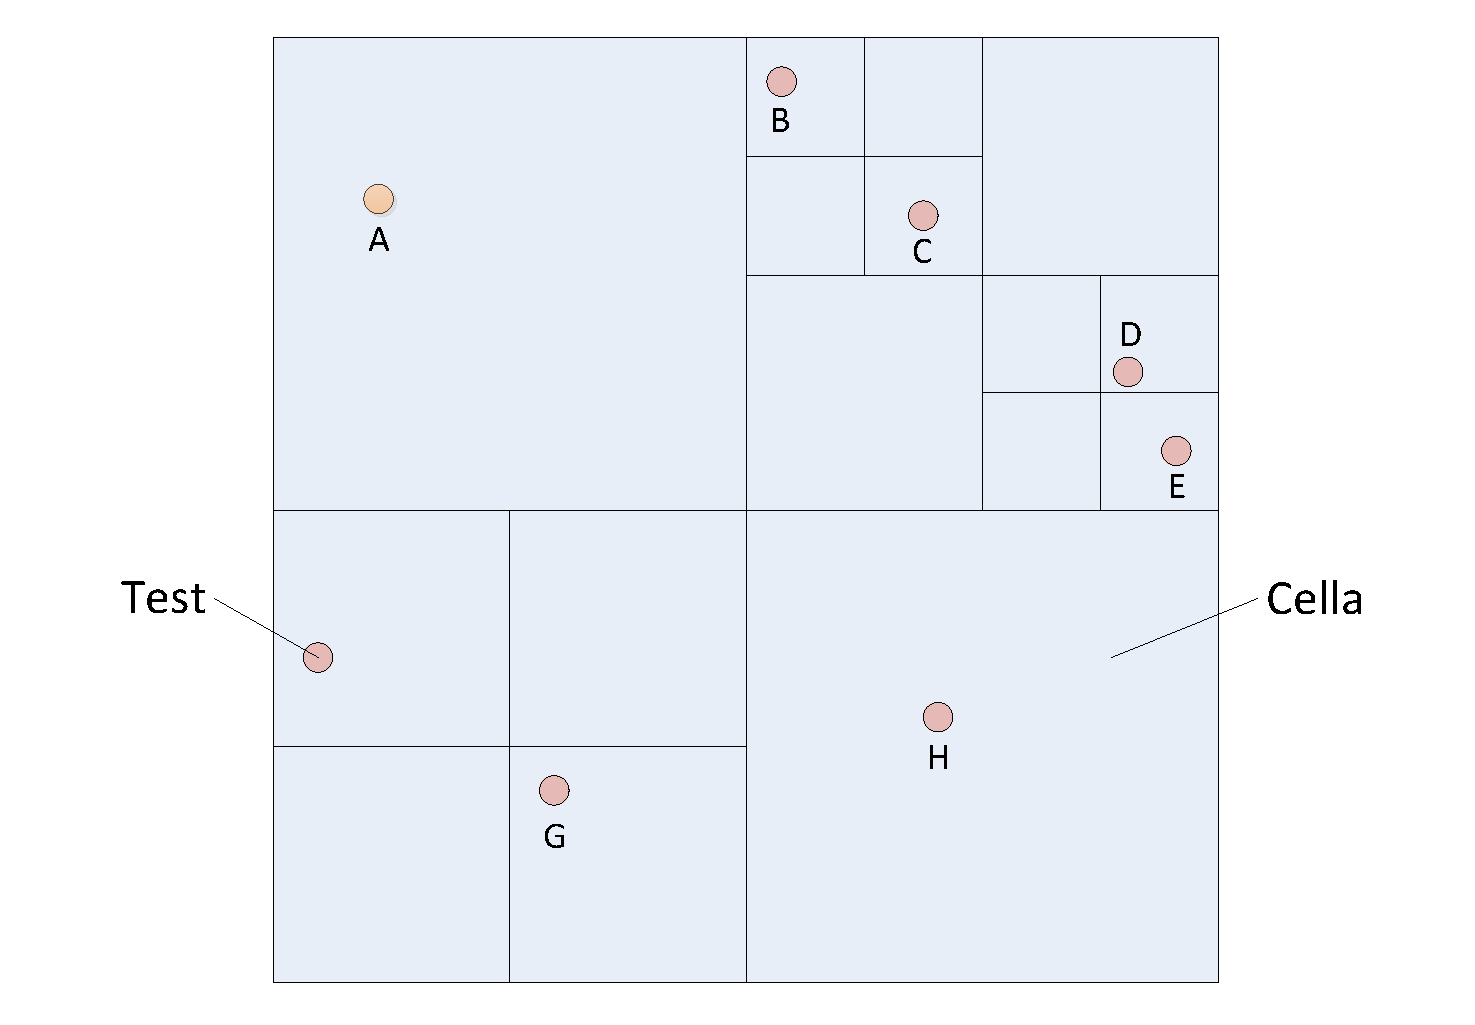
\includegraphics[width=150mm, keepaspectratio]{figures/NBody/N_Body_Fa_modszer.pdf}
			\caption{A cell�kra bontott t�r} 
			\label{fig:N_Body_Fa_modszer}
			\end{figure}
			
			\begin{figure}[!ht]
			\centering
			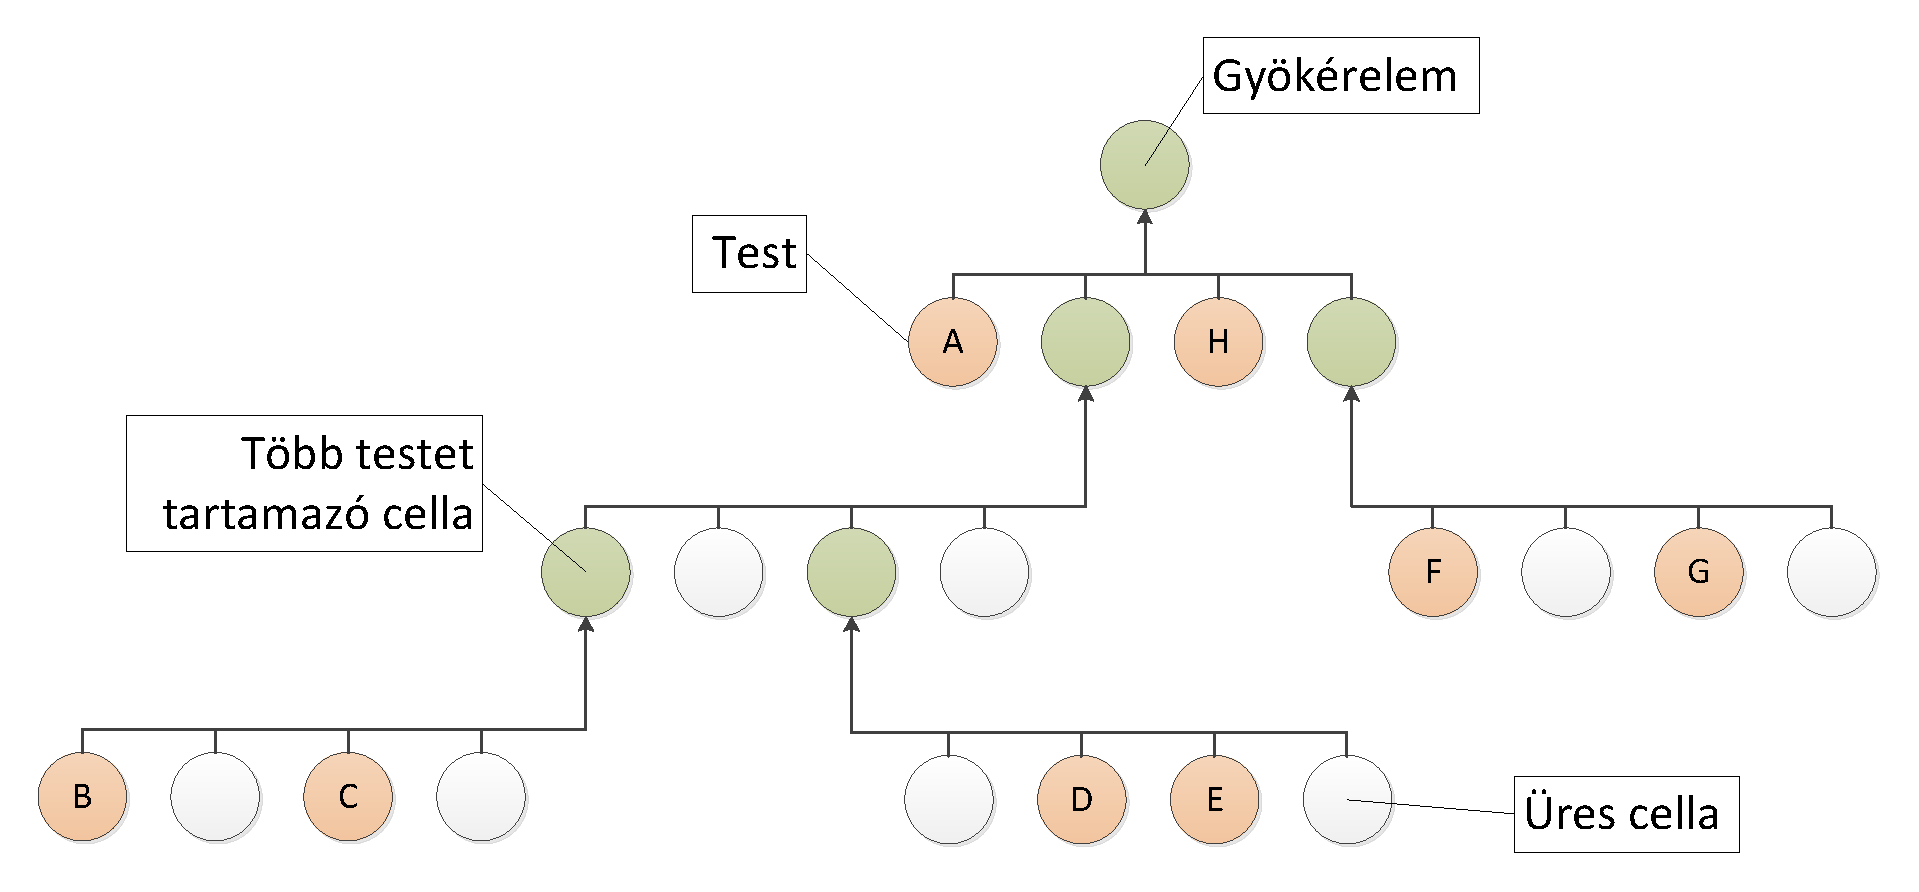
\includegraphics[width=150mm, keepaspectratio]{figures/NBody/N_Body_Fa_felepites.pdf}
			\caption{Az \figref{N_Body_Fa_modszer} �bra alapj�n fel�p�tett fa (quad-tree)} 
			\label{fig:N_Body_Fa_felepites}
			\end{figure}			
			
			A t�bb testet tartalmaz� cell�kat virtu�lis testk�nt kezeli: rendelkeznek t�meggel �s poz�ci�val. A t�meg�k a bennfoglalt testek �sszt�mege, a poz�ci�juk pedig a t�megk�z�ppont.

			Direkt m�dszerhez hasonl�an test-test k�z�tti interakci�kat vizsg�l, belev�ve a virtu�lis testeket is. A f�n fentr�l lefele, balr�l jobbra haladva minden elemet megvizsg�l az algoritmus. Ha �res cell�hoz �r nem tesz semmit, ha testhez, akkor a direkt m�dszerhez hasonl�an kisz�molja a test �ltal okozott er�t. Virtu�lis testhez �rve el�sz�r megvizsg�lja a t�vols�got. Ha a v�geredm�ny az, hogy ,,k�zeli'' a test, akkor a pontoss�g miatt tov�bb megy a rekurzi� a virtu�lis test gyerekeire. Ha azonban ,,kell�en t�voli'' a virtu�lis test a vizsg�lt testt�l, akkor a rekurzi� nem folytat�dik, �s a cell�ban tal�lhat� �sszes testet egy csoportk�nt kezelve ker�l kisz�m�t�sra a gyorsul�s. A felt�tel a ,,kell�en t�volis�gra'':
			\begin{align}
				\frac{s}{d} < \theta 
			\end{align}
			
			ahol $s$ vizsg�lt cella sz�less�ge, $d$ a test �s a cella t�megk�z�ppont t�vols�ga �s $\theta$ pedig egy konstans k�sz�b�rt�k (jellemz�en 0,5).

			A fent bemutatott l�p�ssorozat a Barnes-Hut algoritmust reprezent�lja, melynek komplexit�sa $O(Nlog_{2}N)$. M�s fa alap� m�dszerek is l�teznek, s egyes esetekben ez a komplexit�s reduk�l�dhat ak�r $O(N)$-re is.

		%----------------------------------------------------------------------------
		\subsection{R�szecske-h�l� alap� m�dszerek}
		%----------------------------------------------------------------------------
			Az FFT-t megval�s�t� algoritmusok sebess�g�t kihaszn�l� m�dszerek felosztj�k a teljes teret azonos m�ret� cell�kra (cell), ezzel egy nagy h�l�t (mesh) alkotva �s az �sszes testet (�s azok t�meg�t) hozz�rendelik egy vagy t�bb cell�hoz. A teljes h�l� ezut�n egyfajta test-s�r�s�get reprezent�l, melyre kisz�molva a gravit�ci�s potenci�lt meghat�rozhat�k a testekre hat� er�k, att�l f�gg�en, hogy melyik cell�ban helyezkedik el. A gravit�ci�s potenci�l meghat�roz�s�hoz Poisson egyenlet megold�sa sz�ks�ges~\cite{PartMesh}.
			
			\begin{figure}[!ht]
			\centering
			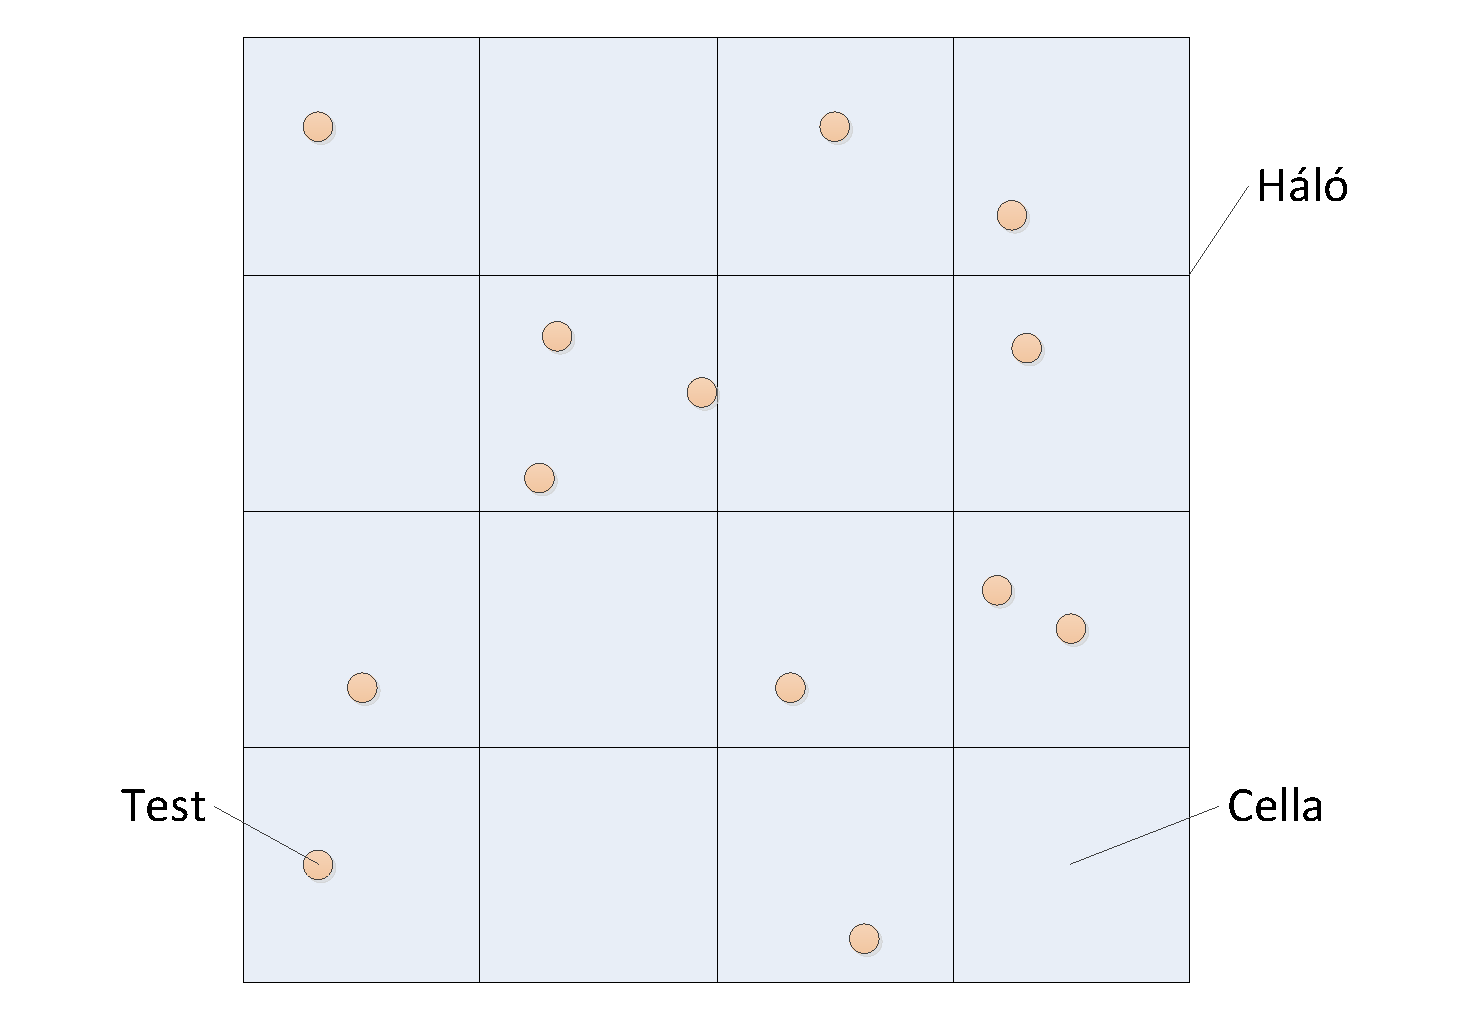
\includegraphics[width=150mm, keepaspectratio]{figures/NBody/N_Body_Particle_Mesh.pdf}
			\caption{Particle-mesh t�pus� algoritmus} 
			\label{fig:N_Body_Particle_Mesh}
			\end{figure}
			
			A Poisson egyenlet a frekvenciatartom�nyban egyszer�bb alakra hozhat� az FFT seg�ts�g�vel.

			A m�dszer el�nyei k�z� tartozik, hogy az algoritmus komplexit�sa $O(N)$, vagyis a sz�m�t�sig�ny �s a testek sz�ma line�ris kapcsolatban vannak. H�tr�nya, hogy a cellam�ret miatt csak v�ges felbont�sra ad lehet�s�get, �s az egym�shoz relat�ve k�zeli testek (t�vols�guk kisebb, mint a cella oldalhossza) k�z�tti er�t nem k�pes modellezni.

			Nagyszab�s� csillag�szati szimul�ci�kban nagyon elterjedt �s kedvelt m�dszercsal�d.
	%----------------------------------------------------------------------------
	\section{Szimul�ci�s hib�k}\label{sect:nbody_szimhibak}
	%----------------------------------------------------------------------------
		Az asztrofizikai N-test rendszerek kaotikusak. M�sk�nt megfogalmazva rendk�v�li �rz�kenys�get mutatnak a kezdeti felt�teleikre (t�meg, poz�ci�, sebess�g), illetve a sz�m�t�sb�l ered� hib�kra. A felt�telekben egy kis elt�r�s is k�pes a szimul�ci� kimenetel�t nagyon megv�ltoztatni.

		Bizony�tott, hogy a sz�m�t�g�pekkel v�gzett szimul�ci�k sor�n keletkez� apr� sz�m�t�si, kerek�t�si hib�k halmoz�d�s�val a kisz�m�tott megold�s exponenci�lisan diverg�l a val�di viselked�st�l, azonos kezdeti felt�telekre. A hiba nagys�ga olyan m�reteket �lthet, hogy ha nem kezelik vagy nem korl�tozz�k valamilyen m�don, az megk�rd�jelezi a szimul�ci� �rv�nyess�g�t.

		K�l�nb�z� N-test szimul�ci�t v�gz� programok �sszehasonl�t�sa sor�n, azonos felt�telek mellett az eredm�nyek $100 \%$-os elt�r�st mutattak. A szimul�ci� kimenetele nagym�rt�kben f�gg a v�lasztott algoritmust�l, annak megval�s�t�s�t�l, illetve a v�lasztott sz�m�t�g�pt�l.

		Bizonyos korl�toz�sok k�z�tt �s meghat�rozott felt�telek mellett a szimul�ci� megb�zhat� eredm�nyt tud adni.

		A hiba n�veked�s�r�l adott r�szletes elm�leti elemz�sek alapj�n, a hib�kat els�sorban az egym�shoz relat�ve k�zeli (t�vols�guk k�zel�t a null�hoz) testek k�z�tti interakci�k okozz�k, �gy a pontoss�g szempontj�b�l az �tk�z�smentes szimul�ci�k kedvez�bbek. A szimul�ci� sor�n fell�p� hib�kat k�t f� csoportba sorolhatjuk~\cite{EffShadow}: 
				
		\begin{itemize}
			\item \textbf{Bemeneti hib�k:} ide tartozik minden modellez�si, k�zel�t�s �s egyszer�s�t�si hiba.
			\begin{itemize}
				\item \textbf{Modellez�si hib�k:}
					\begin{itemize}
						\item \textbf{kvant�l�si hiba/zaj}: a folyamatosnak tekinthet� modellezett rendszer jellemz�se diszkr�t �rt�kekkel.
						\item \textbf{er� korl�toz�sa} (force softening): a k�zeli interakci�kb�l sz�rmaz� er� limit�l�sa.
					\end{itemize}
				\item \textbf{Megval�s�t�si hib�k:}
					\begin{itemize}
						\item \textbf{k�zel�t� algoritmus haszn�lata} (pl.: Barnes-Hut, Fast Multipole m�dszer)
						\item \textbf{numerikus integr�tor v�ges felbont�sa:} integr�l�s helyettes�t�se szumm�z�ssal
						\item \textbf{kerek�t�si hiba}
					\end{itemize}
			\end{itemize}
			\item \textbf{Kimeneti hiba:} a hiba mindig a sz�m�tott �s a val�di k�z�tti elt�r�st mutatja meg. Min�l kisebb ez a hiba ann�l megb�zhat�bb az eredm�ny. Jellemz�en a fent eml�tett bemeneti hib�kb�l k�l�nb�z� s�lyoz�ssal tev�dik �ssze.
		\end{itemize}
		
	%----------------------------------------------------------------------------
	\section{M�rt�kegys�grendszer}
	%----------------------------------------------------------------------------
		Annak �rdek�ben, hogy kezelhet�bb sz�mokkal tudjak dolgozni �gy d�nt�ttem, hogy SI m�rt�kegys�grendszer helyett �tv�ltok csillag�szati m�rt�kegys�grendszerre (IAU - Astronomical System of Units).

		A rendszert az SI-ben val� m�r�sek �s sz�m�br�zol�s okozta neh�zs�gek miatt hat�rozt�k meg, annak �rdek�ben, hogy a nagys�grendeket k�zelebb hozz�k egym�shoz. �sszesen h�rom m�rt�kegys�get defini�l: t�vols�g, t�meg �s id�.

		A t�vols�got csillag�szati egys�gben (astronomical unit) m�rik, r�vid�tve CsE (AU) �s az �ltala defini�lt t�vols�g megegyezik az �tlagos Nap-F�ld t�vols�ggal.

		Az id� alapegys�ge a nap (day), mely 86400 m�sodperck�nt van r�gz�tve. Gyakran haszn�lt egys�g m�g a Juli�n napt�r szerinti �v (year) is mely 365,25 napot tesz ki.

		A t�meget t�bbf�lek�ppen is meg lehet v�lasztani. A hivatalosan elfogadott �rt�k a Nap t�mege, jel�l�se $M_{\odot}$. Alkalmaz�st�l f�gg�en szok�s haszn�lni a Jupiter, vagy a F�ld t�meg�t is. Szimp�tia alapj�n a F�ld t�meg�t v�lasztottam alapegys�gnek.
		\begin{align}
				1~AU = 149~597~870~700~m
		\end{align}
		\begin{align}
				1~D = 86~400~s
		\end{align}
		\begin{align}
				1~M_{\oplus} = 5,9742 \cdot 10^{24}~kg
		\end{align}
		Ennek megfelel�en minden felhaszn�lt konstanst �s sz�rmaztatott mennyis�g �rt�k�t m�dos�tani kell, melyet az alkalmaz�sunk felhaszn�l. Jelen esetben ez csak a gravit�ci�s �lland� �rinti, teh�t �tv�ltva csillag�szati m�rt�kegys�grendszerre:
		\begin{align}
				G = 8,89042279 \cdot 10^{-10} \frac{{AU}^3}{M_{\oplus}D^2}
		\end{align}
%----------------------------------------------------------------------------
\chapter{A dolgozat formai kivitele}
%----------------------------------------------------------------------------
Az itt tal�lhat� inform�ci�k egy r�sze a BME VIK Hallgat�i K�pviselet �ltal k�sz�tett ,,Utols� f�l�v a villanykaron'' c. munk�b�l lett kis v�ltoztat�sokkal �temelve. Az eredeti dokumentum az al�bbi linken �rhet� el: \url{http://vik-hk.bme.hu/diplomafelev-howto-2009}.

%----------------------------------------------------------------------------
\section{A dolgozat kim�rete}
%----------------------------------------------------------------------------
A minim�lis 50, az optim�lis kim�ret 60-70 oldal (f�ggel�kkel egy�tt). A b�r�l�k �s a z�r�vizsga bizotts�g sem szereti kifejezetten a t�l hossz� dolgozatokat, �gy a brutt� 90 oldalt m�r nem �rdemes t�lsz�rnyalni. Egy�bk�nt f�ggetlen�l a dolgozat kim�ret�t�l, ha a dolgozat nem �rdekfesz�t�, akkor az olvas� m�r az elej�n a v�g�t fogja v�rni. �rdemes z�rt, �nmag�ban is �rthet� m�vet alkotni.

%----------------------------------------------------------------------------
\section{A dolgozat nyelve}
%----------------------------------------------------------------------------
Mivel Magyarorsz�gon a hivatalos nyelv a magyar, ez�rt alap�rtelmez�sben magyarul kell meg�rni a dolgozatot. Aki k�lf�ldi posztgradu�lis k�pz�sben akar r�szt venni, nemzetk�zi szint� tudom�nyos kutat�st szeretne v�gezni, vagy multinacion�lis c�gn�l akar elhelyezkedni, annak c�lszer� angolul meg�rnia diplomadolgozat�t. Miel�tt a hallgat� az angol nyelv� verzi� mellett d�nt, er�sen aj�nlott m�rlegelni, hogy ez mennyi t�bbletmunk�t fog a hallgat�nak jelenteni fogalmaz�s �s nyelvhelyess�g ter�n, valamint - nem utols� sorban - hogy ez mennyi t�bbletmunk�t fog jelenteni a konzulens illetve b�r�l� sz�m�ra. Egy nehezen olvashat�, netal�n �rthetetlen sz�veg teher minden j�t�kos sz�m�ra.

%----------------------------------------------------------------------------
\section{A dokumentum nyomdatechnikai kivitele}
%----------------------------------------------------------------------------
A dolgozatot A4-es feh�r lapra nyomtatva, 2,5 centim�teres marg�val (+1~cm k�t�sbeni), 11-12 pontos bet�m�rettel, talpas bet�t�pussal �s m�sfeles sork�zzel c�lszer� elk�sz�teni.



%----------------------------------------------------------------------------
\chapter{Megval�s�t�s}
%----------------------------------------------------------------------------
	Ebben a fejezetben ismertetem az implement�ci� l�p�seit, �s a k�zben felmer�lt probl�m�kat, neh�zs�geket.
	
	A rendelkez�sre �ll� sz�m�t�g�p specifik�ci�ja:

	% Table generated by Excel2LaTeX from sheet 'Specifik�ci�'
	\begin{table}[htbp]
	  \centering
	  \caption{Sz�m�t�g�p specifik�ci�}
		\begin{tabular}{|c|l|l|}
			\hline
			\multicolumn{2}{|l|}{Sz�m�t�g�p m�rk�ja �s t�pusa} & Dell\textregistered~Inspiron\texttrademark~N5110 \\
			\hline \hline
			\multicolumn{2}{|l|}{Kiad�si �v} & 2011 \\
			\hline
			\multicolumn{1}{|l|}{\multirow{6}{*}{Processzor}} & T�pusa & Intel\textregistered~Core\texttrademark~i7-2630QM \\
				  & N�vleges �rajel & $2,00$ GHz \\
				  & Magok sz�ma & $4$ \\
				  & Sz�lak sz�ma & $8$ \\
				  & Utas�t�sk�szlet & $64$ bit \\
				  & Utas�t�sk�szlet kieg�sz�t�s & AVX \\
			\hline
			\multicolumn{1}{|l|}{\multirow{3}{*}{Mem�ria}} & T�pusa & DDR3-1066 MHz \\
				  & M�rete & $8$ GB \\
				  & Maxim�lis s�vsz�less�g & $21,3$ GB/s \\
			\hline
			\multirow{9}{*}{Videok�rtya} & T�pusa & NVIDIA\textregistered~GeForce\texttrademark~525M \\
				  & Architekt�ra & Fermi \\
				  & Magok sz�ma & $96$ \\
				  & N�vleges �rajel & $600$ MHz \\
				  & Elm�leti teljes�tm�ny & $115,2$ GFLOPS \\
				  & Videomem�ria m�ret & $1$ GB \\
				  & Videomem�ria �rajel & $900$ MHz \\
				  & Videomem�ria adatbusz sz�less�g & $128$ bit \\
				  & Elm�leti videomem�ria s�vsz�less�g & $28,8$ GB/s \\
			\hline
		\end{tabular}%
	  \label{tab:szgspecifikacio}%
	\end{table}%

	%----------------------------------------------------------------------------
	%----------------------------------------------------------------------------
\section{MATLAB protot�pus}
%----------------------------------------------------------------------------
	A MATLAB a Mathworks �ltal fejlesztett �s karbantartott programrendszer, mely a MATLAB programoz�si nyelv k�r� �p�l. K�zkedvelt, sz�lesk�r� lehet�s�geket biztos�t els�sorban numerikus sz�m�t�sok �s m�trixm�veletek elv�gz�s�re. Rengeteg be�p�tett f�ggv�ny �s f�ggv�nycsomag mellett tal�lhat� egy grafikus, blokkokb�l �p�tkez� modellez�st �s szimul�ci�t el�seg�t� k�rnyezet is, a Simulink. Elterjedten haszn�lj�k jel- �s adatfeldolgoz�sra, szab�lyoz�tervez�sre, komplex rendszerek (p�ld�ul sz�lturbina) szimul�l�s�ra.
	
	Els� k�rben a gyors megval�s�that�s�g (protot�pustervez�s) �s a rengeteg be�p�tett �br�zol�si lehet�s�g miatt v�lasztottam a MATLAB-ot. M�r fejleszt�s k�zben k�nnyen �szrevehet�v� v�lnak a hib�k.

	Szkriptnyelvr�l l�v�n sz�, ebben az alkalmaz�sban nem a teljes�tm�ny volt a m�rvad�, hanem, hogy megismerkedjek a probl�m�val �s l�ssam, mire kell odafigyelni a k�s�bbi megval�s�t�sok sor�n.

	�rdemes megeml�teni, hogy l�teznek MATLAB sz�m�ra is p�rhuzamos�t�si lehet�s�gek, programcsomagok melyek a sz�m�t�sintenz�v adatfeldolgoz�st hivatottak gyors�tani. Ilyen a Parallel Computing Toolbox, mely magasszint� hozz�f�r�st biztos�t a sz�m�t�g�p er�forr�saihoz, seg�tve a gyors fejleszt�st. Ezzel azonban a diplomamunk�m sor�n nem foglalkoztam.

	A soron k�vetkez� alfejezetekben bemutatom a MATLAB-ban k�sz�tett programom fel�p�t�s�t.

	%----------------------------------------------------------------------------
	\subsection{Main}
	%----------------------------------------------------------------------------
		Az alkalmaz�s egy \verb+Main+ nevezet� script futtat�s�val indul el. A script legelej�n vannak a v�ltoz�k, melyek be�ll�t�s�val v�ltoztathat�k a szimul�ci� param�terei. Ezek szerepenek a \tabref{mat_beallitasok} t�bl�zatban. A jobb olvashat�s�g �rdek�ben csak k�r�l�rom a be�ll�t�sokat �s nem a programban tal�lhat� elnevez�st haszn�lom.
		
		% Table generated by Excel2LaTeX from sheet 'MATLAB t�bl�zat'
		\begin{table}[htbp]
		  \centering
		  \caption{N-test szimul�tor MATLAB v�ltozat�nak konfigur�ci�s lehet�s�gei}
			\begin{tabular}{|l|p{8cm}|}
			\hline
			Be�ll�t�s & Le�r�s \\
			\hline \hline
			Algoritmus t�pus & A v�ltoz�ba el�re defini�lt sztringek �r�s�val v�ltoztathat� az alkalmazott algoritmus. A program jelenleg a direkt m�dszert �s az el�gaz�sos direkt m�dszert val�s�tja csak meg. \\
			\hline
			\multirow{2}[2]{*}{KDE megold� t�pusa �s be�ll�t�sai} & Lehet�s�g van be�p�tett, vagy saj�t (ez l�nyeg�ben az integr�tor) haszn�lat�ra. \\
				  & Be�ll�t�sai csak a be�p�tettnek vannak. \\
			\hline
			Szimul�ci� c�lja �s ciklussz�m & V�laszthatunk egyszeri lefut�s illetve, t�bbsz�ri futtat�s k�z�tt, amivel els�sorban teljes�tm�nym�r�st hajthatunk v�gre. \\
			\hline
			Test param�terek, randomiz�ci� & A testeket inicializ�l� szkript sz�m�ra ad inform�ci�kat. Szint�n itt �ll�that� be a testek sz�ma. \\
			\hline
			Szimul�ci�s id� & A szimul�ci� kezdet�t, v�g�t valamit a l�p�sk�zt tartalmazz�k napokban m�rve. \\
			\hline
			$\varepsilon$ (softening factor) & Csillag�szati egys�gben kifejezett �rt�k, az er�sz�m�t�s sor�n haszn�lja fel a program. \\
			\hline
			Napl�z�s & Lehet�s�g van napl�z�s bekapcsol�s�ra, mely form�zva ki�rja a szimul�ci�s param�tereket, fut�si eredm�nyeket egy sz�veges f�jlba, d�tummal �s id�vel c�mk�zve. \\
			\hline
			\end{tabular}%
		  \label{tab:mat_beallitasok}%
		\end{table}%

		A \verb+Main+ szkript felel�s a t�bbi meg�rt f�ggv�ny megh�v�s��rt. A be�ll�t�sok ut�n el�sz�r az inicializ�ci�s szkript fut le, mely a testeket el�k�sz�ti. Ezt k�vet�en ker�l megh�v�sra maga a szimul�ci�s algoritmus (integr�tor), mely elv�gzi az er�k kisz�m�t�s�t, elmenti a kapott poz�ci��rt�keket a k�s�bbi kijelz�sre �s m�ri a fut�si teljes�tm�nyt.

		A szimul�ci� v�gezt�vel t�rt�nik meg a napl�z�s (amennyiben be van kapcsolva ez az opci�), valamint a fut�si eredm�nyek kijelz�se (teljes fut�si id�, �tlagos fut�si id�, kisz�molt er�k sz�ma m�sodpercenk�nt). A kirajzoltat�s a be�p�tett \verb+plot3()+ f�ggv�nyek seg�ts�g�vel t�rt�nik.

	%----------------------------------------------------------------------------
	\subsection{Inicializ�ci�}
	%----------------------------------------------------------------------------
		A be�ll�t�sok megad�sa ut�n a rendszert inicializ�l� szkript h�v�dik meg, melynek feladata a testek l�trehoz�sa �s a sz�ks�ges kezdeti felt�telek gener�l�sa a be�ll�t�sok alapj�n. A test param�terekben megadhat�k speci�lis sztringek mellyel el�re programozott szimul�ci�k, speci�lis esetek id�zhet�ek el�. Sz�mos �tletem t�madt megval�s�t�s �s tesztel�s k�zben, �m mind�ssze kett�t val�s�tottam meg.

		Az egyik ilyen speci�lis eset a SEL (Sun-Earth-Luna), mely egy $N = 3$ testb�l �ll� rendszert reprezent�l, s kezdeti felt�telei k�zel azonosak a Nap, F�ld �s Hold alkotta h�rmas tulajdons�gaival (t�meg, egym�st�l val� t�vols�g, sebess�g). A \figref{SEL2} ennek fut�s�ra l�thatunk p�ld�t. �sszesen $365$ napot szimul�l a program $1$ napos l�p�sk�zt alkalmazva, a tengelyeken l�that� �rt�kek $AU$-ban �rtend�k. A Nap piros, a F�ld z�ld, a Hold pedig k�k sz�nnel van felt�ntetve. A k�peken a tov�bbiakban a vonal jelzi a megtett utat, a pont vagy kereszt pedig az �ppen aktu�lis poz�ci�t jel�li a t�rben.

		\begin{figure}[!ht]
		\centering
		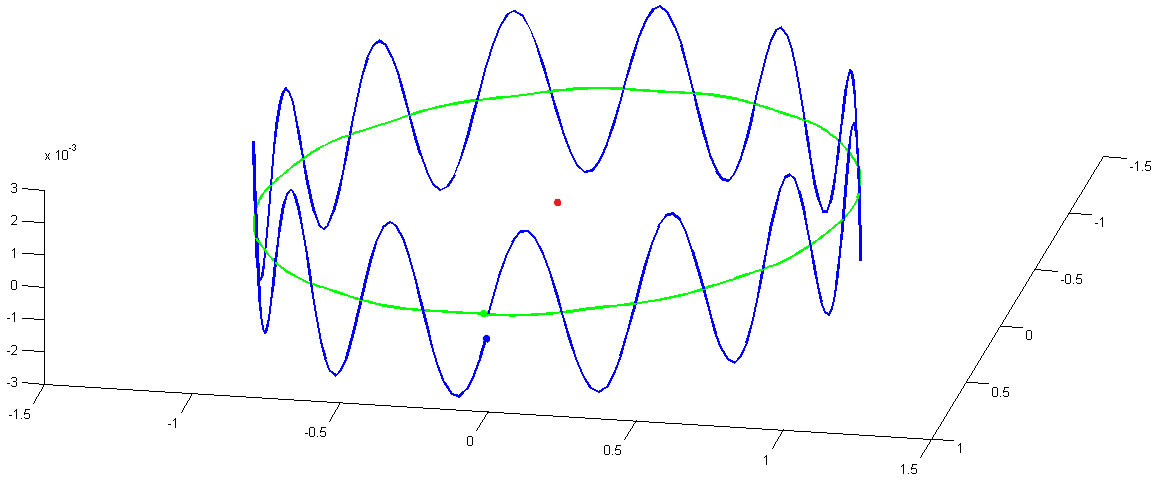
\includegraphics[width=150mm, keepaspectratio]{figures/MATLAB/SEL2.png}
		\caption{Nap-F�ld-Hold h�rmas szimul�ci�ja}
		\label{fig:SEL2}
		\end{figure}
		
		A k�pen sz�pen l�tsz�dik, ahogy a F�ld kering a nap k�r�l, s a Hold �ltal okozott t�megvonz�s miatt apr� kit�r�sek l�that�k a z�ld vonalon. A Nap mozg�sa elhanyagolhat�, �s csak er�sen belenagy�tva l�tsz�dik MATLAB-ban. �rdekes, hogy a Hold �sszesen $13$ peri�dust tesz meg a F�ld k�r�l ($27,3$ nap a kering�si ciklusideje, ami $13$ ciklust jelent $1$ �v alatt). Jelzem, hogy ez egy durva k�zel�t�se a rendszernek �s a be�ll�t�sok m�dos�t�s�val, pontoss�g �ll�t�s�val nagyban v�ltoztathat� a p�lya alakja. Siker�lt olyan szimul�ci�t is futtatni, melyben a Hold p�r �v szimul�ci�ja ut�n ,,belecsap�dott'' a F�ldbe, �gy mindig �rdemes v�giggondolni mennyire helyes a kapott eredm�ny.

		A m�sik megval�s�tott inicializ�ci� sor�n a be�ll�t�sokban megadott \verb+seed+ alapj�n egy el�re defini�lt intervallumon bel�l, v�letlenszer� �rt�kekkel ruh�zza fel a testeket. Az �rt�keket �gy hat�roztam, hogy k�zel re�lisak legyenek, valamint a szimul�ci� sor�n l�tv�nyos eredm�nyt produk�ljanak.
		
		A \figref{16_twister} �br�n egy v�letlenszer� kezdeti felt�telekkel ell�tott, $N = 16$ testb�l �ll� rendszer szimul�ci�ja l�that�. A v�lasztott id�tartam $100~000$ nap, a l�p�sk�z $100$ nap.
		
		\begin{figure}[!ht]
		\centering
		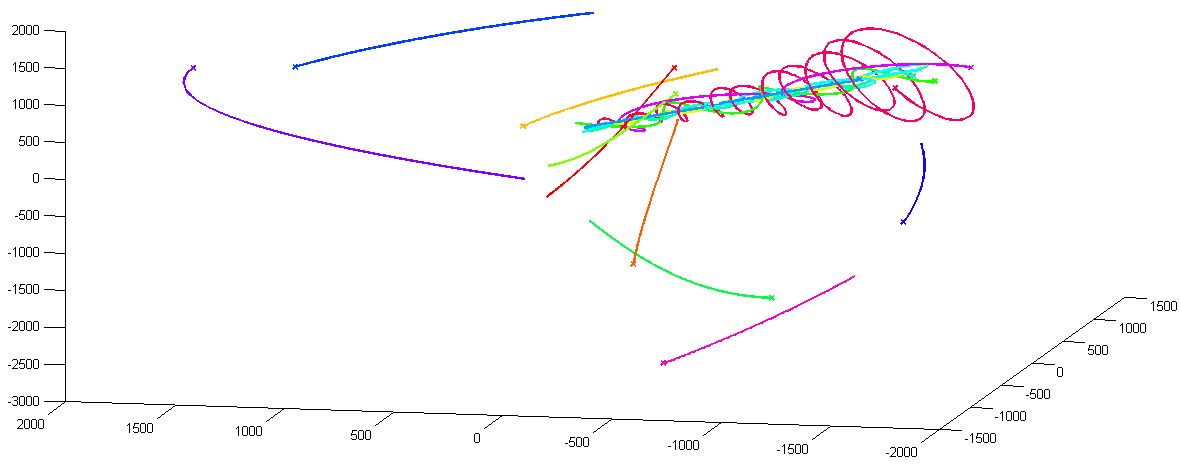
\includegraphics[width=150mm, keepaspectratio]{figures/MATLAB/16_twister.png}
		\caption{N=16 testes szimul�ci�}
		\label{fig:16_twister}
		\end{figure}

		Ennek a szkriptnek a tov�bbfejleszt�si lehet�s�gei k�z� tartozik t�bb speci�lis eset megval�s�t�sa.
		
	%----------------------------------------------------------------------------
	\subsection{Integr�l�s �s az er� sz�m�t�sa}
	%----------------------------------------------------------------------------
		Ebben a csoportban t�bb f�jl (f�ggv�ny) is megtal�lhat�, melyeket egy�tt �rdemes t�rgyalni. Minden algoritmushoz k�t f�jl tartozik. Az egyik egy kieg�sz�t� f�jl, ami az id�m�r�st �s egy�b, kieg�sz�t� teend�ket l�t el, valamint az ezekb�l a f�ggv�nyekb�l megh�v�sra ker�l�, algoritmust megval�s�t� integr�torok, amik az er� kisz�m�t�s�t v�gzik a megadott id�intervallumon bel�l, a megadott be�ll�t�sok szerint.

		�sszesen h�rom ilyen f�jlp�rt val�s�tottam meg, melyek a Main szkriptb�l megh�vhat�k:
		\begin{enumerate}
			\item Direkt m�dszer, saj�t integr�torral
			\item Direkt m�dszer, be�p�tett KDE megold� seg�ts�g�vel
			\item K�zel�tett direkt m�dszer, saj�t integr�torral
		\end{enumerate}

		A be�p�tett KDE megold� lecser�lhet�. Jelenleg az \verb+ode45+ nev�t haszn�lja, ami egy Runge-Kutta m�dszert megval�s�t�, v�ltoz� l�p�sk�z� algoritmuson alapszik. A l�p�sk�z mindig a jelv�ltoz�s (eset�nkben a poz�ci�, sebess�g) m�rt�ke adja meg. Min�l intenz�vebb a p�lyav�ltoz�s ann�l s�r�bb a ki�rt�kel�sek sz�ma, ezzel seg�ti optim�lis sebess�g-pontoss�g ar�ny el�r�s�t.
		
	%----------------------------------------------------------------------------
	\subsection{Eredm�nyek}
	%----------------------------------------------------------------------------
		Egy p�lda szimul�ci�n kereszt�l mutatom be a fut�si eredm�nyeket �s az eredm�nybeli elt�r�seket. A relev�ns be�ll�t�sokat \tabref{mat_eredmenybellitasok}, a fut�si id�ket pedig a \tabref{mat_futasieredmenyek} t�bl�zat tartalmazza.
		
		% Table generated by Excel2LaTeX from sheet 'MATLAB eredm�nyek'
		\begin{table}[htbp]
		  \centering
		  \caption{Futtat�si be�ll�t�sok}
			\begin{tabular}{|l|p{8cm}|}
			\hline
			Be�ll�t�s & �rt�k \\
			\hline \hline
			Testek sz�ma & $32$ \\
			\hline
			Testek tulajdons�gai & V�letlenszer� (mivel a \verb+Seed+ mindig azonos, ez�rt a gener�lt kezdeti �rt�kek is azonosak) \\
			\hline
			Szimul�ci� id�tartama & $20000$ \\
			\hline
			Szimul�ci�s l�p�sk�z & $100$ \\
			\hline
			$\varepsilon$ (softening factor) & $1$ \\
			\hline
			Seed  & $10$ \\
			\hline
			\end{tabular}%
		  \label{tab:mat_eredmenybellitasok}%
		\end{table}%

		% Table generated by Excel2LaTeX from sheet 'MATLAB eredm�nyek'
		\begin{table}[htbp]
		  \centering
		  \caption{Program fut�si id�k}
			\begin{tabular}{|l|l|l|}
			\hline
			M�dszer & Megold� & �tlagos fut�si id� [sec] \\
			\hline \hline
			Direkt & Saj�t integr�tor & $0,7013$ \\
			\hline
			Direkt & \verb+ode45+ KDE megold� & $12,959$ \\
			\hline
			K�zel�tett direkt & Saj�t integr�tor & $0,2853$ \\
			\hline
			\end{tabular}%
		  \label{tab:mat_futasieredmenyek}%
		\end{table}%

		A szeml�letes grafikus bemutat�s miatt v�lasztottam a testsz�mot $32$-re. A teljes keletkezett �br�k a \todo f�ggel�kben tal�lhat�k.

		A fut�si sebess�gb�l l�tszik, hogy a saj�t integr�tor �s a KDE megold� �sszehasonl�t�sa neh�z feladat, mivel a KDE implement�ci�ja sz�momra ismeretlen, �s a be�ll�tott hibaparam�terek, ami alapj�n dolgozik, nagyban befoly�solj�k a v�geredm�nyt. El�fordult olyan helyzet, amikor l�nyegesen gyorsabb volt, mint a saj�t megval�s�t�som, de el�fordult olyan is, hogy szingularit�s miatt hiba�zenettel fejezte be a fut�st. A k�zel�t� m�dszer a v�rt m�don felgyors�totta a fut�st, jelen esetben a szorz� k�zel $2,5$.

		A f�ggel�kben l�v� �br�kon l�that�k elt�r�sek, melyek az apr� akkumul�l�dott hib�knak �s az elt�r� implement�ci�nak tudhat� be. Ez egy p�lda arra vonatkoz�an, hogy a k�l�nb�z� N-test szimul�ci�t megval�s�t� alkalmaz�sok korrekt �sszehasonl�t�sa mennyire neh�zkes feladat a megval�s�t�s ismeret�nek hi�ny�ban.
		
	%----------------------------------------------------------------------------
	\subsection{Konkl�zi�}
	%----------------------------------------------------------------------------
		Sz�mos, k�l�nb�z� kezdeti felt�tellel elv�gzett szimul�ci� ut�n n�h�ny fontos dolgot megtapasztaltam.

		El�sz�r is a \emph{kezdeti felt�telek} nagyon fontosak. Ha egy test sebess�g�t, egy adott t�vols�gn�l megfelel�en �ll�tom be el�rhet�ek stabil kering�si p�ly�k (p�ld�ul kett� test eset�n). Azonban ha kisebbre veszem, akkor �tk�znek. Ha nagyobbra, akkor a k�zt�k kialakul� er�k hat�sa eleny�sz� lesz �s t�volodni fognak egym�st�l v�gig. L�sd \sectref{nbody_szimhibak} alfejezet.

		M�sik fontos probl�ma a \emph{numerikus szingularit�s}. Ha a k�t test nagyon megk�zel�ti egym�st �s v�gs� esetben egym�son lesznek, a kialakul� er� k�zel v�gtelen nagy lehet, ami jelen esetben azt eredm�nyezte, hogy kil�tt�k egym�st ellent�tes ir�nyban.

		Harmadik probl�ma az \emph{integr�ci�s id� probl�m�ja}. Ha t�l nagy l�p�sk�zt v�lasztok az egyenletek kisz�m�t�sa k�z�tt, akkor nagyon pontatlan eredm�nyt kapok ugyanazon kezdeti felt�telekre, esetekben felismerhetetlen�l nagy elt�r�sekkel.

	
	%----------------------------------------------------------------------------
\section{C++ implement�ci�}
%----------------------------------------------------------------------------
	GPU programoz�sn�l a C �s C++ programoz�si nyelvek a legt�mogatottabbak; relat�ve alacsonyszint�ek �s j� teljes�tm�ny �rhet� el vel�k. A szimul�tor meg�r�s�hoz mindenk�ppen objektumorient�lt nyelvet szerettem volna alkalmazni, �gy a C++-ra esett a v�laszt�som.

	A szimul�torral kapcsolatban kit�z�tt kezdeti c�lok nagy vonalakban:
	
	\begin{itemize}
		\item Legyen k�nnyen karbantarthat�, az implement�lt oszt�lyhierarchia legyen nyitott a k�s�bbi kieg�sz�t�sekre �s m�dos�t�sokra.
		\item Min�l jobb p�rhuzamos�t�si eredm�ny el�r�se.
		\item Futtat�si param�terek (konfigur�ci�) legyenek a felhaszn�l� �ltal, �jraford�t�s n�lk�l �ll�that�k.
		\item Egy sz�lon fut� referenciamodell biztos�t�sa az eredm�nyek sz�mszer� ellen�rz�s�hez.
		\item Grafikus megjelen�t�s az ellen�rz�shez.
		\item Sz�m�t�si teljes�tm�ny m�r�se �s kijelz�se.
	\end{itemize}

	Megfelel� grafikai ismeret h�j�n, egy viszonylag egyszer� megjelen�t�st szerettem volna l�trehozni. A rendelkez�sre �ll� seg�danyag, illetve aj�nl�sok alapj�n az \emph{OpenGL}-t (Open Graphics Library) v�lasztottam.

	Az egyszer�bb bemutathat�s�g �rdek�ben feldaraboltam a programom oszt�lyszerkezet�t h�rom logikailag egybef�gg� csoportra. Az oszt�lyokat tartalmaz� �br�kon a tagv�ltoz�k �s a tagf�ggv�nyek csak r�szlegesen vannak felt�ntetve, valamint az �tl�that�s�g �rdek�ben a f�ggv�ny argumentumlist�k �resek. A fejezetnek nem c�lja, hogy r�szletess�g�ben fel�rjen egy teljes �rt�k� dokument�ci�val.

	Az osz�lyokat �s strukt�r�kat egy \verb+NBody+ prefixummal l�ttam el, valamint az oszt�ly tagv�ltoz�k nev�ben haszn�ltam kieg�sz�t� jel�l�seket:
	
	\begin{itemize}
		\item \verb+m+ - tagv�ltoz� (member)
		\item \verb+p+ - mutat� (pointer)
		\item \verb+h+ - host
		\item \verb+d+ - eszk�z (device)
	\end{itemize}

	�gy p�ld�ul az \verb+mpd_position+ egy, az eszk�z mem�ri�j�ban allok�lt c�mre mutat� tagv�ltoz� pointer.

	Az oszt�lyokb�l rendszerint egy-egy p�ld�ny l�tezik a szimul�tor fut�sa sor�n, �gy gyakran egyszer�en csak oszt�lyn�vvel fogok hivatkozni r�juk, a t�nyleges objektum megnevez�se n�lk�l.
	
	%----------------------------------------------------------------------------
	\subsection{Konfigur�ci�s param�terek}
	%----------------------------------------------------------------------------
		Az \figref{Impl_Properties} �br�n l�that� diagram mutatja a csoportnak a fel�p�t�s�t. F�leg enumer�ci�kat, valamint egy strukt�r�t tartalmaz, melynek feladata a felhaszn�l� �ltal be�ll�tott param�terek t�rol�sa. A param�tereket a program futtat�sakor adhatja meg a felhaszn�l� kulcs-�rt�k ($key=value$) form�ban.
		
		\begin{figure}[!ht]
		\centering
		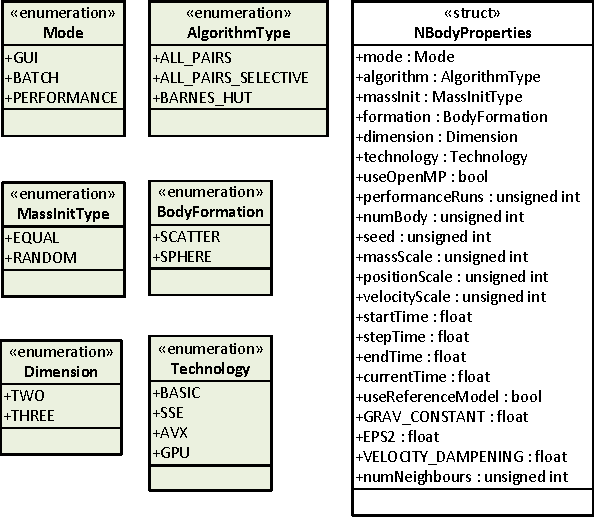
\includegraphics[width=150mm, keepaspectratio]{figures/Implementation/Impl_Properties-cropped.pdf}
		\caption{Futtat�si be�ll�t�sokat t�rol� strukt�ra �s kieg�sz�t� enumer�ci�i}
		\label{fig:Impl_Properties}
		\end{figure}

		A rendszerben tal�lhat� t�bbi oszt�ly rendelkezik \verb+NBodyProperties+ t�pus� tagv�ltoz�val, ami egy k�z�s, a main f�ggv�ny elej�n felt�lt�tt objektumra mutat. A strukt�ra egyes attrib�tumait �s szerep�ket az \tabref{Impl_propertiesTable} t�bl�zat ismerteti r�viden.

		% Table generated by Excel2LaTeX from sheet 'NBodyProperties'
		\begin{table}
		  \centering
		  \caption{Be�ll�that� param�terek �s r�vid bemutat�suk}
			\begin{tabular}{|l|p{93mm}|}
			\hline
			Attrib�tum & Le�r�s \\
			\hline \hline
			mode  & Program felhaszn�l�s�nak szempontj�b�l a legalapvet�bb be�ll�t�s, mellyel megadhat�, hogy grafikus kijelz�st vagy teljes�tm�nym�r�st szeretn�nk v�gezni a futtat�s sor�n.  \\
			\hline
			algorithm & Az algoritmus t�pus�t v�laszthatjuk ki. Jelenleg csak ALL\_PAIRS opci� a t�mogatott, mely az \sectref{nbody_direct} fejezetben bemutatott direkt m�dszernek felel meg. \\
			\hline
			massInit & V�letlenszer� vagy azonos t�meg� testek gener�l�sa. \\
			\hline
			formation & A testek kezdeti poz�ci�j�t befoly�sol� be�ll�t�s, mellyel megadhat�, hogy az �sszes test a orig� k�r�l vagy pedig sz�tsz�rtan, csoportokban helyezkedjenek el. \\
			\hline
			dimension & A testek poz�ci�j�nak harmadik koordin�t�j�t lehet vele fixen kinull�zni. \\
			\hline
			technology & Egy m�sik fontos be�ll�t�s, mellyel megadhatjuk az alkalmazand� p�rhuzamos�t�si technik�t. Lehet v�lasztani a tiszt�n C++ alap� vagy SSE, AVX vektorutas�t�sokat alkalmaz�, illetve GPU-s megval�s�t�s k�z�tt. \\
			\hline
			useOpenMP & OpenMP alap� t�bbsz�l�s�t�s alkalmaz�sa CPU-s algoritmusok eset�n. \\
			\hline
			performanceRuns & Teljes�tm�ny m�r�s sor�n a teljes szimul�ci� lefuttat�s�nak sz�ma. A fut�si eredm�ny ennek f�ggv�ny�ben ker�l ki�tlagol�sra. \\
			\hline
			numBody & A testek sz�ma. SSE �s AVX haszn�lata mellett a 4, illetve 8-al oszthat� darabsz�m a prefer�lt. \\
			\hline
			seed  & A testek kezdeti param�tereit megad� v�letlensz�m gener�tor magja. Azonos konfigur�ci� haszn�lata reproduk�lhat�v� teszi a szimul�ci�kat. \\
			\hline
			massScale & A testek t�meg�t befoly�sol� t�nyez�. Ek�r�l a sz�m k�r�l ker�lnek az �rt�kek gener�l�sra. \\
			\hline
			positionScale & A testek kezdeti poz�ci�j�t befoly�sol� t�nyez�. Ek�r�l a sz�m k�r�l ker�lnek az �rt�kek gener�l�sra. \\
			\hline
			velocityScale & A testek kezdeti sebess�g�t befoly�sol� t�nyez�. Ek�r�l a sz�m k�r�l ker�lnek az �rt�kek gener�l�sra. \\
			%\hline
			%initVelocityFactor & Nem relev�ns. M�sodlagos sk�l�z�s a testek kezdeti sebess�g�re. \\
			\hline
			startTime & Szimul�ci� kezd�s id�pontja. Jelenleg nem sok mindent befoly�sol. Tipikusan 0 �rt�k�. \\
			\hline
			stepTime & Szimul�ci�s l�p�sk�z. �j poz�ci�- �s sebess�g�rt�kek meghat�roz�s�n�l van fontos szerepe. \\
			\hline
			endTime & A szimul�ci� v�gid�pontja. A startTime �s a stepTime seg�ts�g�vel kalkul�l�dik ki a szimul�ci�s iter�ci�k sz�ma. \\
			\hline
			currentTime & A jelenlegi szimul�ci�s id�t tartalmaz� v�ltoz�. \\
			%\hline
			%allowLogger & Nem relev�ns. Tervben volt, a fut�si eredm�nyeket egy sz�veges log f�jlba ki�r� oszt�ly l�trehoz�sa. Ezzel a param�terrel lehetett volna ki-bekapcsolni. \\
			\hline
			useReferenceModel & Egy sz�lon fut� referencia algoritmus haszn�lat�t �s a testek poz�ci��rt�keinek �sszehasonl�t�s�t lehet vele bekapcsolni. \\
			\hline
			GRAV\_CONSTANT & Gravit�ci�s konstans. \\
			\hline
			EPS2  & $\varepsilon^2$ - softening factor. \\
			\hline
			VELOCITY\_DAMPENING & Integr�l�s sor�n, a sebess�g�rt�kek sz�m�t�sakor bej�v� szorz�t�nyez�. \\
			\hline
			\end{tabular}%
		  \label{tab:Impl_propertiesTable}%
		\end{table}%

	%----------------------------------------------------------------------------
	\subsection{Algoritmusok}
	%----------------------------------------------------------------------------
		Az algoritmusokhoz megval�s�t� oszt�lyokat �s a k�zt�k l�v� kapcsolatokat a \figref{Impl_Algorithm} �bra szeml�lteti.

		\begin{figure}[!ht]
		\centering
		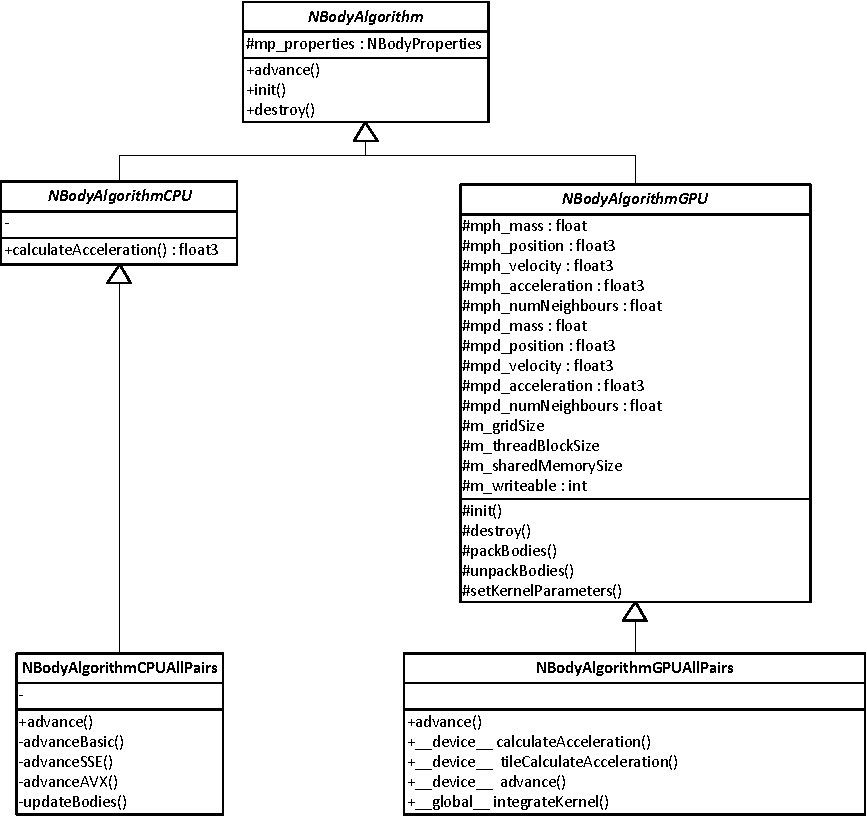
\includegraphics[width=150mm, keepaspectratio]{figures/Implementation/Impl_Algorithm-cropped.pdf}
		\caption{Az algoritmusokhoz kapcsol�d� oszt�lyok}
		\label{fig:Impl_Algorithm}
		\end{figure}

		Strategy tervez�si mint�t (design pattern) alkalmaztam, hogy az egyes algoritmusok cser�lhet�k legyenek a program t�bbi r�sz�nek befoly�sol�sa n�lk�l. Az algoritmust p�ld�nyos�t� oszt�ly sz�m�ra k�z�mb�sek a megval�s�t�s r�szletei.
		%----------------------------------------------------------------------------
		\subsubsection{NBodyAlgorithm}
		%----------------------------------------------------------------------------
			Egy absztrakt �soszt�ly, mely az egys�ges interf�sz szerep�t t�lti be. A program szimul�ci��rt felel�s oszt�lya egy ilyen t�pus� pointerrel rendelkezik, ami t�nylegesen egy tagf�ggv�ny implement�ci�kat m�r tartalmaz�, lesz�rmazott oszt�ly egy objektum�ra mutat.
			
			Az \verb+advance+ met�dus megh�v�s�val minden testre kisz�m�t�sra ker�lnek az �j gyorsul�s�rt�kek, valamint ezek f�ggv�ny�ben friss�l a poz�ci�- �s a sebess�gvektor is. A program fut�sa sor�n ebben a met�dusban t�lti el a legt�bb id�t.
			
			Az \verb+init+ �s a \verb+destroy+ tagf�ggv�nyek az eszk�z mem�riater�let�nek allok�ci�j�t, valamint felszabad�t�s�t v�gzik.
		
		%----------------------------------------------------------------------------
		\subsubsection{NBodyAlgorithmCPU}
		%----------------------------------------------------------------------------
			Szint�n egy absztrakt oszt�ly, mely a testp�rok~~k�z�tti gyorsul�s�rt�keket~~kisz�m�t� \verb+calculateAcceleration+ tagf�ggv�nyek defin�ci�it tartalmazza. K�t test k�z�tti interakci� m�rt�k�nek kisz�m�t�sa ugyanis teljes eg�sz�ben algoritmus f�ggetlen.
			
			Az~~\figref{Impl_Algorithm}~~�br�n~~csak~~egy~~met�dust~~jel�ltem~~meg,~~azonban~~t�nylegesen~~6 \verb+calculateAcceleration+ ker�lt megval�s�t�sra. Ebb�l 3 a teljes�tm�nym�r�shez, 3 pedig a grafikus kijelz�shez haszn�latos; 1-1 sor plusz k�dot (szomsz�dok sz�m�nak meghat�roz�sa) �s argumentumlist�t lesz�m�tva p�ronk�nt azonosak. A h�rom tagf�ggv�nyp�rb�l kett� haszn�l speci�lis p�rhuzamos�t�si technik�kat, a harmadik nat�v C++ referenciaf�ggv�ny. Sima C++ megval�s�t�s eset�n 1, SSE eset�n egyszerre 4, AVX eset�n pedig egyszerre 8 gyorsul�s�rt�k ker�l kisz�m�t�sra.
			
			A k�l�nb�z� N-test algoritmus implement�ci�k ebb�l az oszt�lyb�l sz�rmaznak le. A k�vetkez� l�p�s lehetne egy \verb+NBodyAlgorithmCPUBarnesHut+ oszt�ly megval�s�t�sa p�ld�ul.

		%----------------------------------------------------------------------------
		\subsubsection{NBodyAlgorithmCPUAllPairs}
		%----------------------------------------------------------------------------
			Ez az \sectref{nbody_direct} fejezetben bemutatott direkt m�dszert megval�s�t� oszt�ly. A futtat�si be�ll�t�sokt�l f�gg�en, ciklikusan meg kell h�vnia a megfelel�, az �soszt�lyban implement�lt \verb+calculateAcceleration+ met�dust. Miut�n minden testre kisz�molta az �j gyorsul�s�rt�keket, j�n az integr�l�s, vagyis a poz�ci�- �s sebess�g�rt�kek friss�t�se (\verb+updateBodies+ tagf�ggv�ny).

		%----------------------------------------------------------------------------
		\subsubsection{NBodyAlgorithmGPU}
		%----------------------------------------------------------------------------
			Hasonl� feladatot t�lt be, mint a CPU-s t�rsa, csak kieg�sz�l GPU-s futtat�shoz sz�ks�ges pointerekkel �s met�dusokkal. Az algoritmus p�ld�nyos�t�sakor lefut� \verb+init+ met�dus fogja az eszk�z mem�ri�j�ban a sz�ks�ges ter�leteket lefoglalni, valamint a kezdeti �rt�keket bem�solni. L�nyeges elt�r�s a CPU-s megval�s�t�st�l, hogy a jobb teljes�tm�ny el�r�s �s optim�lisabb mem�riahaszn�t �rdek�ben t�mb�kbe ,,kicsomagolt'' testekkel dolgozik, a \figref{Impl_System} �br�n l�that� a \verb+Body+ nev� strukt�ra helyett. A \verb+packBodies+, �s az \verb+unpackBodies+ tagf�ggv�nyek v�gzik az adatok m�sol�s�t egyik form�b�l a m�sikba. Ezeknek csak grafikus megjelen�t�s eset�n van szerep�k.

		%----------------------------------------------------------------------------
		\subsubsection{NBodyAlgorithmGPUAllPairs}
		%----------------------------------------------------------------------------
			Szint�n a direkt N-test algoritmust val�s�tja meg az oszt�ly, csak most GPU a c�leszk�z. Bizonyos f�ggv�nyeket szerettem volna az �soszt�ly�ba be�gyazni, de a ford�t� valamilyen okn�l fogva ezt nem engedte, �gy itt ker�lt minden kernel �s hozz�tartoz� seg�df�ggv�ny implement�l�sra. Az \verb+integrateKernel+ egyszeri megh�v�s�val t�rt�nik egy szimul�ci�s iter�ci� lefuttat�sa.
		
	%----------------------------------------------------------------------------
	\subsection{Rendszer}
	%----------------------------------------------------------------------------
		Ez az oszt�lycsoport alkotja a szimul�tor k�zponti r�sz�t. Az oszt�lyok k�z�tti kapcsolatot modellezi a \figref{Impl_System} �bra.

		\begin{figure}[!ht]
		\centering
		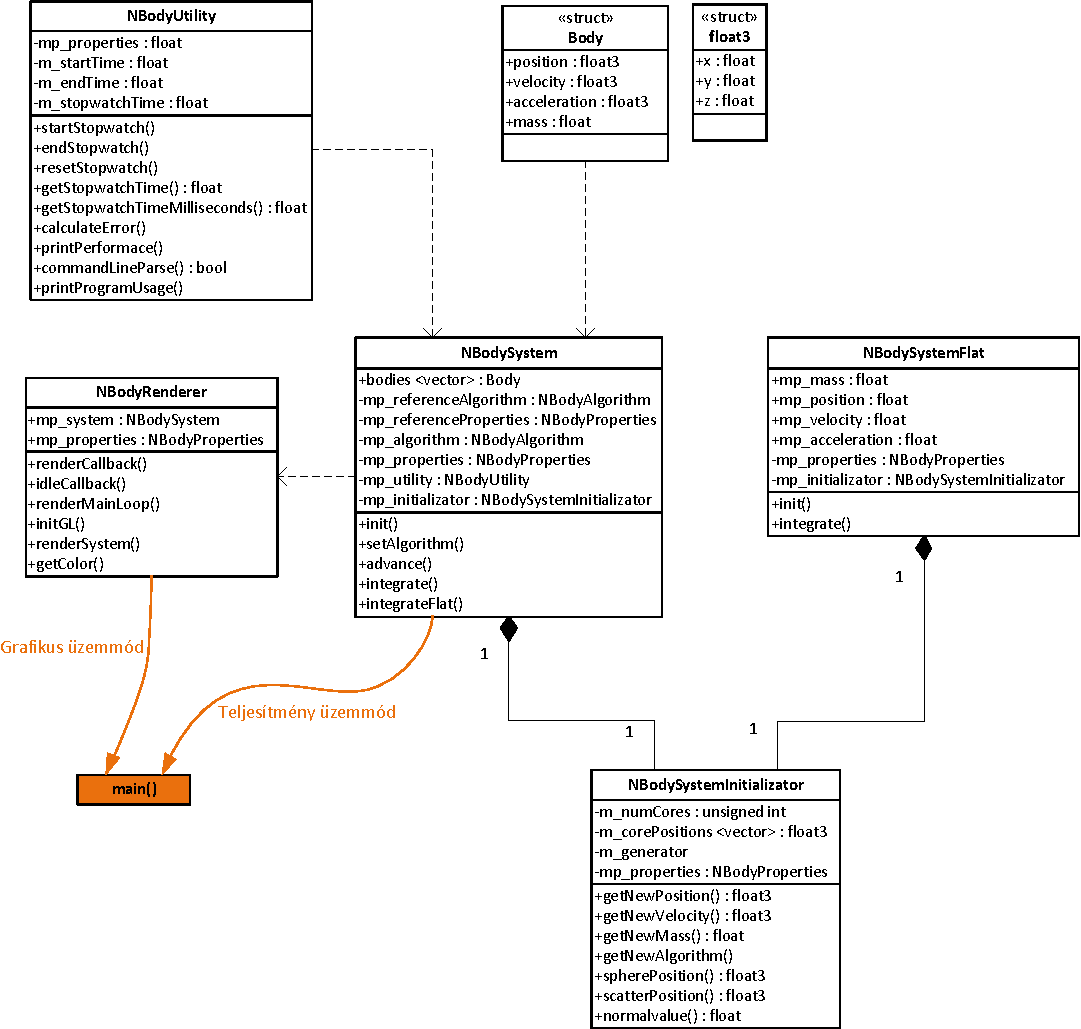
\includegraphics[width=150mm, keepaspectratio]{figures/Implementation/Impl_System-cropped.pdf}
		\caption{ A szimul�tor k�zponti oszt�lyai}
		\label{fig:Impl_System}
		\end{figure}

		%----------------------------------------------------------------------------
		\subsubsection{Body}
		%----------------------------------------------------------------------------
			Kont�nerstrukt�ra a testek tulajdons�gainak t�rol�s�ra. El�sz�r a mem�ri�ban val� adatt�rol�s szempontj�b�l kedvez�bb megold�st szerettem volna alkalmazni: elhelyezni a k�l�nb�z� testek azonos jelleg� tulajdons�gait egyszer� t�mb�kben (SoA - \emph{Structure of Arrays}). A jobb kezelhet�s�g �s �tl�that�s�g �rdek�ben, azonban logikailag sz�tv�lasztott strukt�ra mellett d�nt�ttem (AoS - \emph{Array of Structures}).

			Tartalmazza a test t�meg�t, aktu�lis poz�ci�-, sebess�g- �s gyorsul�svektor�t.

		%----------------------------------------------------------------------------
		\subsubsection{NBodySystem}
		%----------------------------------------------------------------------------
			A testeket t�rol� vektoron k�v�l sz�mos pointerrel rendelkezik a program t�bbi r�sz�re. Az \verb+init+ met�dus megh�v�s�val ker�lnek legener�l�sra a testek kezdeti param�terei, �gyelve arra, hogy k�t test ne legyen ,,t�l k�zel'' egym�shoz. Ennek akkor lenne jelent�s�ge, ha nem haszn�ln�nk a $\varepsilon$ t�nyez�t (l�sd \eqref{NBody_accEq} k�plet), ami numerikus szingularit�st hivatott megel�zni.
		
			A \verb+setAlgorithm+ a futtat�si konfigur�ci�ban (\verb+mp_properties+) be�ll�tottak alapj�n kiv�lasztja �s p�ld�nyos�tja a megfelel� algoritmust.
		
			Az \verb+advance+ tagf�ggv�ny h�vja meg az algoritmusban megval�s�tott, megegyez� nev� \verb+advance+ tagf�ggv�nyt. Ezt k�vet�en l�pteti az jelenlegi id�t, a megadott szimul�ci�s l�p�sk�zzel.
			
			Az \verb+integrate+ met�dus megh�v�s�val indul el a szimul�ci� (l�nyeg�ben egy ciklus, melynek a le�ll�si felt�tele, hogy a jelenleg eltelt id� nagyobb egyenl�, mint a le�ll�si id�).
		
			Az \verb+integrateFlat+ egy pr�b�lkoz�s volt a teljes�tm�ny jav�t�s�ra, a karbantarthat�bb oszt�lyhierarchia fel�ldoz�s�val. A f�ggv�nyh�v�sok rendszere �s az oszt�lyok megsz�ntet�s�vel egy ,,spagetti-k�d''-szer� f�ggv�ny. Err�l �s ennek eredm�ny�r�l a k�s�bbiekben m�g sz� lesz.
		
			Opcion�lisan p�ld�nyos�that� egy egy sz�lon fut� nat�v C++-os referencia algoritmus �s egy hozz�tartoz� \verb+NBodyProperties+. Ha be van kapcsolva ez az ellen�rz�s, akkor ennek is lefut az advance tagf�ggv�nye �s �sszehasonl�t�sra ker�lnek az eredm�nyek.

		%----------------------------------------------------------------------------
		\subsubsection{NBodySystemFlat}
		%----------------------------------------------------------------------------
			Szint�n egy pr�b�lkoz�s volt a teljes�tm�ny n�vel�s�re. A \verb+Body+ oszt�ly haszn�lata �s AoS megold�s helyett, egyszer�, dinamikusan allok�lt t�mb�ket hoztam l�tre. L�that�, hogy nem tartalmaz referenci�t semmilyen algoritmusra, ugyanis az \verb+integrate+ f�ggv�nyben val�s�tottam meg a sz�m�t�sokat. A teljes�tm�nyn�veked�s sz�mottev� volt, melyr�l majd a k�s�bbiekben besz�molok.
		
			Ez az oszt�ly csak a programk�d m�dos�t�s�val p�ld�nyos�that� �s haszn�lhat�, a felhaszn�l� �ltal nem.

		%----------------------------------------------------------------------------
		\subsubsection{NBodyInitializator}
		%----------------------------------------------------------------------------
			Feladata a testek kezdeti attrib�tumait felt�lteni v�letlenszer�en gener�lt, norm�lis eloszl�s� �rt�kekkel. A testeket az \verb+NBodyProperties+ \verb+formation+ mez�j�ben be�ll�tott �rt�k alapj�n helyezi el. Lehetnek az orig� k�r�l sz�tsz�rtan vagy v�letlenszer�en l�trehozott pontok k�rny�k�n, nagyj�b�l egyenletesen sz�tosztva.
		
			A megfelel� algoritmust is ez az oszt�ly p�ld�nyos�tja �s inicializ�lja.

		%----------------------------------------------------------------------------
		\subsubsection{NBodyRenderer}
		%----------------------------------------------------------------------------
			Az oszt�ly teljesen statikus, p�ld�ny nem hozhat� l�tre. Erre a \emph{callback} f�ggv�nyek haszn�lata miatt volt sz�ks�g, melyeket az OpenGL haszn�l, miut�n megh�v�dott a vez�rl� ciklus�t tartalmaz� f�ggv�nye. 
		
			Az \verb+initGL+ tagf�ggv�ny �ll�tja be a legfontosabb parem�tereket, pl.: ablak m�ret, h�tt�rsz�n, �lsim�t�s.
		
			A \verb+renderCallback+ az, ami megh�vja a p�ld�nyos�tott \verb+NBodySystem+ \verb+advance+ met�dus�t �s m�ri az eltelt szimul�ci�s id�t. Miut�n kisz�m�t�sra ker�ltek az �j poz�ci��rt�kek, megh�vja a \verb+renderSystem+ nev� f�ggv�nyt, mely kirajzoltatja az egyes pontokat a k�perny�re. Ez haszn�lja fel a \verb+getColor+ nev� seg�df�ggv�nyt, mely minden testnek be�ll�tja a sz�n�t, a k�zel�ben elhelyezked� testek sz�ma alapj�n. Min�l t�bb ,,szomsz�dja'' van ann�l vil�gosabb a sz�ne.
		
			A \verb+main+ f�ggv�ny az, amely ennek az oszt�lynak a tagf�ggv�nyeit felhaszn�lja. Grafikus kijelz�sn�l nincs id�- �s teljes�tm�nym�r�s.

		%----------------------------------------------------------------------------
		\subsubsection{NBodyUtility}
		%----------------------------------------------------------------------------
			Kieg�sz�t�, seg�doszt�ly szerepet t�lt be. Feladatai a felhaszn�l� be�ll�t�sok �rtelmez�se (\verb+commandLineParse+ f�ggv�ny), az id�- �s teljes�tm�nym�r�s, valamint a hibasz�m�t�s.
		
			A program a fel�ll�s ut�n a \verb+*Stopwatch+ kifejez�st tartalmaz� f�ggv�nyek seg�ts�g�vel m�ri le a szimul�ci� hossz�t. Kisz�molja, hogy �sszesen h�ny er�t kellett kisz�molni, h�ny lebeg�pontos oper�ci�t v�gzett el �sszesen a program �s ezek f�ggv�ny�ben �rja ki a fut�si teljes�tm�nyt.
		
			Amennyiben~~~referenciamodellt~~~haszn�lunk,~~minden~~iter�ci�~~ut�n~~megh�v�dik~~a~~\verb+calculateError+ met�dus, ami minden testnek �sszehasonl�tja a poz�ci�j�t �s jelzi azonnal, ha l�nyeges �rt�kbeli elt�r�st tapasztalt.

		%----------------------------------------------------------------------------
		\subsubsection{A main f�ggv�ny}
		%----------------------------------------------------------------------------
			Itt ker�l p�ld�nyos�t�sra minden k�zponti oszt�ly, melyek azt�n \verb+shared pointer+-rel hivatkoznak egym�sra.
		
			Ha grafikus kijelz�s be lett �ll�tva, akkor az \verb+NBodyRenderer+ \verb+renderMainLoop+ statikus tagf�ggv�nye veszi �t a vez�rl�st. Teljes�tm�nym�r�s �zemm�d eset�n pedig az \verb+NBodySystem+ \verb+integrate+ met�dusa v�gzi a szimul�ci�t.

			A \figref{Impl_ProgramInitSeq} �s a \figref{Impl_SimulationSeq} �bra a szimul�tor m�k�d�s�t mutatja be. Az egyes f�zisok egym�st k�vetik, de k�l�n-k�l�n jobban �br�zolhat�k.

			\begin{figure}[!ht]
			\centering
			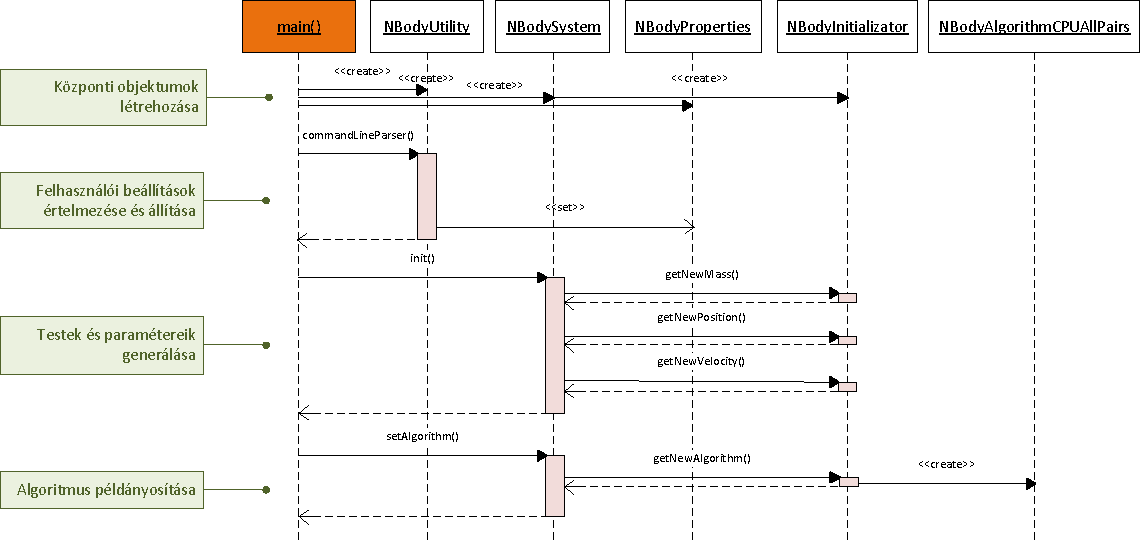
\includegraphics[width=150mm, keepaspectratio]{figures/Implementation/Impl_ProgramInitSeq-cropped.pdf}
			\caption{A program inicializ�ci�s f�zisa}
			\label{fig:Impl_ProgramInitSeq}
			\end{figure}
			
			\begin{figure}[!ht]
			\centering
			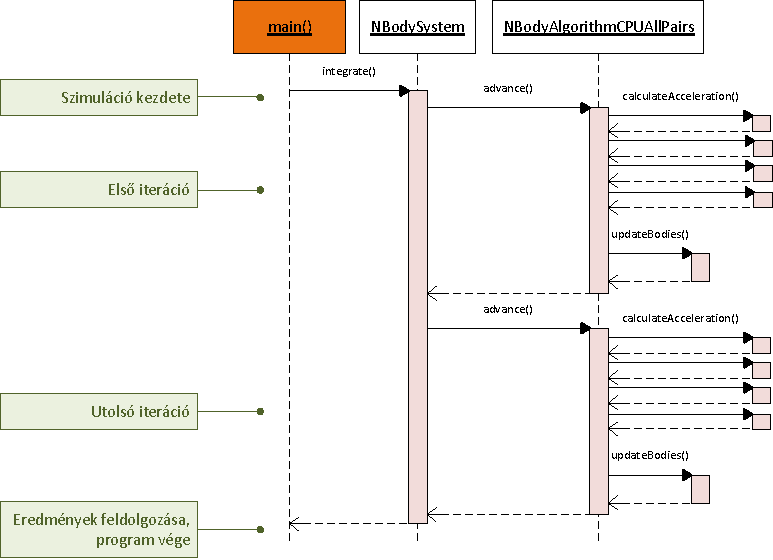
\includegraphics[width=150mm, keepaspectratio]{figures/Implementation/Impl_SimulationSeq-cropped.pdf}
			\caption{A program szimul�ci�s f�zisa}
			\label{fig:Impl_SimulationSeq}
			\end{figure}

	
	%----------------------------------------------------------------------------
\section{C++ referencia modell}
%----------------------------------------------------------------------------
	Az egy sz�lon fut� C++ referenciamodell megval�s�t�st a MATLAB-ban meg�rt verzi� alapj�n kezdtem el. C�lja, hogy viszony�t�si alapk�nt szolg�ljon a k�l�nb�z� p�rhuzamos�t�st alkalmaz� implement�ci�khoz, ezzel lehet�v� t�ve a sz�mszer�/grafikus �br�zol�s�t a sebess�gn�veked�snek.

	A p�rhuzamos�t�st a CPU-n f�k�nt a legbels�, gyorsul�s �rt�keket kisz�m�t� \verb+calculateAcceleration+ f�ggv�ny m�dos�t�s�val �rtem el. A megval�s�tott k�plet mindig az \sectref{NBody_integrateSect} fejezetben bemutatott \eqref{NBody_accEq} �sszef�gg�s.

	Az al�bbi k�dr�szlet a teljesen nat�v C++ megval�s�t�s:
	
	\begin{lstlisting}
float3 NBodyAlgorithmCPU::calculateAcceleration(
const float3 posI, 	 // A test, melynek a gyorsul�s �rt�k�nek egy darabj�t sz�moljuk
const float massJ, 	 // A m�sik test t�mege
const float3 posJ) { // A m�sik test poz�ci�ja
   
	float3 r, accI;

	// A k�t test t�vols�gvektora
	r.x = posJ.x - posI.x;
	r.y = posJ.y - posI.y;
	r.z = posJ.z - posI.z;

	// A k�t test skal�ris t�vols�ga belekalkul�lva az �n. softening factor-t
	float rabs = sqrt(r.x * r.x + r.y * r.y + r.z * r.z + mp_properties->EPS2);
	// A k�pletben megadott nevez� kisz��t�sa
	float rabsInv = 1.0f / (rabs * rabs * rabs);

	// A j. test t�meg�be bele van olvasztva a G �rt�ke,
	// hogy ne kelljen mindig �sszeszorozni.
	float temp = massJ * rabsInv;

	// A k�plet m�sodik tagja.
	// Az i. testen a j. test �ltal okozott gyorsul�s
	accI.x = r.x * temp;
	accI.y = r.y * temp;
	accI.z = r.z * temp;

	return accI;
}
	\end{lstlisting}
	
	�sszesen 17 egyszeres pontoss�g� lebeg�pontos m�veletet (FLOP - Floating Point Operation) hajt v�gre, egy testp�r k�z�tti gyorsul�s kisz�m�t�s�hoz �s m�g 3 �sszead�st a f�ggv�nyen k�v�l, az akkumul�l�shoz. Ezt a f�ggv�nyt kell $N^2$-szer megh�vni minden testp�rra, ahol $N$ a testek sz�ma.

	Az al�bbi k�dr�szleteket az egyik els� verzi�b�l val� azok k�z�l, amit �rtam. A t�bbi egy kicsit jobban feldarabolt a p�rhuzamos�t�s miatt. Viszont az alapelv v�ltozatlan �s ebben a form�ban k�nnyebben �rtelmezhet�.

	A testeket egy \verb+vector+ kont�nerben t�rolom, ami a dinamikus t�mbkezel�s probl�m�it (allok�ci�, reallok�ci�, felszabad�t�s) neh�zs�geit veszi le a fejleszt�k v�ll�r�l.

	A \verb+bodies vector+$ i.$ elem�t, vagyis az i. testet, valamint annak a gyorsul�s�t az al�bbiak szerint �rj�k el:
	
	\begin{lstlisting}
bodies						// a testeket tartalmaz� vector
bodies.at(i)				// az i. test (Body strukt�r�val t�r vissza)
bodies.at(i).acceleration   // az i. test gyorsul�svektora (float3)
bodies.at(i).acceleration.x // az i. test x ir�ny� gyorsul�s �rt�ke (float)
	\end{lstlisting}

	A m�r eml�tett \verb+advance+ f�ggv�ny belsej�ben tal�lhat� kett�, egym�sba �gyazott for ciklus. A k�ls� ciklus mindig az �ppen gyorsul�s szempontj�b�l friss�tend� testet jel�li ki, m�g a bels� a p�rj�t. A ciklusmag mindig az el�z� szimul�ci�s iter�ci�ban kisz�molt gyorsul�s �rt�kek kinull�z�s�val kezd�dik.

	\begin{lstlisting}
void NBodyAlgorithmCPUAllPairs::advance(std::vector<Body> &bodies) {
	...
	for (int i = 0; i < mp_properties->numBody; i++) {
		// Az el�z� iter�ci�ban kisz�molt gyorsul�svektor kinull�z�sa
		float3 zeros = float3(0.0f, 0.0f, 0.0f);
		
		bodies.at(i).acceleration = zeros;

		float3 acc = zeros;
		for (int j = 0; j < mp_properties->numBody; j++) {
			// 17 FLOP
			acc = calculateAcceleration(bodies.at(i).position, bodies.at(j).mass, bodies.at(j).position);
			// 3 FLOP
			bodies.at(i).acceleration.x += acc.x;
			bodies.at(i).acceleration.y += acc.y;
			bodies.at(i).acceleration.z += acc.z;
		}
	}
	...
}
	\end{lstlisting}
	
	Annak �rdek�ben, hogy az egyes gyorsul�s �rt�kek, konzisztens poz�ci�adatokb�l legyen kisz�m�tva, az integr�l�s (\eqref{NBody_integrateEq} k�plet) v�grehajt�s�t egy m�sik ciklusban kell elv�gezni. �sszesen $N$-szer v�grehajtani a ciklust, iter�ci�nk�nt ez 21 FLOP-ot jelent. Ebb�l 3 FLOP-ot, hoz be egy gyorsul�s �rt�k�t cs�kkent� plusz konstans, melynek feladata, hogy a szimul�ci� sor�n ne hagyja a testeket egym�st�l nagyon elt�volodni. A grafikus megjelen�t�s r�gz�tett, nem mozd�that� vagy forgathat� �s gyakran j�nnek, mennek az ablak sz�l�n a testek.

	\begin{lstlisting}
float stepTime2 = 0.5f * mp_properties->stepTime * mp_properties->stepTime;

for (int i = 0; i < mp_properties->numBody; i++) {
	// Poz�ci�vektor friss�t�se
	// 3*4 FLOP
	bodies.at(i).position.x += bodies.at(i).velocity.x * mp_properties->stepTime +
		bodies.at(i).acceleration.x * stepTime2;
	bodies.at(i).position.y += bodies.at(i).velocity.y * mp_properties->stepTime +
		bodies.at(i).acceleration.y * stepTime2;
	bodies.at(i).position.z += bodies.at(i).velocity.z * mp_properties->stepTime +
		bodies.at(i).acceleration.z * stepTime2;

	// Sebess�gvektor friss�t�se
	//3*3 FLOP
	bodies.at(i).velocity.x = bodies.at(i).velocity.x * mp_properties->VELOCITY_DAMPENING +
		bodies.at(i).acceleration.x * mp_properties->stepTime;
	bodies.at(i).velocity.y = bodies.at(i).velocity.y * mp_properties->VELOCITY_DAMPENING +
		bodies.at(i).acceleration.y * mp_properties->stepTime;
	bodies.at(i).velocity.z = bodies.at(i).velocity.z * mp_properties->VELOCITY_DAMPENING +
		bodies.at(i).acceleration.z * mp_properties->stepTime;
}
	\end{lstlisting}

	
	%----------------------------------------------------------------------------
\section{OpenMP}
%----------------------------------------------------------------------------
	Els� l�p�sben az egyik legegyszer�bben el�rhet� �s relat�ve kev�s munk�t ig�nyl� OpenMP felhaszn�l�s�val igyekeztem a munk�t sz�tosztani sz�lak k�z�tt. Kiv�l�an alkalmazhat� olyan probl�m�k eset�n, ahol a p�rhuzamos�tand� r�szek m�rete fut�si id�ben d�l el.

	Az OpenMP (Open Multi-Processing) egy specifik�ci�, a kieg�sz�t�se a C �s C++ nyelveknek, mely m�r igen sz�lesk�r� t�mogatotts�got �lvez a nagy hardver- �s szoftvergy�rt�k r�sz�r�l. 

	A kieg�sz�t�s els�sorban ford�t� direkt�v�kat defini�l, melyek haszn�lat�val kijel�lhet�k a k�dban azok a program r�szek, amelyeket szeretn�nk, ha a ford�t� megpr�b�lna p�rhuzamos�tani. Az �gynevezett \emph{fork-join} modellt val�s�tja meg az OpenMP, melyben a teljes program feloszthat� egym�st k�vet� szekvenci�lis �s p�rhuzamos r�szekre. A program sorosan v�grehajtand� k�ddal indul, majd el�gazik egym�st�l f�ggetlen r�szekre �s v�g�l �jra egyes�l \cite{omp}.

	\begin{figure}[!ht]
	\centering
	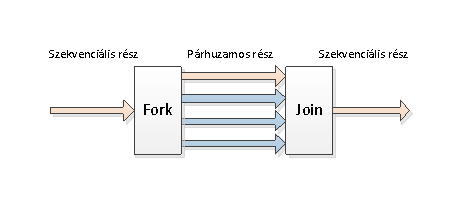
\includegraphics[width=150mm, keepaspectratio]{figures/Implementation/Impl_OMP_ForkJoin.pdf}
	\caption{Fork-join modell}
	\label{fig:Impl_ForkJoin}
	\end{figure}

	Bizonyos helyzetekben el�g n�h�ny sort be�rni egy teljesen szekvenci�lis programba �s m�ris sz�mottev� n�veked�st lehet el�rni. Mind minden p�rhuzamos�t�si technol�gi�n�l itt is figyelni kell a k�z�s haszn�lat� v�ltoz�kra, amennyiben van ilyen. Bizonyos ford�t�k automatikusan sz�tosztj�k a feladatokat a processzormagok k�z�tt.

	Az egyik legjobban p�rhuzamos�that� programr�sz, az egym�st�l \emph{f�ggetlen adatokkal dolgoz� ciklus}. A megold�s itt az jelenti, ha a ciklust feldaraboljuk, annyi kisebb ciklusra ah�ny sz�lat szeretn�nk l�trehozni. A keletkezett kisebb ciklusok v�grehajt�s�t pedig sz�tosztjuk a magok k�z�tt:

	\begin{lstlisting}
// Eredeti ciklus
for(int i = 0; i < N ; i++) {
	c[i] = a[i] + b[i];
}

// 4 ciklusra felbontva
for(int i = 0; i < N/4 ; i++) {...}		 // 1. mag
for(int i = N/4; i < N/2 ; i++) {...}   // 2. mag
for(int i = N/2; i < 3*N/4 ; i++) {...} // 3. mag
for(int i = 3*N/4; i < N ; i++) {...}   // 4. mag
	\end{lstlisting}

	A magok k�z�tti sz�toszt�st a fenti m�dszerrel m�g nem tett�k meg, viszont �gy l�that�, hogy milyen ir�nyb�l k�zel�ti meg a probl�m�t az OpenMP. Az al�bbi \verb+pragma+ direkt�v�val kieg�sz�tett k�d hat�s�ra a ford�t� p�rhuzamos�tani fogja a k�zvetlen�l ut�na k�vetkez� \verb+for+ ciklust. Minden sz�lhoz l�trehoz egy ciklusv�ltoz�t lok�lisan, a t�bbi kor�bban deklar�lt v�ltoz� $(N, a, b, c)$ viszont k�z�s haszn�lat�. a \verb+num_threads(x)+ hat�rozza meg a l�trehozand� sz�lak sz�m�t. Amennyiben nincs megadva az alap�rtelmezett �rt�k a maximum el�rhet� sz�lsz�m lesz. Esetemben ez az \tabref{szgspecifikacio} t�bl�zat alapj�n 8.

	\begin{lstlisting}
#pragma omp parallel for num_threads(4)
for(int i = 0; i < N ; i++) {
	c[i] = a[i] + b[i];
}
	\end{lstlisting}
	
	A referencia algoritmusban bemutatott k�t \verb+for+ ciklus k�z�l a k�ls�t �rdemes p�rhuzamos�tani. Ezzel minden mag k�l�nb�z� testnek fogja a gyorsul�s �rt�keit friss�teni, s nem lesz sz�ks�ges semmif�le szinkroniz�ci� vagy atomi m�velet haszn�lata. A ciklusv�ltoz� �s a gyorsul�s�rt�kek ideiglenes t�rol�s�ra l�trehozott bel�l lett deklar�lva, �gy minden sz�l sz�m�ra lok�lis v�ltoz�k lesznek.

	Mivel ford�t�sidej� p�rhuzamos�t�sr�l van sz�, annak megold�s�t, hogy ez a funkci� ki-bekapcsolhat� legyen, n�mi redundancia seg�ts�g�vel �rtem el:
	
	\begin{lstlisting}
void NBodyAlgorithmCPUAllPairs::advance(std::vector<Body> &bodies) {
	...
	if (mp_properties->useOpenMP) {
	#pragma omp parallel for
		for (int i = 0; i < mp_properties->numBody; i++) {
			// Bels� for ciklus, �s a calculateAcceleration() met�dus h�v�sa
		}
	}
	else {
		for (int i = 0; i < mp_properties->numBody; i++) {
			// Bels� for ciklus, �s a calculateAcceleration() met�dus h�v�sa
		}
	}
	...
}
	\end{lstlisting}

	A k�t \verb+for+ ciklus k�z�l csak az egyik el� ker�lt \verb+pragma+ direkt�va, a m�sik teljesen szekvenci�lis maradt. A ford�t�s ut�n a \verb+boolean+ t�pus� \verb+useOpenMP+ v�ltoz� �ll�t�s�val lehet v�lasztani k�z�l�k. Hasonl� megold�ssal az integr�l� r�sz \verb+for+ ciklus�t is p�rhuzamos�tottam.

	Egy m�sik remek OpenMP direkt�va, a szint�n ciklusok el� �rhat� az \verb+unroll+. Ezt akkor �rdemes haszn�lni, ha egy ciklusnak a magja kev�s utas�t�sb�l �ll, vagyis a felt�telvizsg�lat �s a hozz�tartoz� ugr� utas�t�s sz�mottev�, �sszem�rhet� r�szt tesz ki a ,,hasznos'' k�ddal. Ennek hat�s�ra a ciklus mag t�bbsz�r egym�s al� m�sol�dik a mem�ri�ban, �s a ciklusv�ltoz� nagyobb l�pt�k� lesz.

	\begin{lstlisting}
#pragma unroll(4)
for(int i = 0; i < N ; i++) {
	c[i] = a[i] + b[i];
}
	\end{lstlisting}

	A fenti k�d hat�sa ekvivalens lesz:

	\begin{lstlisting}
for(int i = 0; i < N ; i += 4) {
	c[i]   = a[i]   + b[i];
	c[i+1] = a[i+1] + b[i+1];
	c[i+2] = a[i+2] + b[i+2];
	c[i+3] = a[i+3] + b[i+3];
}
	\end{lstlisting}

	Ezzel a vez�rl� (control-flow) utas�t�sok ar�nya cs�kkent, a ciklus mag utas�t�sainak sz�m�hoz k�pest. A ford�t�k sokszor automatikusan �lnek ezzel a megold�ssal. Ha N kicsi el�fordulhat, hogy a ciklus teljes m�rt�kben ki lesz bontva. Egyetlen h�tr�nya az \verb+unroll+-nak, hogy a k�d hosszabb lesz �s t�bb helyet foglal ford�t�s ut�n.

	L�that�, hogy a szimul�tor sz�m�t�sig�nyesebb r�szeit mind�sszesen k�t sor be�r�s�val siker�lt p�rhuzamos�tani, a probl�ma jelleg�b�l ad�d�an. A f�ggetlen sz�m�t�sokat tartalmaz� k�dr�szletek, nagyon hat�konyan p�rhuzamos�that�k OpenMP seg�ts�g�vel. A profilert eredm�nye l�that� a \figref{Impl_basic_vs_omp} �br�n, a n�gy magos CPU kihaszn�lts�ga jelent�sen megn�vekedett �s a fut�si id� ler�vid�lt.

	\begin{figure}[!ht]
	\centering
	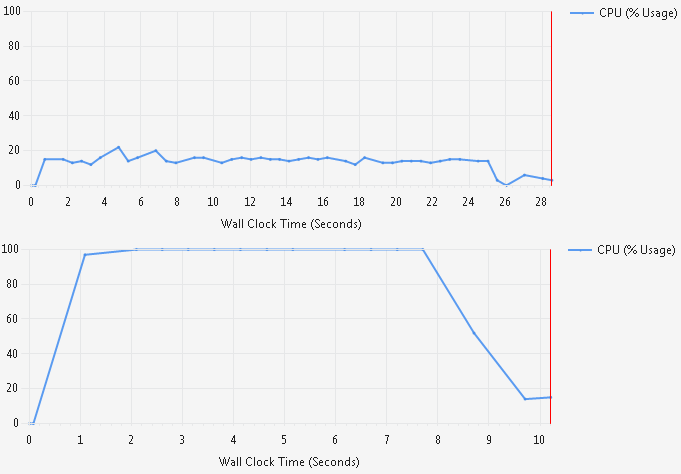
\includegraphics[width=150mm, keepaspectratio]{figures/Performance/basic_vs_omp.png}
	\caption{$1024$ test, $1000$ iter�ci� szimul�ci� fut�si eredm�nye OpenMP n�lk�l �s OpenMP-vel}
	\label{fig:Impl_basic_vs_omp}
	\end{figure}

	Az OpenMP haszn�lat�nak m�sik el�nye, hogy a soron k�vetkez� SSE �s AVX megold�sokkal egy�tt haszn�lhat�, ugyanis el�bbi a processzormagok k�z�tti, a m�sik kett� pedig magokon bel�li p�rhuzamos�t�s.

	
	%----------------------------------------------------------------------------
\section{SSE}
%----------------------------------------------------------------------------
	A k�vetkez� CPU-s p�rhuzamos�t�si lehet�s�g m�r megk�vetelte a legbels�, gyorsul�st sz�m�t� f�ggv�ny m�dos�t�s�t.

	Az Intel SSE (Streaming SIMD Extensions) egy utas�t�sk�szlet kieg�sz�t�s, mely be�p�tett speci�lis 128 bit sz�les vektorregiszterekkel dolgozik. A neve is tartalmazza az �ltala megval�s�tott SIMD (Single Instruction Multiple Data) modellt. Kor�bbi fejezetben eml�t�sre ker�lt, hogy ez egyben egy csoportos�t�s, a Flynn f�le taxon�mia r�sze. L�nyege, hogy egyszerre \emph{t�bb, azonos t�pus� adaton} egyszerre v�grehajt�dik ugyanaz az \emph{egy darab utas�t�s}, ezzel adatszint� p�rhuzamos�t�st val�s�tva meg. El�nye az egyszer� (SISD) sz�m�t�g�pekkel szemben egy�rtelm�en a kevesebb utas�t�s-felhozatal, vagyis kevesebb mem�riam�velet, ami gyakori korl�t p�rhuzamos programok �r�sa eset�n.

	SSE eset�ben bet�lthet� a 128 bites regiszterbe 4 darab egyszeres pontoss�g� lebeg�pontos sz�m, melyen v�grehajthat�k a vektorutas�t�sok. Az \figref{Impl_SIMD} �br�n egy SIMD p�lda l�that�: SSE regisztereken v�gzett �sszead�s.

	\begin{figure}[!ht]
	\centering
	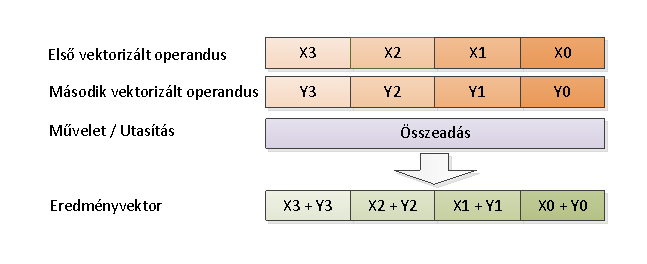
\includegraphics[width=150mm, keepaspectratio]{figures/Implementation/Impl_SSE_SIMD.pdf}
	\caption{SIMD modell}
	\label{fig:Impl_SIMD}
	\end{figure}

	Ahhoz, hogy ne kelljen x86 ASM programot �rni a ford�t�k biztos�tanak �gynevezett \emph{intrinsic header} f�jlokat, melyek elfedik, �s k�zvetlen�l haszn�lhat�v� teszik az SSE utas�t�sokat \cite{sse}.

	A kor�bbiakban haszn�lt t�mbelemek �sszead�s maradva:
	
	\begin{lstlisting}
for(int i = 0; i < N; i += 4) {
	// Operandusok bet�lt�se
	__m128 av =  _mm_set_ps(a[i+3], a[i+2], a[i+1], a[i]);
	__m128 bv =  _mm_set_ps(b[i+3], b[i+2], b[i+1], b[i]);

	// Egy �sszed�s m�velet elv�gz�se a k�t v�ltoz�n
	__m128 cv =  _mm_add_ps(av, bv);

	// Eredm�nyek bet�lt�se a c t�mbbe
	_mm_strore_ps(&c[i], cv);
}
	\end{lstlisting}
	
	Itt az�rt l�nyeges v�ltoz�sokon esett �t a k�d. El�sz�r is l�that�, hogy kev�sb� olvashat� lett. Ez sajnos az SSE intrinsic haszn�lat�nak egy rossz mell�khat�sa. Bet�lt (\verb+_mm_set_ps+) n�gy egym�st k�vet� �s egym�st�l f�ggetlen (\verb+float+) v�ltoz�t \verb+a+, \verb+b+ t�mbb�l egy-egy 128 bites regiszterbe. A k�t regisztert ezut�n �sszeadja (\verb+_mm_add_ps+) �s az \figref{Impl_SIMD} �br�nak megfelel� eredm�nyvektort kapjuk. Ezt k�vet�en t�rt�nik a 4 elem m�sol�sa (\verb+_mm_strore_ps+) az eredm�nyt tartalmaz� \verb+c+ t�mbbe. Egy megk�t�s sajnos van. A \verb+c+ t�mb�t �gy kell deklar�lni, hogy az egy $128$-cal oszthat� kezd�c�mre mutasson, m�sk�l�nben fut�si idej� hib�t kapunk (access violation). Ez az SSE egy saj�toss�ga, amennyiben az egyik argumentum a rendszermem�ri�ban helyezkedik el.

	\begin{lstlisting}
float *c = (float *)(_aligned_malloc(N * sizeof(float), 16));
...
_aligned_free(c);
	\end{lstlisting}
	
	M�sik elt�r�s is l�that� a \verb+for+ ciklus param�terei k�z�tt. A ciklus v�ltoz� n�ggyel n�vekedik, ugyanis egy iter�ci� sor�n egyszerre 4 elem feldolgoz�sa t�rt�nik. Jelen p�ld�ban egy \verb+N%4 == 0+ megk�t�ssel �rdemes �lni.

	�t�ltetve az eddigiekben elmondottak az intrinsic-et haszn�l� \verb+calculateAcceleration+ met�dus az al�bbiak szerint alakul:

	\begin{lstlisting}
void NBodyAlgorithmCPU::calculateAcceleration(const float3(&posI)[4],
	const float massJ, const float3 posJ, float *accI) {

	// A k�t test poz�ci�vektor�nak bet�lt�se, k�l�n szedve az x, y �s z koordin�t�kat
	__m128 pix = _mm_set_ps(posI[3].x, posI[2].x, posI[1].x, posI[0].x);
	__m128 piy = _mm_set_ps(posI[3].y, posI[2].y, posI[1].y, posI[0].y);
	__m128 piz = _mm_set_ps(posI[3].z, posI[2].z, posI[1].z, posI[0].z);

	__m128 pjx = _mm_set_ps1(posJ.x);
	__m128 pjy = _mm_set_ps1(posJ.y);
	__m128 pjz = _mm_set_ps1(posJ.z);

	// T�vols�gvektorok kisz�m�t�sa
	__m128 rx = _mm_sub_ps(pjx, pix);
	__m128 ry = _mm_sub_ps(pjy, piy);
	__m128 rz = _mm_sub_ps(pjz, piz);

	__m128 eps2 = _mm_set_ps1(mp_properties->EPS2);

	// T�vols�gvektorok hossz�nak sz�m�t�sa
	__m128 rx2 = _mm_mul_ps(rx, rx);
	__m128 ry2 = _mm_mul_ps(ry, ry);
	__m128 rz2 = _mm_mul_ps(rz, rz);
	__m128 rabs = _mm_sqrt_ps(_mm_add_ps(_mm_add_ps(rx2, ry2), _mm_add_ps(rz2, eps2)));

	// K�plet nevez�j�nek meghat�roz�sa
	__m128 m = _mm_set_ps1(massJ);
	__m128 rabsInv = _mm_div_ps(m, _mm_mul_ps(_mm_mul_ps(rabs, rabs),rabs));

	// Gyorsul�s�rt�kek kisz�m�t�sa
	__m128 aix = _mm_mul_ps(rx, rabsInv);
	__m128 aiy = _mm_mul_ps(ry, rabsInv);
	__m128 aiz = _mm_mul_ps(rz, rabsInv);

	// Gyorsul�s�rt�k�kek visszam�sol�sa a megadott float t�mbbe (x,x,x,x,y,y,y,y,z,z,z,z) form�ban
	_mm_store_ps(accI, aix);
	_mm_store_ps(accI + 4, aiy);
	_mm_store_ps(accI + 8, aiz);
}
	\end{lstlisting}
	
	A f�ggv�ny elej�n t�rt�nik a v�ltoz�k bet�lt�se az \verb+_mm_set_ps+ �s az \verb+_mm_set_ps1+ f�ggv�nyek seg�ts�g�vel. Ez ut�bbi mind a n�gy ,,rekeszt'' felt�lti a megadott \verb+float+ �rt�kkel. A vektor v�ltoz�kkal ezut�n ugyan�gy a sz�m�t�sok k�vetkeznek, mint az �sszead�s p�ld�ban, majd az eredm�nyek visszam�sol�sa a rendszermem�ri�ba. Az kisz�molt gyorsul�s�rt�kek akkumul�l�s�n�l figyelembe kell venni, hogy a t�mb elej�n az $x$, k�zep�n az $y$ �s a v�g�n a $z$ koordin�t�k szerepelnek.

	Ak�r csak a p�ld�ban a \verb+for+ ciklust is m�dos�tottam:

	\begin{lstlisting}
...
// 128-cal oszthat� kezd�c�m� t�mb allok�l�sa
float *accI = (float *)(_aligned_malloc(12 * sizeof(float), 16));

for (int i = 0; i < mp_properties->numBody; i += 4) {
	for (int j = 0; j < mp_properties->numBody; j++) {
       
		calculateAcceleration(bodies.at(i).position, bodies.at(j).mass, bodies.at(j).position, accI);

		// Akkumul�l�s
		bodies.at(i).acceleration.x += accI[0];
		bodies.at(i).acceleration.y += accI[4];
		bodies.at(i).acceleration.z += accI[8];
		bodies.at(i + 1).acceleration.x += accI[1];
		bodies.at(i + 1).acceleration.y += accI[5];
		bodies.at(i + 1).acceleration.z += accI[9];
		bodies.at(i + 2).acceleration.x += accI[2];
		bodies.at(i + 2).acceleration.y += accI[6];
		bodies.at(i + 2).acceleration.z += accI[10];
		bodies.at(i + 3).acceleration.x += accI[3];
		bodies.at(i + 3).acceleration.y += accI[7];
		bodies.at(i + 3).acceleration.z += accI[11];
	}
}
_aligned_free(accI);
...
	\end{lstlisting}
	
	A kisz�molt gyorsul�s�rt�keket tartalmaz� t�mb�t a 128-cal oszthat� c�mre allok�ltam, mert az lesz a \verb+_mm_store_ps+ utas�t�s c�lpontja. Az akkumul�l�st r�sz direkt van teljesen kibontva. Ciklussal is le lehet ugyan �rni, ami szebb, de az a megold�s lassabb lesz. OpenMP \verb+unroll+ direkt�v�s megold�s egy kicsivel volt csak rosszabb enn�l. Tekintve, hogy az akkumul�l�st v�gz� \verb+for+ ciklus $N \cdot N/4$-szer futna le, nagy $N$ eset�re sok control-flow jelleg� utas�t�st jelent.

	Az integr�l�st v�gz� k�dr�szletet nem m�dos�tottam SSE f�ggv�nyekkel, ugyanis ,,nagy'' $N$ mellett a nyert sebess�gn�veked�s eleny�sz�, tekintve, hogy testsz�mmal line�ris a komplexit�sa.

	Az SSE intrinsic f�ggv�nyek haszn�lat�nak nagy probl�m�ja, hogy a k�d sokkal nehezebben olvashat� �s ellen�rizhet�. H�tr�nya m�g, hogy nem minden algoritmus vektoriz�lhat� egyszer�en, valamint az automatikus, ford�t� �ltali vektoriz�ci� legt�bbsz�r nem ad optim�lis megold�st; gyakran hardverk�zeli programoz�s sz�ks�ges a megfelel� teljes�tm�ny el�r�s�hez. Ezt C/C++ k�dba �gyazott SSE ASM bet�tek (k�dblokkok) haszn�lat�val tehetj�k meg.

	
	%----------------------------------------------------------------------------
\section{AVX}\label{sect:Impl_AVXSect}
%----------------------------------------------------------------------------
	Az AVX (Advanced Vector eXtension) az SSE-hez hasonl� SIMD jelleg� utas�t�sk�szlet kieg�sz�t�s. 2011-ben jelent az Intel Sandy Bridge mikroarchitekt�r�j�val. A felhaszn�lt regiszterek itt m�r 256 bit sz�lesek, vagyis egyszerre ak�r 8 \verb+float+ t�pus� adat is kezelhet� vele p�rhuzamosan. Ezekhez is van ford�t�kba be�p�tett intrinsic header, vagyis programoz�sa elm�letben nem okoz k�l�n�sebb neh�zs�get az SSE ut�n. A k�d ugyan�gy nehezen olvashat�.

	\begin{lstlisting}
void NBodyAlgorithmCPU::calculateAcceleration(const float3(&posI)[8],
	const float massJ, const float3 posJ, float *accI) {
	// A k�t test poz�ci�vektor�nak bet�lt�se, k�l�n szedve az x, y �s z koordin�t�kat
	__m256 pix = _mm256_set_ps(posI[7].x, posI[6].x, posI[5].x, posI[4].x, posI[3].x, posI[2].x, posI[1].x, posI[0].x);
	__m256 piy = _mm256_set_ps(posI[7].y, posI[6].y, posI[5].y, posI[4].y, posI[3].y, posI[2].y, posI[1].y, posI[0].y);
	__m256 piz = _mm256_set_ps(posI[7].z, posI[6].z, posI[5].z, posI[4].z, posI[3].z, posI[2].z, posI[1].z, posI[0].z);

	__m256 pjx = _mm256_set1_ps(posJ.x);
	__m256 pjy = _mm256_set1_ps(posJ.y);
	__m256 pjz = _mm256_set1_ps(posJ.z);
	
	// T�vols�gvektorok kisz�m�t�sa
	__m256 rx = _mm256_sub_ps(pjx, pix);
	__m256 ry = _mm256_sub_ps(pjy, piy);
	__m256 rz = _mm256_sub_ps(pjz, piz);
	
	__m256 eps2 = _mm256_set1_ps(mp_properties->EPS2);

	// T�vols�gvektorok hossz�nak sz�m�t�sa
	__m256 rx2 = _mm256_mul_ps(rx, rx);
	__m256 ry2 = _mm256_mul_ps(ry, ry);
	__m256 rz2 = _mm256_mul_ps(rz, rz);
	__m256 rabs = _mm256_sqrt_ps(_mm256_add_ps(_mm256_add_ps(rx2, ry2), _mm256_add_ps(rz2, eps2)));

	// K�plet nevez�j�nek meghat�roz�sa
	__m256 m = _mm256_set1_ps(massJ);
	__m256 rabsInv = _mm256_div_ps(m, _mm256_mul_ps(_mm256_mul_ps(rabs, rabs), rabs));

	// Gyorsul�s�rt�kek kisz�m�t�sa
	__m256 aix = _mm256_mul_ps(rx, rabsInv);
	__m256 aiy = _mm256_mul_ps(ry, rabsInv);
	__m256 aiz = _mm256_mul_ps(rz, rabsInv);

	// Gyorsul�s�rt�k�kek visszam�sol�sa a megadott float t�mbbe (x,...,x,y,...,y,z,...,z) form�ban
	_mm256_store_ps(accI, aix);
	_mm256_store_ps(accI + 8, aiy);
	_mm256_store_ps(accI + 16, aiz);
}
	\end{lstlisting}
	
	A t�pusn�v �s a f�ggv�nynevek kieg�sz�ltek egy 256-os jelz�vel, de az alapelk�pzel�s mit sem v�ltozott az SSE vari�ci�hoz k�pest.
	%----------------------------------------------------------------------------
	\subsection{Probl�ma}
	%----------------------------------------------------------------------------
		Amikor lefuttattam a szimul�ci�t ugyanazon konfigur�ci�val, mint az SSE-t, nem tapasztaltam semmi javul�st a fut�si id�ben. S�t, az eredm�nyek azt mutatt�k, hogy az SSE a gyorsabb.

		Eleinte, valami projekt be�ll�t�si probl�m�ra gyanakodtam, de miut�n nem tal�ltam semmit, a k�dban kerestem a hib�t. Arra a k�vetkeztet�sre jutottam, hogy valahol egy olyan ,,bottleneck'' van a programban, ami nem hagyja, hogy a teljes rendelkez�sre �ll� sz�m�t�si kapacit�s ki legyen haszn�lva. Ennek oka lehet p�ld�ul adatmozgat�si, f�ggv�nyh�v�si probl�ma, melyek visszavezethet� mem�ria tranzakci�kra.

		V�gs� soron ebben az ir�nyban kezdtem el megold�st keresni: valamilyen form�ban cs�kkentenem kell a mem�ria hozz�f�r�sek sz�m�t �s jav�tanom kell a testek adatt�rol�si m�dj�n. A jelenlegi AoS megold�s, nem a legjobb megval�s�t�s a cache szempontj�b�l.

		Felmer�lhet a k�rd�s, hogy ha ilyen korl�t van �s volt a programban, akkor vajon a referenciamodell �s az SSE implement�ci� teljes�tm�nye, mennyire k�zel�ti meg a maxim�lisan el�rhet�t?

		A k�vetkez� alfejezetekben olyan megold�sokkal pr�b�lkoztam, melyekn�l a teljes�tm�nyt tartottam szem el�tt �s fel�ldoztam a program oszt�lyait. Ezeket teljes m�rt�kben pr�bak�pp, ideiglenesen hoztam l�tre, �gy nem biztos�tottam lehet�s�get a felhaszn�l� sz�m�ra ezek bekapcsol�s�ra.

		Itt megjegyezn�m, hogy t�bb projektet is l�trehoztam a diplomamunk�m sor�n, s ak�rcsak kor�bbi egy alkalommal, azt tapasztaltam, hogy a Visual Studio-ban l�trehozott, SSE �s AVX k�dot is tartalmaz� NVIDIA CUDA projekt nem teljes�t olyan j�l. A ,,sima'' projekt, ahol csak CPU-n futtathat� k�dot �rtam, az SSE �s AVX sokkal jobb fut�si eredm�nyeket produk�lt, �gy a tov�bbiakban a vektoriz�ci�s eredm�nyeket ez alapj�n mutatom be. A k�t projekt SSE �s AVX r�sze k�z�tt nincs sok elt�r�s �s a profiler sem ad magyar�zatot erre a jelens�gre.

	%----------------------------------------------------------------------------
	\subsection{Kibontott algoritmus}
	%----------------------------------------------------------------------------
		\emph{\textbf{C�l:} A f�ggv�nyh�v�sokb�l ered� overhead-ek megsz�ntet�se.}

		Els� pr�b�lkoz�som a teljes�tm�ny jav�t�s�ra az algoritmus oszt�lyok kiiktat�sa volt. L�trehoztam egy \verb+integrateFlat+ nevezet� met�dust a \verb+BodySystem+ oszt�lyon bel�l, mely implement�lja az algoritmus oszt�lyokban tal�lhat� \verb+advance+ �s \verb+calculateAcceleration+ tagf�ggv�nyeket.

		Az eredm�ny egy k�r�lbel�l $30\%$-os teljes�tm�nybeli javul�s.
		
	%----------------------------------------------------------------------------
	\subsection{Dinamikus t�mb�k}
	%----------------------------------------------------------------------------
		\emph{\textbf{C�l:} Az std::vector haszn�lat�nak mell�z�se, jobb cache kihaszn�l�s.}

		L�trehoztam egy \verb+NBodySystemFlat+ nev� oszt�lyt, melyben \verb+std::vector+ helyett dinamikus t�mb�ket haszn�lok a testek adatainak t�rol�s�ra, ezzel a SoA-k�nt kezelve az inform�ci�kat.

		A k�dban sokszor vannak olyan r�szek, melyn�l egym�st k�vet� testeknek azonos t�pus� inform�ci�j�hoz (pl.: poz�ci� vektorhoz) szeretn�nek hozz�f�rni. Ez strukt�r�k eset�n azt jelenti, hogy mem�ri�ban ,,ugr�lni'' kell. A cache-be a legut�bb hozz�f�rt mem�riarekesz tartalma �s annak k�rnyezete is beker�l. Jelen esetben ez azt jelenti, hogy a poz�ci��rt�k hozz�f�r�sekor bet�lt�d�tt a cache-be, a sebess�g- �s gyorsul�svektor is. Mivel a cache m�rete limit�lt, �gy el�fordulhat, hogy felesleges mem�ria tranzakci�kat k�nytelen v�gigv�rni a program, ami teljes�tm�nyroml�st okoz.

		Dinamikus t�mb�k eset�ben, viszont az egyes poz�ci�k egy t�mb�t alkotnak a mem�ri�ban, ami azt eredm�nyezi, hogy folytonos c�men helyezkednek el a poz�ci�vektorok.

		Az \verb+std::vector+ t�rol�k haszn�lata eset�n van n�mi overhead. A dinamikus t�mb�k haszn�lata ezt is megsz�nteti, viszont ezent�l a programoz�nak kell figyelni a lefoglalt helyek felszabad�t�s�ra.

		Az el�z� kibontott algoritmusos megold�ssal egy�tt a teljes�tm�nyn�veked�s az eredeti programhoz k�pest k�r�lbel�l $100\%$-os, ami igencsak jelent�s.
	%----------------------------------------------------------------------------
	\subsection{V�geredm�ny}
	%----------------------------------------------------------------------------
		Az SSE �s az AVX teljes�tm�nybeli k�l�nbs�gein a fenti k�t pr�b�lkoz�s semmit sem v�ltoztatott. Az SSE ugyan�gy, vagy m�g jobban teljes�tett, mint az AVX.

		N�mi keresg�l�s ut�n az Intel egyik oldal�n, tal�ltam n�mi inform�ci�t arra vonatkoz�an, hogy mi lehet a probl�ma \cite{intelforum}:

		\begin{quote}
			It is not at all unusual for AVX code on Sandy Bridge \& Ivy Bridge to be slightly slower than SSE code for data that is not contained in the L1 cache...
		\end{quote}
		
		Az Intel szoftverfejleszt�je �ltal elv�gzett k�s�rletek azt mutatt�k, hogy az AVX-et bemutat� architekt�r�kon, az AVX teljes�tm�nye kisebb volt, mint az SSE teljes�tm�nye, abban az esetben, ha a sz�ks�ges adatok nem �llnak rendelkez�sre L1 cache-ben.

		\towrite{Ha marad id� a vTune}

	
	%----------------------------------------------------------------------------
\section{GPU}
%----------------------------------------------------------------------------
	A kernel tervez�se �s fejleszt�se sor�n seg�ts�get ny�jtottak az NVIDIA �ltal a CUDA mell� adott p�lda projektek, melyek k�z�tt tal�lhat� N-test szimul�ci�t is v�grehajt� program \cite{CUDAsamples}.
	
	%----------------------------------------------------------------------------
	\subsection{Kiindul�s}
	%----------------------------------------------------------------------------
		A N-test probl�ma fel�p�t�se p�rhuzamos�t�s szempontj�b�l, nagyon hasonl�t a m�trix szorz�s probl�m�j�ra. Az \figref{Impl_GPU_Matrix} �br�n l�that� n�gyzetek egy-egy gyorsul�s�rt�ket reprezent�lnak. A bes�t�t�tett $(i,~j)$ n�gyzet, a $j.$ test �ltal az $i.$ testen okozott gyorsul�st jelenti. A forr�s �s a c�lpont testek list�ja azonos, az elrendez�s csup�n az �br�zol�st seg�ti.

		\begin{figure}[!ht]
		\centering
		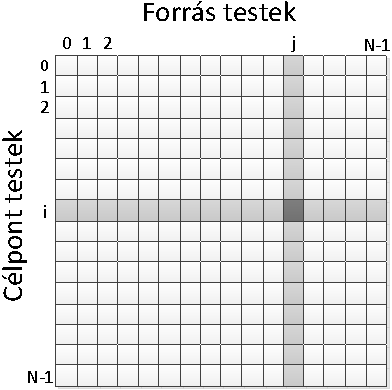
\includegraphics[width=100mm, keepaspectratio]{figures/Implementation/Impl_GPU_Matrix-cropped.pdf}
		\caption{A probl�ma m�trixos elrendez�se}
		\label{fig:Impl_GPU_Matrix}
		\end{figure}

		A CUDA lehet�s�get biztos�t nagyon sok\footnote{Egy r�csban maximum $65536 \cdot 65536 \cdot 65536$ blokk, blokkonk�nt maximum 1024 sz�l. Ez egy elm�leti �rt�k, a rendelkez�sre �ll� hardver er�forr�s korl�tozhat.} sz�l elind�t�s�ra, �gy kernel �r�sakor gyakori megk�zel�t�s lehet, hogy minden sz�l egy apr� r�szm�veletet v�gezzen. A probl�ma lek�pezhet� egy kernelre a fenti form�ban egy az egyben, de k�zel sem fog optim�lis eredm�nyt adni.
		
		Az els� probl�ma, ami szembe j�n, az a mem�ria hozz�f�r�sek sz�ma. Ha minden sz�l csak egy testp�r k�z�tti gyorsul�st sz�mol, akkor egy testet �sszes ki kell olvasni a glob�lis mem�ri�b�l $(2N-2)$-sz�r. Egy test $N$-szer c�lpont, �s $N$-szer hat m�sik testre. A $(-2)$ pedig az �nmag�val vett interkaci�k miatt j�n be. �s b�r rendelkez�sre �ll valamennyi cache, a tranzakci�k sz�ma �gy is nagy, ami h�tr�ltatni fogja a sz�m�t�sokat �s a korl�tot nem a sz�m�t�si kapacit�s fogja jelenteni, hanem a mem�ria s�vsz�less�ge.
	
	%----------------------------------------------------------------------------
	\subsection{Feldarabol�s}
	%----------------------------------------------------------------------------
		Els� l�p�sk�nt �rdemes nagyobb csoportokra (\emph{tile}) bontani a probl�m�t (\figref{Impl_GPU_Tile} �bra). C�lja a feldarabol�snak, hogy az egy az egyben egy TB-hez rendelhet�k legyenek a darabok, melyben elhelyezked� sz�lak k�pesek az egym�s k�z�tti adatmegoszt�sra, ezzel optimaliz�lva a mem�ria hozz�f�r�sek sz�m�t.

		\begin{figure}[!ht]
		\centering
		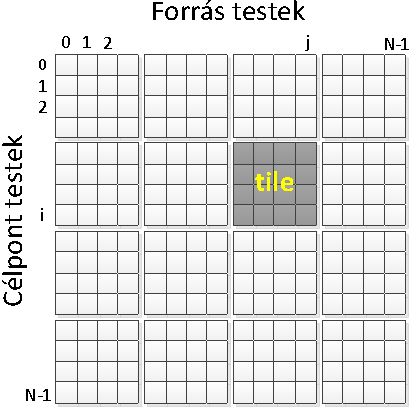
\includegraphics[width=100mm, keepaspectratio]{figures/Implementation/Impl_GPU_Tile-cropped.pdf}
		\caption{Felbontott, tile-os elrendez�s}
		\label{fig:Impl_GPU_Tile}
		\end{figure}

		Az �br�n besz�rk�tett $4\cdot4$-es tile eset�n �sszesen 8 testhez tartoz� inform�ci� egyszeri felhozatala sz�ks�ges, a 16 helyett, ha az adatokat el lehetne t�rolni a blokk �ltal k�z�sen haszn�l \emph{shared mem�ri�ban}. A sz�lak a sz�m�t�st m�r csak akkor kezden� el, amikor minden test adata m�r bet�lt�d�tt oda.
		
		Ezzel cs�kkenteni lehetett a glob�lis mem�ri�hoz val� hozz�f�r�sek sz�m�t, �s egy olyan mem�ri�ba ker�lt a sz�ks�ges inform�ci�, mely p�rhuzamos hozz�f�r�st el�seg�t� bankokba van szervezve. Am�g az egy warp-on bel�li sz�lak m�s-m�s bankhoz pr�b�lnak hozz�f�rni (vagy t�bben egy bankon bel�l ugyanahhoz a rekeszhez), addig j� teljes�tm�nyt lehet el�rni.
	
	%----------------------------------------------------------------------------
	\subsection{P�rhuzamoss�g cs�kkent�se}
	%----------------------------------------------------------------------------
		Az N-test szimul�ci� �s p�ldak�nt felhozott m�trixszorz�s is remek, $N^2$-es p�rhuzamos�t�si lehet�s�get biztos�t, azonban mindk�t esetben sz�ks�ges az egyes r�szeredm�nyek �sszegz�se.
		
		N-test szimul�ci� eset�n ez azt jelenti, hogy minden sz�l kisz�mol egy testp�r k�z�tti interakci� �ltal behozott gyorsul�s�rt�ket, majd egy kijel�lt sz�l/sz�lak csoportja akkumul�lja az eredm�nyeket. Hab�r maga az akkumul�l�s folyamata megval�s�that� $O(logN)$ komplexit�s� redukci�s algoritmussal, a sz�lak k�zti kommunik�ci� �s szinkroniz�ci� igencsak jelent�s. Nem besz�lve az akkumul�ci�t v�gz� kijel�lt sz�lak �ltal behozott sz�ldivergenci�r�l.
		
		Mivel a sz�lon bel�li kommunik�ci�, adatmozgat�s l�nyegesen gyorsabb, mint a sz�lak k�zti, a megold�st az jelentheti, ha minden sz�l egy c�lponthoz tartoz� gyorsul�st sz�mol. Vagyis minden l�trehozott sz�l pontosan $N$ interakci�t hajt v�gre �s akkumul�lja az eredm�nyeket, ezzel cs�kkenthetve a sz�lak k�zti szinkroniz�ci�s �s kommunik�ci�s folyamatok sz�m�t.
		
		�sszesen teh�t $N \cdot N$ sz�l �s a kommunik�ci� intenz�v megold�s helyett, $N$ sz�lat l�trehozva megoldhat� a probl�ma. Az \figref{Impl_GPU_LessParallel} �br�n l�that� bejel�lve az $i.$ sz�l �ltal elv�gzend� sz�m�t�sok, a halad�si ir�nyt felt�ntetve.

		\begin{figure}[!ht]
		\centering
		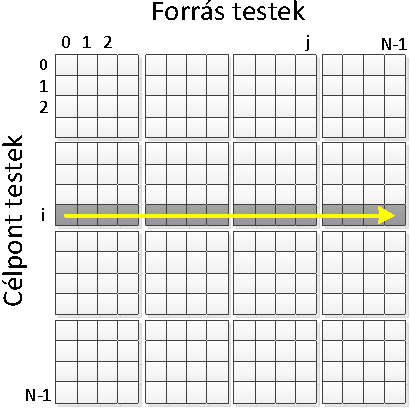
\includegraphics[width=100mm, keepaspectratio]{figures/Implementation/Impl_GPU_LessParallel-cropped.pdf}
		\caption{Az egy sz�l �ltal elv�gzend� feladatok}
		\label{fig:Impl_GPU_LessParallel}
		\end{figure}

		Ezzel a l�p�ssel cs�kkentett�k a feladat p�rhuzamoss�g�t, t�bb munk�t adva egy sz�l sz�m�ra, de cser�be megsz�ntett�k sz�lak k�zti kommunik�ci�t. Kism�ret� szimul�ci�k eset�n nem biztos, hogy ez a megold�s adja a legjobb teljes�tm�nyt. N�h�ny ezer test kell legal�bb, hogy j�l ki legyenek haszn�lva a GPU er�forr�sai.
		
		Egy darabja a m�trixnak (tile), egy TB-nak feleltethet� meg.
	
	%----------------------------------------------------------------------------
	\subsection{Konkl�zi�}
	%----------------------------------------------------------------------------
		A k�t fenti v�ltoztat�st egyberakva, egy TB az \figref{Impl_GPU_TB} �bra alapj�n fog m�k�dni.

		\begin{figure}[!ht]
		\centering
		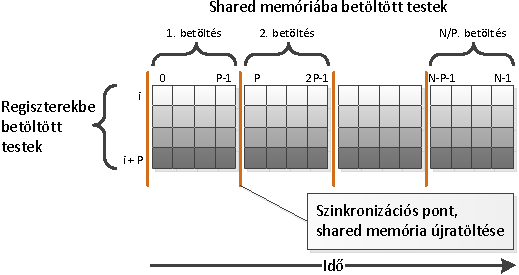
\includegraphics[width=130mm, keepaspectratio]{figures/Implementation/Impl_GPU_TB-cropped.pdf}
		\caption{Egy threadBlock m�k�d�se}
		\label{fig:Impl_GPU_TB}
		\end{figure}

		Minden TB egy dimenzi�s lesz pontosan $P$ darab sz�llal (ez pontosan a $blockDim.x$ be�p�tett v�ltoz� �rt�k�t fogja meghat�rozni). Minden sz�l bet�lti a regisztereibe azt az egy testet, amely minden sz�m�t�s sor�n dolgozni fog. A saj�t be�p�tett $threadIdx.x$ �s az �ppen aktu�lis tile sorsz�ma alapj�n bet�lt egy darab testet a shared mem�ri�ba. Ha j�l van elt�rolva az adat a glob�lis mem�ri�ban, akkor egy warp (32 sz�l) k�pes felhozni egy olvas�ssal $32$ \verb+float+ adatot �s elt�rolni azt bank konfliktus n�lk�l a shared mem�ri�ba.
		
		Ahhoz, hogy a sz�m�t�s elindulhasson, be kell v�rni, m�g minden sz�l bet�lti a hozz�rendelt testet. Ezt \verb+__syncthreads()+ f�ggv�ny seg�ts�g�vel fel�ll�tott szinkroniz�ci�s pontokkal tehetj�k meg. Az azonos TB-n bel�li sz�lak az ilyen pontokn�l mindig bev�rj�k egym�st.
		
		Amint v�get �rt az adott tile-on az gyorsul�s�rt�kek meghat�roz�sa (szint�n szinkroniz�ci� kell), �jrakezd�dik a folyamat a k�vetkez� P darab test bet�lt�s�vel. �sszesen $2 \cdot N/P$ szinkroniz�ci�s pont lesz egy TB fut�sa sor�n.
		
		A k�vetkez� feladat a P �rt�k�nek meghat�roz�sa. Ehhez figyelembe kell venni az eszk�z�nk param�tereit is. Ha P �rt�ke t�l kicsi, az azt eredm�nyezi, hogy az esetemben egy SM-en elhelyezhet� maxim�lis 8 TB fog korl�toz� t�nyez� lenni, �s a rendelkez�sre �ll� regiszterek, shared mem�ria, stb. nem lesznek kihaszn�lva. Ha P �rt�ke nagy (maximum 1024), akkor meg m�s korl�toz� t�nyez� fog k�zbesz�lni (pl.: regiszterek), melyek miatt kevesebb, mint 8 TB-t tud csak egy SM-en bel�l p�rhuzamosan l�tezni.
		
		Kell keresni egy k�z�putat. Ezt els�sorban k�s�rletez�ssel lehet megtenni. �k�lszab�lyk�nt elmondhat�, hogy a TB-ben l�v� sz�lak sz�ma legyen a 32-nek eg�sz sz�m� t�bbsz�r�se, �s legal�bb 128. �gy el�rhet�, hogy az eszk�z a lehet� legjobban le legyen foglalva (occupancy). Sosem szabad teljes m�rt�kben a foglalts�got szem el�tt tartani, ugyanis lehet, hogy egy kisebb occupancy-val rendelkez� nagyobb kernel jobb teljes�tm�nyt ny�jt. Az alacsony ($50\%$ alatti) viszont val�sz�n�, hogy nem az ide�lis eredm�nyt adja.
	
	%----------------------------------------------------------------------------
	\subsection{A k�d}
	%----------------------------------------------------------------------------
		Az \figref{Impl_Algorithm} �br�n l�that� fel�p�t�st k�vetve, el�sz�r a \verb+NBodyAlgorithmGPU+ oszt�ly megval�s�t�s�t kezdtem el. �gy terveztem, hogy \verb+__device__+ jelz�vel rendelkez�, egym�st�l j�l elk�l�n�thet� f�ggv�nyeket hozok l�tre. Ez a \verb+__global__+ kernel jelz�h�z hasonl� szerepet t�lt be. Megjel�li, hogy az adott f�ggv�ny csak egy GPU-n futtatand� kernelb�l h�vhat�.
	
		\verb+Body+ oszt�ly haszn�lata helyett kicsomagoltam \verb+float3+, \verb+float+ �s \verb+float4+ t�mb�kbe az attrib�tumokat a jobb teljes�tm�ny, mem�ria- �s regiszter felhaszn�l�s �rdek�ben.
	
		T�bb kernelt megval�s�tottam, hogy �ssze tudjam hasonl�tani, milyen m�don tudom el�rni a legjobb teljes�tm�nyt. Ebb�l a legjobb fut�si id�vel rendelkez�t mutatom be.
		
		El�sz�r sz�pen \verb+float3+-mal pr�b�lkoztam a poz�ci��rt�kek �s \verb+float+-tal a t�megek elt�rol�s�ra, de egy jobb megold�snak bizonyul, ha \verb+float4+-et alkalmazok. Ennek oka lehet, hogy glob�lis mem�ri�ban a \verb+float4+-ek kit�ltenek egy teljes szegmenst, m�g a \verb+float3+-ak nem. Ez�rt \verb+float3+-n�l t�bb szegmens kiolvas�sa t�rt�nhet meg, ha a sz�ks�ges adat k�t szegmensbe is bel�g. A \verb+float4+ negyedik mez�j�ben (w) ker�lt elt�rol�sra a t�meg.

		\begin{lstlisting}
__device__ float3 calculateAccelerationWithFloat4(float4 posI, float4 posJ, float3 accI) {
	float3 r;

	// A k�t test t�vols�gvektora
	r.x = posJ.x - posI.x;
	r.y = posJ.y - posI.y;
	r.z = posJ.z - posI.z;


	// A k�t test skal�ris t�vols�ga
	float rabs = sqrt(r.x * r.x + r.y * r.y + r.z * r.z + d_EPS2);

	// A k�plet nevez�je
	float rabsInv = 1.0f / (rabs * rabs * rabs);
	float temp = posJ.w * rabsInv;

	// MAC m�velet, gyorsul�s meghat�roz�sa
	accI.x += r.x * temp;
	accI.y += r.y * temp;
	accI.z += r.z * temp;

	return accI;
}
		\end{lstlisting}
	
		A k�d nagyon hasonl�t a referencia megval�s�t�sra, azonban a kor�bbiakhoz k�pest a \verb+calculateAcceleration+ v�gzi el a gyorsul�s�rt�kek akkumul�l�st is. Szorz�s �s �sszegz�s (MAC - Multiply and Accumulate) m�velet egy utas�t�st tesz ki, valamint dedik�lt v�grehajt� egys�ge is van, �gy nem �rdemes sz�tv�lasztani �ket.
		
		A \verb+d_EPS2+ egy az eszk�z konstans mem�ri�j�ban elt�rolt �rt�k.
		
		\begin{lstlisting}
__device__ float3 advanceWithFloat4(float4 posI, float4 *g_pos) {
	extern __shared__ float4 sh_pm[];

	//Akkumul�tor
	float3 accI = { 0.0f, 0.0f, 0.0f };

	// Tile-ok iter�ci�ja
	for (int i = 0, tile = 0; i < d_NUM_BODY; i += blockDim.x, tile++) {
		// Bet�ltend� adat poz�ci�j�nak meghat�roz�sa
		int tileID = tile * blockDim.x + threadIdx.x;

		// Poz�ci� �s t�meg bet�lt�se a meghat�rozott tileID alapj�n
		sh_pm[threadIdx.x] = g_pos[tileID];

		//Szinkroniz�ci�s pont: shared mem�ria t�lt�se
		__syncthreads();   

		// Tile-okon bel�li interakci�k kisz�m�t�sa
		#pragma unroll 128
		for (int j = 0; j < blockDim.x; j++) {
			accI = calculateAccelerationWithFloat4(posI, sh_pm[j], accI);
		}
		//Szinkroniz�ci�s pont: sz�m�t�sok v�ge
		__syncthreads();    
	}

	return accI;
}
		\end{lstlisting}

		Az \verb+advanceWithFloat4+ f�ggv�nyben tartja sz�mon a sz�l, hogy �ppen megint tile elemein kell elv�gezni a sz�m�t�sokat. Minden sz�l a meghat�rozott \verb+tileID+ alapj�n kikeresi a sz�m�ra bet�ltend� testet, �gy egy TB-n bel�l egy sz�l pontosan 1 elem�t t�lti be az osztott mem�ri�ba. A m�sol�st k�vet�en l�that� az els� szinkroniz�ci�s pont, melynek c�lja, hogy a sz�lak bev�rj�k az �sszes test bet�lt�d�s�t. A sz�m�t�st k�vet�en l�that� a m�sodik szinkroniz�ci�, mely a k�vetkez� tile-ra l�p�st, �s ezzel az osztott mem�ria �jrat�lt�s�t akad�lyozza, m�g van sz�m�t�st v�gz� sz�l.
	
		A m�g kiemelend� r�sz az \verb+extern+ \verb+__shared__+ \verb+float4+ \verb+sh_pm[]+ sor. Ez a shared mem�ri�t reprezent�l� v�ltoz�. Az \verb+extern+ kulcssz� jel�li meg, hogy az adott v�ltoz� m�rete k�v�lr�l ker�l be�ll�t�sra, fut�si id�ben. Ezt a kernel futtat�si konfigur�ci�j�n�l kell megadni, a TB m�ret�nek megad�sa ut�n. A \verb+__shared__+ jel�li, hogy az osztott mem�ri�ban helyezkedik el a \verb+sh_pm+ v�ltoz�.
	
		El�sz�r k�l�n shared v�ltoz�t szerettem volna l�trehozni a t�meg �s a poz�ci�k sz�m�ra, de a futtat�si param�terekben csak egy t�mbnek lehet megadni a m�ret�t, a m�sodik pedig az els� ter�let�re fog mutatni. Ez is indokolta a \verb+float4+ t�pus haszn�lat�t a glob�lis mem�ria szegmensei mellett.
		
		Shared mem�ria megfelel� haszn�lat�nak egy fontos eleme a bankkonfliktus elker�l�se, mely sor�n biztos�tjuk, hogy a warp-on bel�li sz�lak, m�s-m�s bank 32 bites rekeszeihez f�r�nk hozz�. Ez a fenti k�dban a \verb+float4+ haszn�lata miatt sajnos nem teljes�l.

		% Table generated by Excel2LaTeX from sheet 'Bank konfliktus'
		\begin{table}[htbp]
		  \centering
		  \caption{Float4 t�mb elhelyezked�se shared mem�ri�ban}
			\begin{tabular}{|l|l|l|l|l|l|l|l|l|l|l|l|l|l|l|l|}
			\hline
			Bank  & 0 & 1 & 2 & 3 & 4 & 5 & 6 & 7 & 8 & 9 & ...     & 30 & 31 & 0 & 1 \\
			\hline
			Test  & 0 & 0 & 0 & 0 & 1 & 1 & 1 & 1 & 2 & 2 &...     & 7 & 7 & 8 & 8 \\
			\hline
			Adat  & x     & y     & z     & w     & x     & y     & z     & w     & x     & y     & ...     & z     & w     & x     & y \\
			\hline
			\end{tabular}%
		  \label{tab:GPU_shared_float4}%
		\end{table}%

		Els� tranzakci� sor�n a testek poz�ci�j�nak $x$ koordin�t�ja ker�l be�r�sra, ugyanis warpon bel�li sz�lak k�t�tten, egyszerre ker�lnek v�grehajt�sra. A $0.$ sz�l be�rja $0.$ test poz�ci�j�nak $x$ koordin�t�j�t a $0.$ bankba, azonban az $1.$ sz�l nem a soron k�vetkez�t fogja �rni, hanem a $4$-et. Ez a hozz�f�r�st eltolt (strided) hozz�f�r�snek is nevezik. A probl�m�t a $8.$ sz�l fogja okozni. Az �ltala �rt rekesz ugyanis a $0.$ sz�l �ltal hozz�f�rt $0.$ bankban helyezkedik el. A l�nc folytat�dik tov�bb, �gy bel�that�, hogy a 32 bankb�l mind�ssze 8 lesz kihaszn�lva. A tov�bbi koordin�t�k �s a t�meg �r�s�n�l is ez t�rt�nik. Eltolt hozz�f�r�s eset�n akkor oldhat� fel teljes eg�sz�ben a bankkonfliktus, ha az eltol�s m�rt�ke egy p�ratlan sz�m. A \verb+float3+ t�pus viszont osztott mem�ria eset�n sokkal kedvez�bb.

		% Table generated by Excel2LaTeX from sheet 'Bank konfliktus'
		\begin{table}[htbp]
		  \centering
		  \caption{Float3 t�mb elhelyezked�se shared mem�ri�ban}
			\begin{tabular}{|l|l|l|l|l|l|l|l|l|l|l|l|l|l|l|l|}
			\hline
			Bank  & 0 & 1 & 2 & 3 & 4 & 5 & 6 & 7 & 8 & 9 & ...     & 30 & 31 & 0 & 1 \\
			\hline
			Test  & 0 & 0 & 0 & 1 & 1 & 1 & 2 & 2 & 2 & 3 &...     & 10 & 10 & 10 & 11 \\
			\hline
			Adat  & x     & y     & z     & x     & y     & z     & x     & y     & z     & x     & ...     & x     & y     & z     & x \\
			\hline
			\end{tabular}%
		  \label{tab:GPU_shared_float3}%
		\end{table}%

		A glob�lis mem�ria olvas�sa �s a szegmenshat�rok betart�sa miatt azonban teljes�tm�nyben l�nyegesen jobban teljes�t ez a kernel. A bankkonfliktusok felold�sa priorit�sban alacsonyabb poz�ci�t foglal el, mint a glob�lis mem�ria s�vsz�less�g optimaliz�l�sa, tekintve, hogy ut�bbi j�val nagyobb hat�ssal van a kernel fut�si teljes�tm�ny�re.
	
		A bels� \verb+for+ ciklus eleinte egy k�l�n f�ggv�ny, de egy id� ut�n zavar�nak tartottam, �gy kiszedtem. Az \verb+unroll+ hat�s�ra n�vekedik a k�d m�rete, �s a felhaszn�lt regiszterek sz�ma, ami azt eredm�nyezi, hogy kevesebb TB fog elf�rni egyszerre egy SM-en bel�l, de az �sszteljes�tm�ny n�vekedett.
		
		\begin{lstlisting}
__global__ void integrateKernelWithFloat4(float4 *g_posOld, float4 *g_posNew, float4 *g_vel) {
	// A c�lpont test sorsz�m�nak meghat�roz�sa
	int globalThreadID = blockIdx.x * blockDim.x + threadIdx.x;

	// A felesleges sz�lak deaktiv�l�sa
	if (globalThreadID > d_NUM_BODY) return;

	float stepTime2 = 0.5f * d_STEP_TIME * d_STEP_TIME;

	// C�lpont test adatainak beolvas�sa regiszterekbe
	float4 posI = g_posOld[globalThreadID]; // coalesced
	float4 velI = g_vel[globalThreadID];    // coalesced
	float3 accI;

	accI = advanceWithFloat4(posI, g_posOld);

	// Poz�ci� friss�t�se
	posI.x += velI.x * d_STEP_TIME; +accI.x * stepTime2;
	posI.y += velI.y * d_STEP_TIME; +accI.y * stepTime2;
	posI.z += velI.z * d_STEP_TIME; +accI.z * stepTime2;

	// Sebess�g friss�t�se
	velI.x = velI.x * d_VELOCITY_DAMPENING + accI.x * d_STEP_TIME;
	velI.y = velI.y * d_VELOCITY_DAMPENING + accI.y * d_STEP_TIME;
	velI.z = velI.z * d_VELOCITY_DAMPENING + accI.z * d_STEP_TIME;

	// Eredm�nyek visszaolvas�sa a glob�lis mem�ri�ba
	g_posNew[globalThreadID] = posI;
	g_vel[globalThreadID] = velI;
	//g_acc[globalThreadID] = accI;
}
		\end{lstlisting}

		A kernel el�sz�r a sz�l sorsz�m�nak meghat�roz�s�val kezd�dik. Ez egyben meghat�rozza, hogy melyik testnek kell kisz�molnia az adatait. Amennyiben t�bb sz�lat ind�tottunk, mint amennyi test�nk van, a felesleges sz�lak deaktiv�l�sra ker�lnek. Ilyen helyzet �ll el�, ha a testek sz�ma nem oszthat� a TB-ben l�v� sz�lak sz�m�val.
	
		A sz�lak �ltal k�z�sen haszn�lt v�ltoz�k \verb+d_NUM_BODY+, \verb+d_VELOCITY_DAMPENING+, \verb+d_STEP_TIME+ mindegyike konstans mem�ri�ban vannak elt�rolva. Kisz�m�t�sra ker�l a \verb+steptime+ n�gyzete, ami egy kezdetlegesebb kernel hagyat�ka, �s �gy ut�lag belegondolva c�lszer�bb lett volna konstans mem�ri�ba bet�lteni a host-b�l. Eleinte azonban probl�m�k ad�dtak a konstans mem�ria haszn�lat�val. Egyr�szt oszt�ly tagv�ltoz�jak�nt nem lehet deklar�lni, ford�t�si id�ben l�teznie kell, m�sr�sz az �soszt�ly header f�jlj�ban deklar�lva, a \verb+cudaMemcpyToSymbol+ (konstans mem�ri�ba m�sol�s) nem tudott bele �rt�ket �rni.
	
		A c�lpont adatait egyszer� v�ltoz� deklar�ci�val �s �rt�kad�ssal belerakjuk a gyors hozz�f�r�s� regiszterekbe. Ha a regiszterek elfogytak, akkor ker�l haszn�latra a lass�, de cache-sel rendelkez� lok�lis mem�ria. Mivel az azonos t�pus� elemek egy t�mb�t alkotnak �s nem test szerint vannak a glob�lis mem�ri�ban rendezve az adatok, a \verb+float4+ �rt�kek kiolvas�sa \emph{coalesced}. Ez azt jelenti, hogy warp-on bel�li sz�lak sorfolytonos mem�riarekeszekhez szeretn�nek hozz�f�rni, �gy minimaliz�lva a sz�ks�ges mem�ria tranzakci�k sz�m�t. Ha \verb+Body+ strukt�r�k t�mbje lenne a glob�lis mem�ri�ba m�solva, akkor a kiolvas�s \emph{strided} lenne, melynek eredm�nye, hogy az adott pillanatban felesleges, t�meg, gyorsul�svektor �s sebess�gvektor is beolvas�sra ker�l. Ezzel a felhozott mem�riaszegmensek sz�ma l�nyegesen nagyobb lenne.
	
		A kisz�molt adatok vissza�r�sa felvet egy probl�m�t. Mivel az egyes sz�lak, egym�st�l f�ggetlen�l (kommunik�ci� n�lk�l) futnak, ez�rt az �j poz�ci��rt�kek vissza�r�sa gondot jelent. El�fordulhat olyan helyzet, hogy egy sz�l m�r befejezte a m�k�d�s�t, vissza�rta az eredm�nyt, de egy m�sik sz�l m�g csak akkor kezdi a sz�m�t�s�t. Ahhoz, hogy mindig konzisztens adatokkal tudjanak dolgozni, a k�z�sen felhaszn�lt poz�ci�vektorokat bufferelni kell. Kell k�t \verb+float4+ t�mb a glob�lis mem�ri�ban, melyek k�z�l az egyiket csak olvassa, a m�sikat pedig csak �rja a kernel. Kernel �jrah�v�sakor (a k�vetkez� iter�ci� kezdet�n) a host a k�t buffert kicser�li: amit legut�bb �rt a kernel, azt fogja olvasni.
	
		A nagyobb fut�si sebess�g el�r�s�hez gyorsul�svektor vissza�r�sa ki van kommentezve a fenti k�dban, mert az �rt�ke minden iter�ci�ban fel�l lesz �rva. A host oldal pedig jelenleg nem dolgozik a kisz�molt �rt�kekkel, a megjelen�t�s �s a referenciamodell sz�m�ra csak a poz�ci��rt�kek a relev�nsak.

		\begin{lstlisting}
...
integrateKernelWithFloat4 <<< m_gridSize, m_threadBlockSize, m_sharedMemorySize >>> (mpd_position4[1 - m_writeable], mpd_position4[m_writeable], mpd_velocity4);

// Kernelh�v�s st�tusz�nak ellen�rz�se
cudaError_t kernelStatus = cudaGetLastError();
if (kernelStatus != cudaSuccess) {
	std::cerr << "Kernel launch failed: " << cudaGetErrorString(kernelStatus) << std::endl;
}

// V�rakoz�s a kernel befejez�s�re
checkCudaError(cudaDeviceSynchronize());

// Poz�ci��rt�kek visszaolvas�sa tov�bbi feldolgoz�sa
checkCudaError(cudaMemcpy(mph_position, mpd_position[m_writeable], mp_properties->numBody * sizeof(float3), cudaMemcpyDeviceToHost));
checkCudaError(cudaMemcpy(mph_position4, mpd_position4[m_writeable], mp_properties->numBody * sizeof(float4), cudaMemcpyDeviceToHost));

// �rt�k invert�l�s, buffer v�lt�sa
m_writeable = 1 - m_writeable; 
...
		\end{lstlisting}

		A kernel konfigur�ci�s list�j�ban szerepel $3.$ param�terk�nt a shared mem�ria m�rete b�jtokban megadva. Ennek �rt�ke a futtatand� sz�lak sz�m�t�l f�gg�en v�ltozik. 256 sz�l eset�n, egyszerre 256 test adatai lesznek bet�ltve a shared mem�ri�ba, �gy $256 \cdot 4 \cdot sizeof(float)$, azaz 4 kB lesz.
	
		Az argumentumban l�that� a dupla bufferel�s megold�sa. Az \verb+m_writeable+ v�ltoz� $0$ vagy $1$ �rt�ket vehet, ezzel megszabva, hogy a kernelben melyik \verb+mpd_position4+ lesz az �j, melyik a r�gi �rt�keket t�rol� t�mb. Az eredm�nyek visszam�sol�s�t k�vet�en t�rt�nik a bufferek v�lt�sa az \verb+m_writeable+ �rt�k�nek invert�l�s�val.
	
		Az egyes CUDA f�ggv�nyh�v�sok el�tt l�that� egy \verb+checkCudaError+ nev� \verb+define+, mely az al�bbi k�dr�szlet szerint ellen�rzi, hogy a visszat�r�si �rt�k \verb+cudaSuccess+-e. Amennyiben elt�r�st tapasztal, lek�rdezi a hiba ok�t, ki�rja azt, majd kil�p a programb�l.

		\begin{lstlisting}
#define checkCudaError(ans) { gpuAssert((ans), __FILE__, __LINE__); }
inline void gpuAssert(cudaError_t code, const char *file, int line, bool abort = true) {
	if (code != cudaSuccess) {
		std::cerr << "CUDA failure: " << cudaGetErrorString(code) << " in " << file << " at line " << line << std::endl;
		if (abort)
			exit(code);
	}
}
		\end{lstlisting}
		
		A kernel m�ret�t a \verb+setKernelParameters+ f�ggv�ny csin�lja, mely beolvassa a rendelkez�sre �ll� GPU inform�ci�it �s az alapj�n pr�b�l egy legal�bb $75\%$-os kihaszn�lts�g� futtat�si konfigur�ci�t be�ll�tani. Ez volt a tervem legal�bbis. A nagysz�m� regisztereket haszn�l� kernelem azonban ezt megnehez�tette. Pr�b�lkoz�sok sor�n a legjobb eredm�nyt a 256 sz�llal rendelkez� TB-ok adt�k. A TB-ok darabsz�m�t (r�cs m�ret�t) a testek sz�ma osztva a TB m�ret�vel adja ki.
	
		A kernel fut�s�nak v�g�t a \verb+cudaDeviceSynchronize+ f�ggv�ny seg�ts�g�vel tudjuk bev�rni, lehet�v� t�ve, hogy az eredm�nyek visszam�solhat�k legyenek.
		
	%----------------------------------------------------------------------------
	\subsection{Probl�m�k}
	%----------------------------------------------------------------------------
		%----------------------------------------------------------------------------
		\subsubsection{Watchdog}
		%----------------------------------------------------------------------------
			Ha a szimul�ci� tov�bb tartott, mint $2$ m�sodperc a Windows watchdog-szer� m�k�d�s szerint �jraind�totta, alaphelyzetbe �ll�totta a videok�rtya drivert, �s vele egy�tt a GPU-t. Ezt a registry-ben tal�lhat� hat�r�rt�k m�dos�t�s�val kik�sz�b�ltem.
		
		%----------------------------------------------------------------------------
		\subsubsection{NSight Debugger}
		%----------------------------------------------------------------------------
			Technikai probl�m�ba �tk�ztem, amikor a GPU kernelt debugolni pr�b�ltam. Folyton hiba�zenettel v�get �rt a debug m�d:
			\begin{quote}
				CUDA context was created on a GPU that is not currently debuggable.
			\end{quote}
			A sz�m�t�g�pemben tal�lhat� kett� GPU k�z�l csak az egyik CUDA kompatibilis, a m�sik egy integr�lt Intel GPU. Az NVIDIA NSight debugger, akkor m�k�dik, ha a kijelz� vez�rl�s�t nem a vizsg�lat alatti GPU v�gzi.
			
			El�sz�r megpr�b�ltam a megjelen�t�st kiz�r�lagosan az integr�lt Intel GPU-ra b�zni, �m ez nem seg�tett. Azt�n k�ls� javaslatok alapj�n friss�tettem a CUDA-t 7.0-r�l 8.0-ra, ezzel egy�tt az NSight debuggert 4.5-r�l 5.2-re. Ezzel egy�tt a driver friss�t�se is sz�ks�gess� v�lt, ugyanis az �j NVCC-vel ford�tott k�dot nem tudta futtatni.
			
			Minden er�fesz�t�sem ellen�re nem siker�lt m�k�d�sre b�rni az NSight debuggert. Maradtam a r�gi m�dszern�l, hogy ki�ratom a v�ltoz�k �rt�k�t konzolra.


%----------------------------------------------------------------------------
\chapter{Ellen�rz�s}
%----------------------------------------------------------------------------
	Az els� ellen�rz�si forma, amit megval�s�tottam az az OpenGL alap� grafikus megjelen�t�s. Ezzel k�nnyen felder�thet�, ha valamelyik k�plet implement�l�sa sor�n hib�t v�tettem. Ezt k�vet�en l�trehoztam az \verb+NBodySystem+ oszt�lyon bel�l a referencia algoritmus p�ld�nyos�t�s�hoz sz�ks�ges v�ltoz�kat. Kieg�sz�tettem a szimul�ci�t a referencia iter�ci�val, valamint a testek poz�ci�j�t ellen�rz� f�ggv�ny megh�v�s�val.
	%----------------------------------------------------------------------------
	\section{Megjelen�t�s}
	%----------------------------------------------------------------------------
		Eleinte 3D-s megjelen�t�st szeretettem volna megval�s�tani, de sajnos az id�m nem engedte, illetve nem is ezen volt a diplomamunk�m hangs�lya. A szimul�tor jelleget fenntartva, azonban igyekeztem jav�tani a l�tv�nyon, a testek s�r�s�galap� kisz�nez�s�vel, valamint k�l�nb�z� kezdeti felt�telek megad�s�nak lehet�s�g�vel. Az XXX �br�n egy n�h�ny felv�tel a program fut�s�r�l grafikus m�dban.

		[K�P: Sorozatk�p n�h�ny szimul�ci�r�l]
	
	%----------------------------------------------------------------------------
	\section{Hibasz�m�t�s}
	%----------------------------------------------------------------------------
		Referenciamodell haszn�lata sor�n felt�telezz�k, hogy az egy sz�lon fut� CPU-s megval�s�t�s eredm�nyei a helyesek. Az �sszehasonl�t�st v�gz� f�ggv�ny az \verb+NBodyUtility+ oszt�lyban kapott helyet. K�t testeket t�rol� t�mb�t hasonl�t �ssze poz�ci�adatok alapj�n, az els� nagyobb elt�r�sn�l, kijelzi az elt�r�s �rt�k�t �s kil�p.
		
		A CPU-s modellek eredm�nyei teljes m�rt�kben megegyeztek. Elt�r�s el�sz�r a CPU-s �s GPU-s megold�sok k�z�tt mutatkozott. Ennek oka a lebeg�pontos sz�m�t�sok hardveres megval�s�t�s�ban keresend� \cite{CUDAFloat}.
		
		\begin{itemize}
			\item GPU rendelkezik szorz�s-�sszegz�s (MAC) elv�gz�s�re alkalmas hardverrel, m�g a CPU nem. Ezzel az egyes utas�t�sokat m�s sorrendbe rakhatja a ford�t� optimaliz�l�s sor�n.
			\item CPU pontosabb sz�m�t�si eredm�nyeket produk�lhat, ugyanis gyakran hosszabb lebeg�pontos mantissz�val dolgozik.
			\item A hib�kat ezenk�v�l m�g kerek�t�sbeli elt�r�s is okozhatja.
		\end{itemize}
		
		A hiba halmoz�d�s�val az elt�r�s minden iter�ci�val n�vekszik �s egy id� ut�n igencsak sz�mottev�v� v�lik.
		
		
		% The GPU has fused multiply-add while the CPU does not. Parallelizing algorithms may rearrange operations, yielding different numeric results. The CPU may be computing results in a precision higher than expected. Finally, many common mathematical functions are not required by the IEEE 754 standard to be correctly rounded so should not be expected to yield identical results between implementations.

%----------------------------------------------------------------------------
\chapter{Eredm�nyek ki�rt�kel�se}
%----------------------------------------------------------------------------
	A szimul�ci�t lefuttattam, minden felhaszn�lt technol�gi�val, illetve kombin�ci�ikkal, az XXX t�bl�zat szerinti param�terez�ssel.
	
	[T�bl�zat]
	
	A m�r�sek tiszt�n csak az iter�ci�kat tartalmazz�k, az program kezdeti inicializ�ci�s f�zis�t nem, mely nagy testsz�m eset�n sok�ig is eltarthat.
	
	Az XXX �br�n l�that� az egyes implement�ci�k �ltal ny�jtott

	[K�P: Lebeg�pontos m�veletv�gz�s teljes�tm�nye] vagy [K�P: M�sodpercenk�nti iter�ci�k sz�ma (FPS)]

	[K�P: Fut�si id�k �sszehasonl�t�sa]

	\section{CPU}
		% Elm�leti hat�r???
		% OpenMP Hyperthread nem ad mindig jobb eredm�nyt mint a 4x-es n�veked�s
		A referenciamodellem gyorsan el�rte a fut�si teljes�tm�ny�nek hat�r�t
		
	\section{GPU}
		A rendelkez�semre �ll� NVIDIA GeForce 525M elm�leti teljes�tm�ny�t a k�vetkez� �sszef�gg�s alapj�n kaphatjuk meg:
		
		\begin{align}
			P_T = \frac{n \cdot f \cdot 2}{1000}
		\end{align}
		
		Ahol $n$ jel�li a CUDA magok sz�m�t, $f$ az �rajel�k frekvenci�j�t. A $2$ szorz� az �rajel ciklusonk�nt v�grehajtott 2 darab utas�t�s miatt j�n be.
		A legt�bb test amivel a szimul�ci�t lefuttattam az 32768 test volt, amin�l 49 GFLOPS sz�m�t�si teljes�t�nyt siker�lt el�rnem. A elm�leti korl�tnak ez sajnos csak k�zel a fele.
		% Elm�leti hat�r 110 GFLOPS
		Theorethical peak performance [GFLOPS] = num of Core * Core clk[MHz] * 2 / 1000
			2, mert 2 utas�t�st hajt v�gre �rajel ciklusonk�nt
			1000 a nagys�grend miatt.
		% Profiler eredm�nyek bemutat�sa
		
		Az eredm�nyekb�l l�that�, hogy alacsony testsz�m (sz�lsz�m) mellett a GPU nem teljes�tett kiemelked�en.


%----------------------------------------------------------------------------
\chapter{�sszefoglal�s}
%----------------------------------------------------------------------------

%----------------------------------------------------------------------------
\chapter*{K�sz�netnyilv�n�t�s}\addcontentsline{toc}{chapter}{K�sz�netnyilv�n�t�s}
%----------------------------------------------------------------------------
	Ez�ton szeretn�m kifejezni k�sz�netemet �s tiszteletemet mindenkinek, aki a diplomamunk�m elk�sz�t�s�hez nagyban hozz�j�rult.
	\newline
	
	K�sz�n�m az elm�lt egy �ves munk�j�t, szakmai tan�csait �s seg�t�k�sz hozz��ll�s�t konzulensemnek, Dr. Dud�s �kos egyetemi adjunktusnak.
	\newline
	
	K�l�n k�sz�nettel tartozom Sverteczky Marcell, T�th G�bor, Kiss Tam�s �s \mbox{Viola Timon} hallgat�t�rsaimnak �s bar�taimnak, akik dolgozatom alapos ellen�rz�s�vel, valamint javaslataikkal el�seg�tett�k annak elk�sz�l�s�t.
	\newline
	
	V�g�l, de nem utols� sorban szeretn�m megragadni az alkalmat arra, hogy kifejezzem h�l�mat �s k�sz�netemet csal�domnak, k�l�n�sen sz�leimnek, akiknek szeretete �s mindennapos t�mogat�sa v�gigk�s�rt egyetemi tanulm�nyaim sor�n.

%\listoffigures\addcontentsline{toc}{chapter}{�br�k jegyz�ke}
%\listoftables\addcontentsline{toc}{chapter}{T�bl�zatok jegyz�ke}

\bibliography{mybib}
\addcontentsline{toc}{chapter}{Irodalomjegyz�k}
\bibliographystyle{ieeetr}

%----------------------------------------------------------------------------
\appendix
%----------------------------------------------------------------------------
	\chapter*{F�ggel�k}\addcontentsline{toc}{chapter}{F�ggel�k}
	\setcounter{chapter}{6}  % a fofejezet-szamlalo az angol ABC 6. betuje (F) lesz
	\setcounter{equation}{0} % a fofejezet-szamlalo az angol ABC 6. betuje (F) lesz
	%\numberwithin{equation}{section}
	%\numberwithin{figure}{section}
	%\numberwithin{lstlisting}{section}
	%\numberwithin{tabular}{section}

%----------------------------------------------------------------------------
%\section{Fut�si eredm�nyek}
%----------------------------------------------------------------------------

	\begin{figure}[!ht]
		\centering
		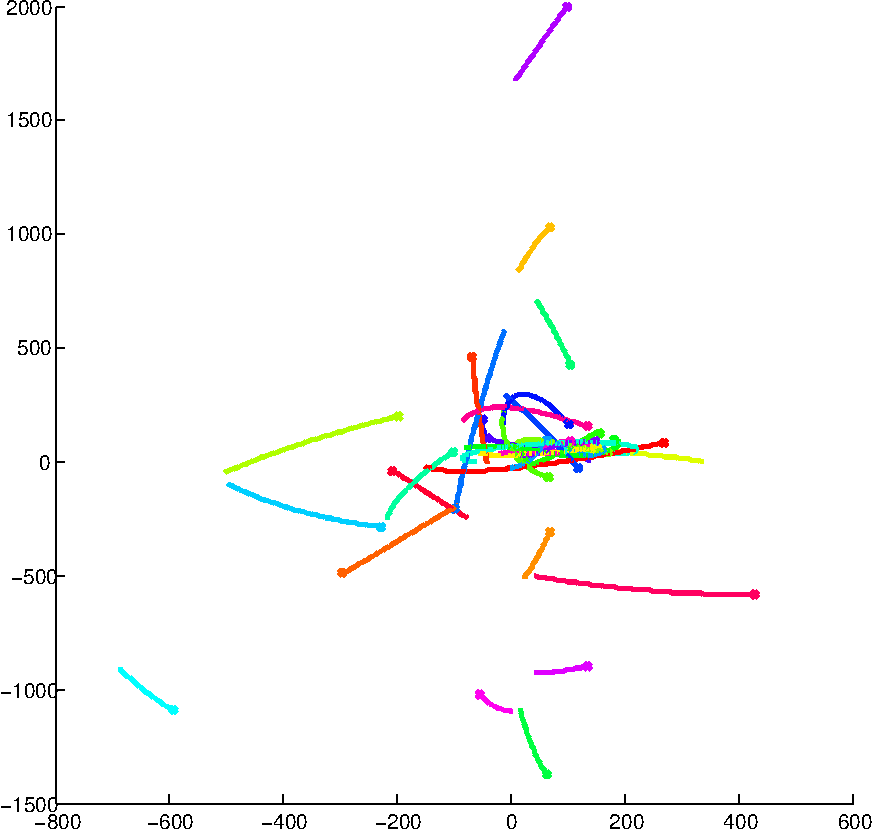
\includegraphics[width=150mm, keepaspectratio]{figures/MATLAB/32_direct-cropped.pdf}
		\caption{Direkt algoritmus �s saj�t integr�tor fut�si eredm�nye MATLAB-ban}
		\label{fig:32_direct}
	\end{figure}
	
	\begin{figure}[!ht]
		\centering
		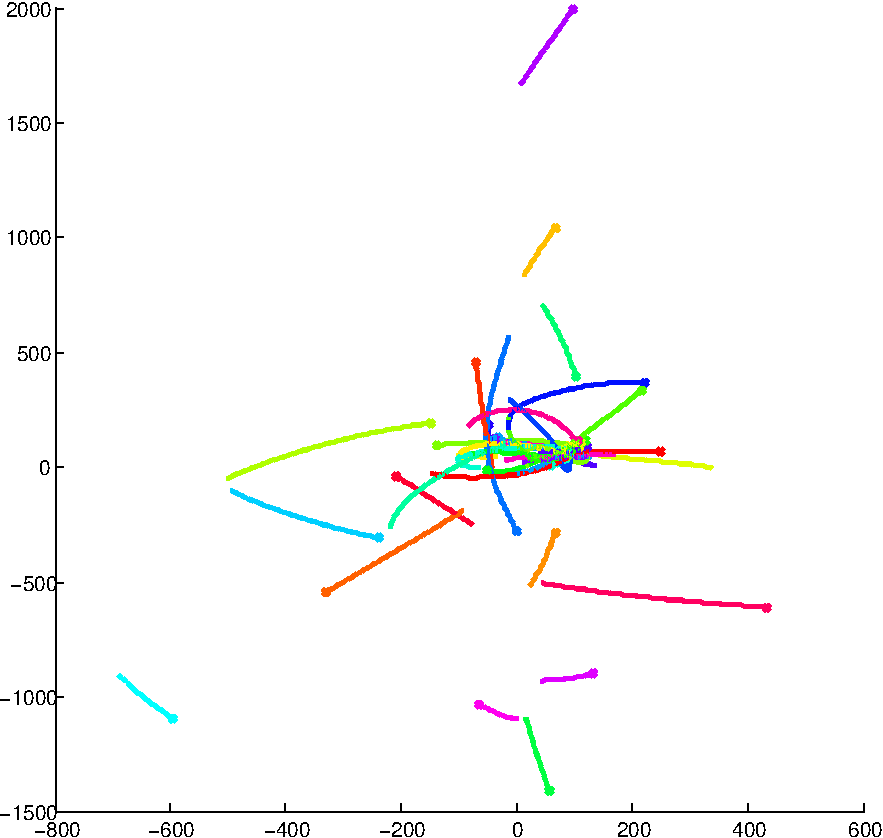
\includegraphics[width=150mm, keepaspectratio]{figures/MATLAB/32_ODE-cropped.pdf}
		\caption{Direkt algoritmus �s KDE megold� fut�si eredm�nye MATLAB-ban}
		\label{fig:32_ODE}
	\end{figure}
	
	\begin{figure}[!ht]
		\centering
		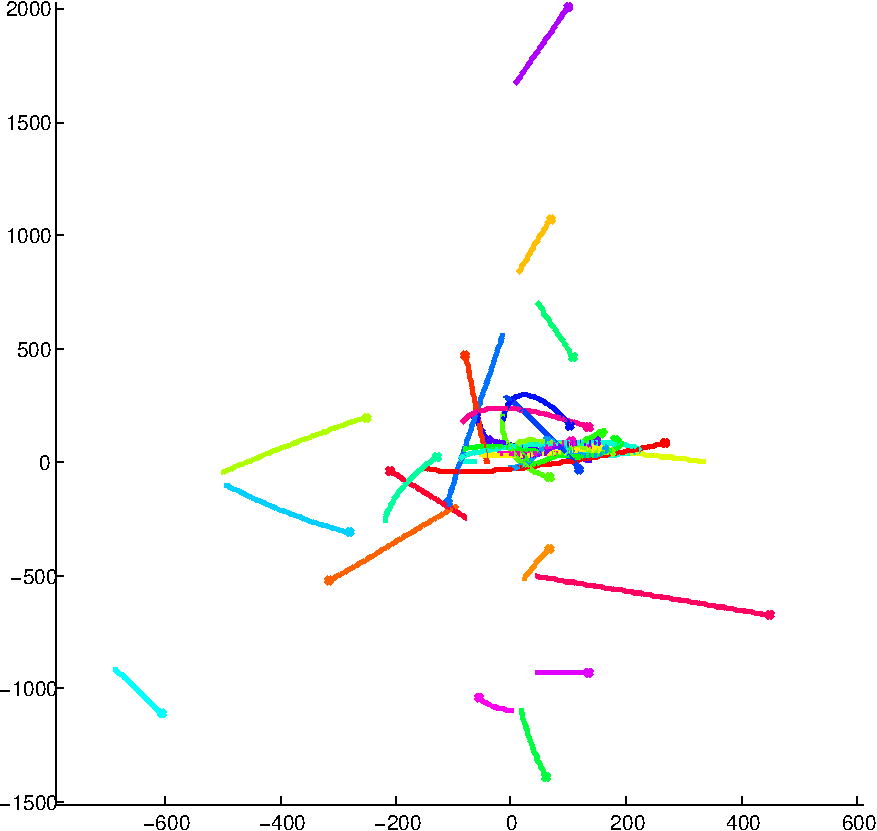
\includegraphics[width=150mm, keepaspectratio]{figures/MATLAB/32_selective-cropped.pdf}
		\caption{K�zel�t� direkt algoritmus �s saj�t integr�tor fut�si eredm�nye \mbox{MATLAB-ban}}
		\label{fig:32_selective}
	\end{figure}


	\begin{figure}[!ht]
		\centering
		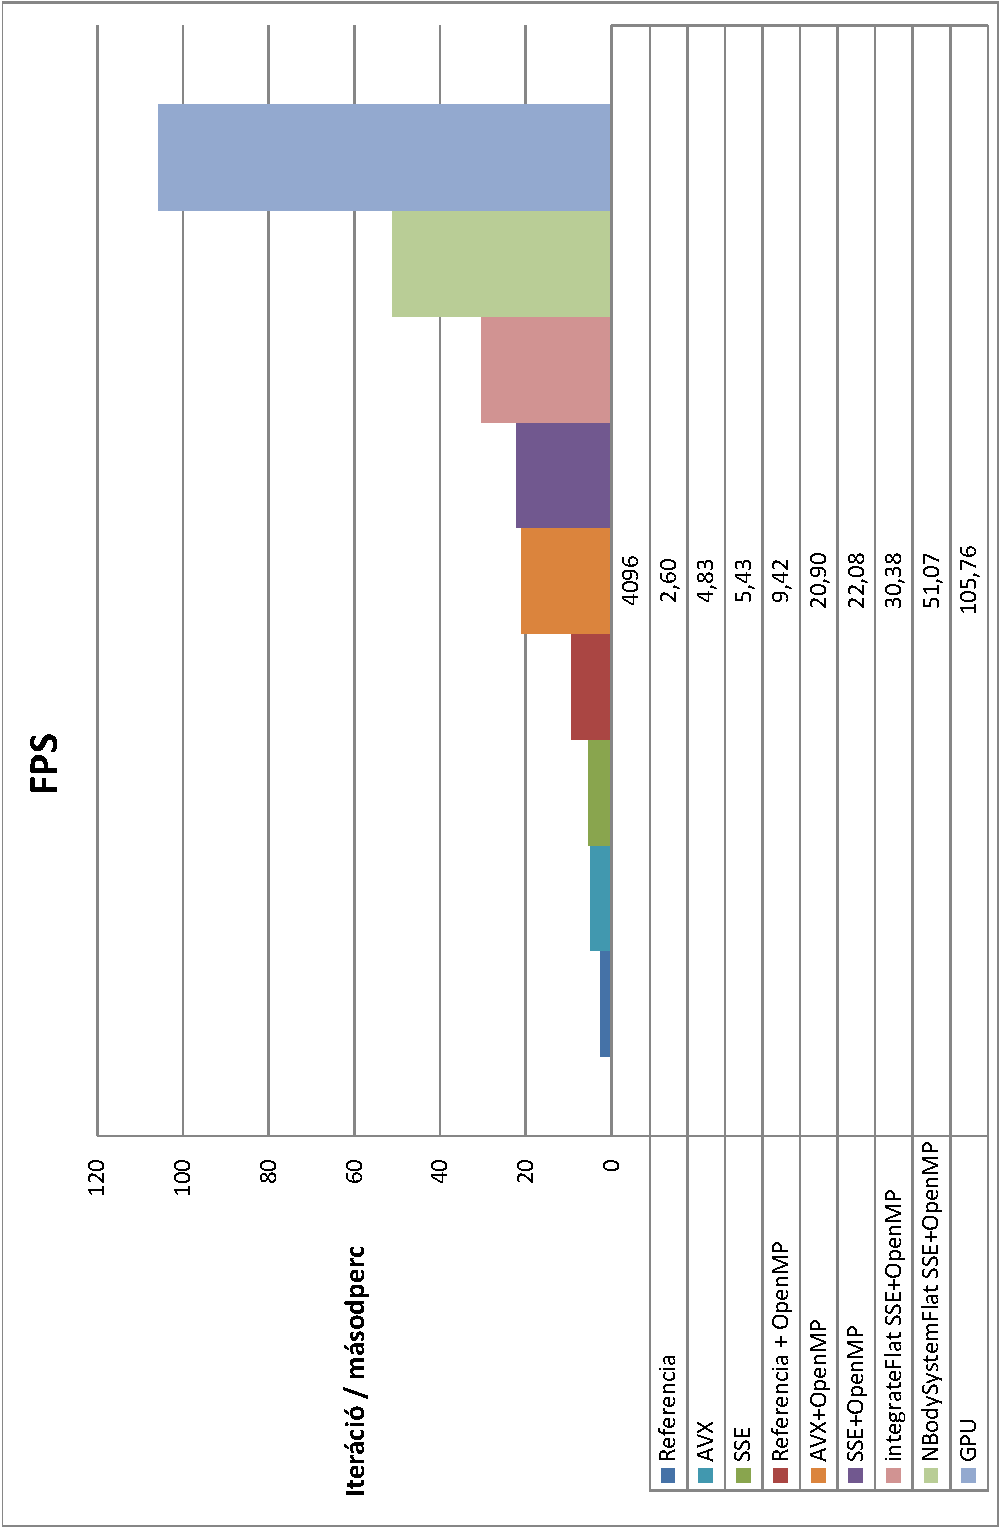
\includegraphics[width=150mm, keepaspectratio]{figures/Performance/FPS-cropped.pdf}
		\caption{Frame rate 4096 test eset�n}
		\label{fig:Perf_FPS}
	\end{figure}

	\begin{figure}[!ht]
		\centering
		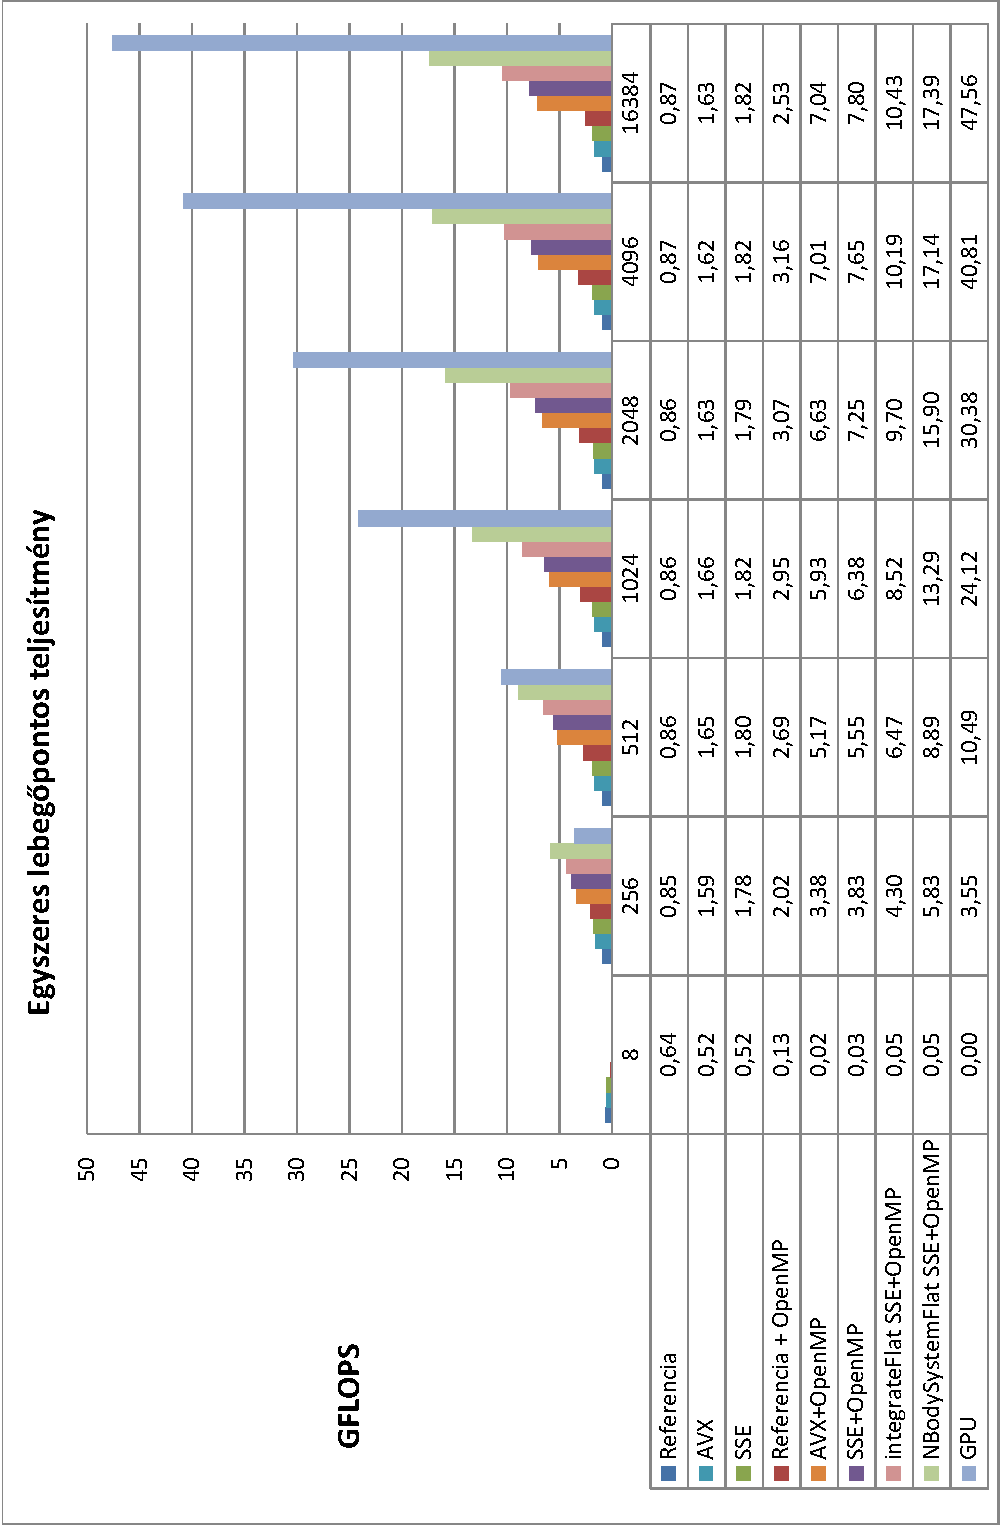
\includegraphics[width=150mm, keepaspectratio]{figures/Performance/GFLOPS-cropped.pdf}
		\caption{K�l�nb�z� konfigur�ci�k sz�m�t�si teljes�tm�nye}
		\label{fig:Perf_GFLOPS}
	\end{figure}

	\begin{figure}[!ht]
		\centering
		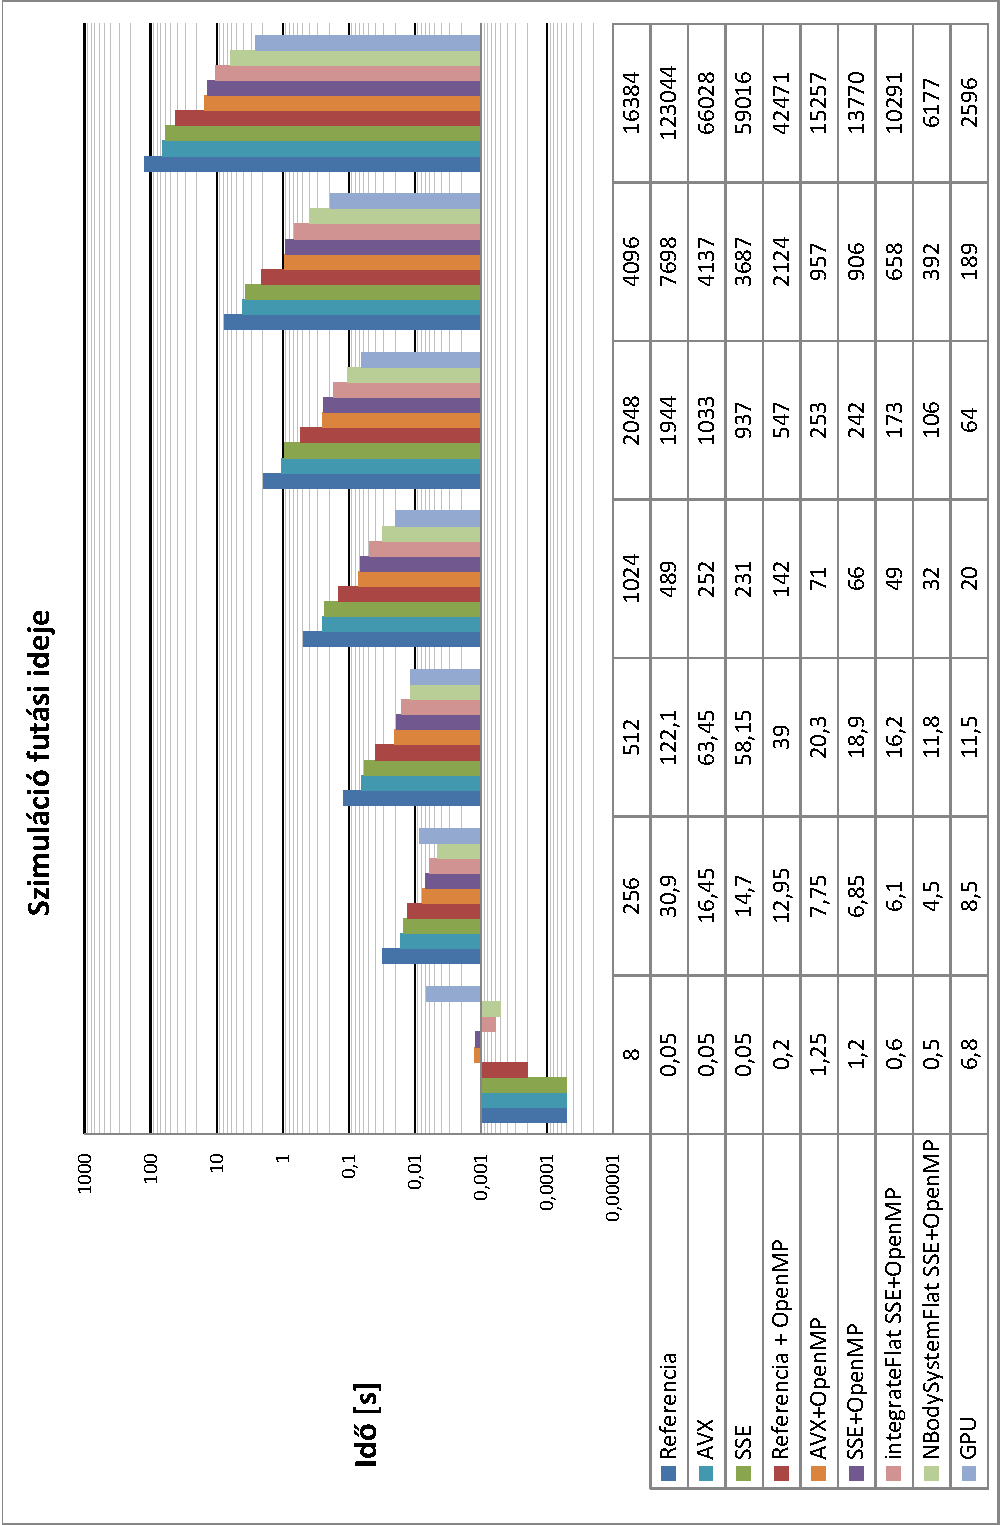
\includegraphics[width=150mm, keepaspectratio]{figures/Performance/FUTAS-cropped.pdf}
		\caption{K�l�nb�z� konfigur�ci�k fut�si ideje}
		\label{fig:Perf_FUTAS}
	\end{figure}

	


	

\label{page:last}
\end{document}

